\documentclass[
 reprint,
 superscriptaddress,
 amsmath,amssymb,
 aps,
]{revtex4-1}

\usepackage{graphicx}  
\usepackage{epstopdf}
\usepackage{dcolumn}
\usepackage{bm}	
\usepackage{amsmath}		
\usepackage{amsfonts}			
\usepackage{amssymb}			
\usepackage{latexsym}		
\usepackage{color}
\usepackage{ stmaryrd }
\usepackage[utf8]{inputenc}
\usepackage[english]{babel}
\usepackage{auto-pst-pdf} 


	\usepackage{epsf} 



\def\tc{\textcolor{red}}
\def\tg{\textcolor{green}}
\begin{document}

\title{ 
Forward scattering of a plane wave and of a spatially smoothed laser pulse  in the hydrodynamic and kinetic frameworks }
\author{C. Ruyer}\email{charles.ruyer@cea.fr}
\affiliation{CEA, DAM, DIF, F-91297 Arpajon, France}
\affiliation{Universit\'e Paris-Saclay, CEA, LMCE, 91680 Bruy\`eres-le-Ch\^atel, France}
\author{A. Debayle}
\affiliation{CEA, DAM, DIF, F-91297 Arpajon, France}
\affiliation{Universit\'e Paris-Saclay, CEA, LMCE, 91680 Bruy\`eres-le-Ch\^atel, France}
\author{P. Loiseau}
\author{P. E. Masson-Laborde}
\affiliation{CEA, DAM, DIF, F-91297 Arpajon, France}
\affiliation{Universit\'e Paris-Saclay, CEA, LMCE, 91680 Bruy\`eres-le-Ch\^atel, France}
\author{J. Fuchs}
\affiliation{LULI - CNRS, CEA, UPMC Univ Paris 06: Sorbonne Universit\'e, Ecole Polytechnique, Institut Polytechnique de Paris - F-91128 Palaiseau Cedex, France}
\author{M. Casanova}
\affiliation{CEA, DAM, DIF, F-91297 Arpajon, France}
\author{J. R. Marqu\`{e}s}
\affiliation{LULI - CNRS, CEA, UPMC Univ Paris 06: Sorbonne Universit\'e, Ecole Polytechnique, Institut Polytechnique de Paris - F-91128 Palaiseau Cedex, France}
\author{L. Romagnani}
\affiliation{LULI - CNRS, CEA, UPMC Univ Paris 06: Sorbonne Universit\'e, Ecole Polytechnique, Institut Polytechnique de Paris - F-91128 Palaiseau Cedex, France}
\author{P. Antici}
%\footnote{present address: INRS-EMT, 1650, boulevard Lionel-Boulet, J3X 1S2, Varennes (Québec), Canada}
\altaffiliation[present address: ]{INRS-EMT, 1650, boulevard Lionel-Boulet, J3X 1S2, Varennes (Qu\'ebec), Canada}
\affiliation{LULI - CNRS, CEA, UPMC Univ Paris 06: Sorbonne Universit\'e, Ecole Polytechnique, Institut Polytechnique de Paris - F-91128 Palaiseau Cedex, France}
\author{N. Bourgeois}
\altaffiliation[present address: ]{Central Laser Facility, STFC Rutherford Appleton Laboratory, Didcot OX11 0QX, United Kingdom}
\affiliation{LULI - CNRS, CEA, UPMC Univ Paris 06: Sorbonne Universit\'e, Ecole Polytechnique, Institut Polytechnique de Paris - F-91128 Palaiseau Cedex, France}
\author{M. Nakatsutsumi}
\altaffiliation[present address: ]{European XFEL, GmbH, Holzkoppel 4, 22869 Schenefeld, Germany}
%\footnote{present address: European XFEL, GmbH, Holzkoppel 4, 22869 Schenefeld, Germany}
\affiliation{Institute of Laser Engineering, Osaka University, 02-06 Yamada-Oka, Suita, Osaka, 565-0871, Japan}
\author{M. Safronova}
\affiliation{Institute of Applied Physics, RAS, 46 Ulyanov Street, 603950 Nizhny Novgorod, Russia}
\author{M. Starodubtsev}
\affiliation{Institute of Applied Physics, RAS, 46 Ulyanov Street, 603950 Nizhny Novgorod, Russia}
\author{T. Lin}
\affiliation{Fox Chase Cancer Center,
333 Cottman , Philadelphia, PA 19111-2497, USA} 

\begin{abstract}
We address the scattering of a high energy laser pulse on a large wavelength acoustic turbulence of relevance for LMJ or NIF-class  experiments. 
Both kinetic and hydrodynamic frameworks are adopted and combined with a linearized  description of the laser propagation. The resulting dispersion relations display important kinetic  contributions to the growth of the Forward Brillouin instability.  
Moreover, proof is made that the spatial incoherence  often used in high energy laser facilities are, for cold enough plasmas or in the multi-ion species case, not enough to reach full control of the laser filamentation.
Comparisons with experimental results and dedicated hydrodynamic 
simulations confirm our results. 
The   derived dispersion relations  present unique tools for assessing the propagation quality and energy deposition region of high energy laser pulses. They also underline the importance of accounting correctly for kinetic effects, even in the millimeters and nanoseconds scale of many  ICF or high-energy-density experiments. 
\end{abstract}

\maketitle 

\section{Introduction}
%\begin{itemize}
   % \item It requires the precise predictions of the  laser propagation along with parametric instabilities and their coupling with the smoothing technics, routinely used in high energy class facilities \cite[]{NatPhys_Glenzer,NatPhys_Labaune}.  
    %\item Forward instabilities such as filamentation \cite[]{phd_Michel,POP_michel_2003,Lushnikov_2006,PRL_Sarri_2011}, forward Brillouin  or plasma smoothing effects \cite[]{phd-Grech,POP_Grech_2006,PRL_Grech_2009} are vastly unexplored, and let's be honest, far more complicated than playing ping pong with positrons.
%\end{itemize}
High energy class laser facilities such as LMJ,  NIF or SG-III routinely bring matter under extreme conditions, not only of interest for inertial confinement fusion (ICF) \cite{Cavailler_2005,Lindl_2004,MRE_Zheng_2017}, but also for high energy astrophysics  and high energy density physics   \cite{Drake2006}. 
Whether the laser serves as a heat source or as a diagnostic, the accurate prediction of its propagation remains crucial for designing and  conceiving experiments. 
To this end, a large effort is made for understanding and mitigating the wave mixing processes able to scatter a significant part of the electromagnetic energy towards unwanted directions \cite[]{Shen_1965,Forslund_1973}. A better control of the laser propagation has been achieved experimentally by the use of Spectral Dispersion (SSD) and  Random Phase Plates (RPP) optical smoothing techniques\cite[]{Kato_1984,Skupski_1989,NatPhys_Glenzer,NatPhys_Labaune} and have been considered efficient to mitigate filamentation instability \cite[]{phd_Michel,POP_Michel_2003,Lushnikov_2006,PRL_Sarri_2011}, beam bending\cite[]{PRL_Hinkel_1996,
POP_Bezzerides_1998,PRL_Young_1998,POP_Ruyer_2020} and forward Brillouin.
To date, only stimulated backward Raman or Brillouin instabilities~\cite{POP_Liu_2009,hao_2013},  cross beam energy transfer \cite{hao_2016}, two plasmon decay \cite[]{Dubois_1995,Russell_2001} or collective scattering  \cite[]{PRL_Neuville_2016,PRL_Depierreux_2016}, are identified as critical issues in ICF, and remain active area of research. However, the small mitigation of cross beam energy transfer~\cite{PRL_Neuville_2016cbet} and backward Brillouin scattering by laser smoothing techniques may presage similar tendencies concerning the forward scattering. % and the laser beam filamentation. 
The latter can significantly alter the laser beam propagation by increasing the beam opening angle, thereby explaining the small laser beam transmission measured in some experiments~\cite{POP_Rousseaux_2015}.
 
To date, hydrodynamic codes remain the main tools to describe most of ICF experiments, due to their relatively affordable numerical cost. A first class of hydrodynamic codes, able to resolve the speckle scale structure, can describe different wave-mixing processes on a reduced plasma using regular meshes~\cite{Berger_1995,Still_2006,Loiseau_2006, Huller_2006}. However, the Landau damping rate which is the main parameter of wave-mixing processes in plasma, is reduced to an \emph{ad hoc} correction only valid in weakly-damped single-ion species plasma. Moreover, the non-local electron heat transport, thought to be important between each speckles during the heating phase~\cite[]{POP_Batishchev_2002,POP_Feugeas_2008}, is usually neglected. The second class of hydrodynamic codes, able to describe full scale ICF experiments on unstructured meshes, further neglects the speckle scale structure. The laser beam propagation is reduced to a ray-tracing scheme in which most of wave mixing processes are omitted. Recently, a ray-tracing algorithm has been proposed~\cite{POP_Debayle_2019} to self-consistently describe the cross beam energy transfer, the Raman and Brillouin backward scatterings. In principle, adding the convective growth of the filamentation and the forward Brillouin scattering are straightforward. However, this scheme neglects the speckle scale structure and assumes linear convective rates of wave-mixing processes based on a plane wave electromagnetic field. Alas, the resulting micron-scale speckle dynamics that interweaves with the wave mixing processes, brings further complexity to the theoretical and numerical analysis \cite[]{POP_Duluc_2019}. Building a self-consistent set of equations, adapted for Lagrangian hydrodynamic codes, that properly encompasses the filamentation instability, forward Brillouin  scattering and plasma smoothing effects \cite[]{phd-Grech,POP_Grech_2006,PRL_Grech_2009}, remains a challenging task.
%
%\emph{ad hoc} corrections or otherwise simply  omit, kinetic-based processes such as the particle trapping and subsequent wave-breaking \cite[]{POP_Benisti_2008,POP_Berger_2013}, two plasmon decay \cite[]{Dubois_1995,Russell_2001} or non-local thermal diffusion \cite[]{POP_Schurtz_2000,PRL_Froula_2007}, affecting the associated laser energy deposition. 
%
%\

This publication ambitions are to convey new tools 
able to address  the spatial growth of an electromagnetic scattered wave of wavevector and frequency close to the RPP pulse's and embedded in driven acoustic density fluctuations.
We first \tc{recall} both the kinetic and fluid \tc{derivation of the} forward scattering of a plane wave, limiting the study to the spatial  growth of  stimulated forward Brillouin scattering (FSBS) and the filamentation instabilities and pinpoint the importance of accounting for the kinetic plasma response for understanding quantitatively the scattering growth.
From  a simple model of RPP smoothed laser beam ensues our dispersion relations  able to predict the growth of the forward scatter relevant for high energy laser experiments \tc{and allowing to confront the predictability of fluid-based and kinetic simulations.} 
%\textcolor{red}{Dedicated "particle-in-cell" (PIC) simulations allows to validate our predictions and underline the importance of accounting for the laser smoothing in order to understand the forward Brillouin growth. Moreover, a
A comparison with dedicated hydrodynamic simulations and with an experiment conducted at the LULI facility validate our predictions.
%} 
The last section gather our perspective and concluding remarks. 

The SI unit system is used throughout this study while dropping the Boltzmann constant and vectors are noted in bold symbols. 

\section{Spatial growth of the  forward scattering of a plane wave}\label{sec:plane}
\subsection{Fluid and kinetic general dispersion relation}
The simplest way to obtain the growth of the forward scattering of a light wave propagating in a plasma consists  in combining the perturbed Maxwell equations with a linearized plasma response, either kinetic or fluid.
We aim at deriving and comparing in this section both frameworks.

Following Refs. \cite[]{Akhiezer_fluctuations,phd_Michel}, the perturbation of Maxwell equations around the laser field, $E_l$, \emph{i.e.} $E = E_l + \delta E$ and around the  electron density at rest $n_e = n_{e0}+\delta n_e$, gives in the Fourier space $(\omega_d,\mathbf{k}_d)$
\begin{equation}
    (\omega_d^2 - \omega_{pe}^2 -\mathbf{k}_d^2c^2)\delta E(\omega_d,\mathbf{k}_d) = \omega_0^2 \frac{\delta n_e }{n_c}\otimes E_l  \, ,\label{eq:max1}
\end{equation}
where $\omega_{pe}$, $\omega_{0}$,  $n_c$ and $c$ are the plasma and laser frequency, laser critical density and light speed in vacuum respectively. Use has also been made of $\otimes$ which designates  here a convolution product in the Fourier space.
Within the plane wave approximation,   $E_l=E_0 \cos(k_0 x - \omega_0t)$,
and we may write in the Fourier space,  
\begin{align}
   \mathrm{FT}_{\omega,\mathbf{k}}[ E_0 \cos(k_0 x - \omega_0t) ]= \nonumber\\ [ \delta(\omega-\omega_0, \mathbf{k}-\mathbf{k}_0) + \delta(\omega+\omega_0, \mathbf{k}+\mathbf{k}_0) ]E_0/2 \, , 
\end{align}
where $\mathrm{FT}[f(x,t)]$ designates the Fourier transform in space and time as $\frac{1}{(2\pi)^2}\int f(x,t) e^{-ikx+i\omega t}dxdt$. In this section,  $\mathbf{k}_0=k_0\hat{\mathbf{x}}$ is the $x$-aligned pump wavevector ($\hat{\mathbf{x}}$ is the unity vector along the $x$ axis), thus giving 
\begin{align}
    (\omega_d^2 - \omega_{pe}^2 -\mathbf{k}_d^2c^2)\delta E(\omega_d,\mathbf{k}_d) = \frac{\omega_0^2}{2} E_0\times \nonumber\\ \left[\frac{\delta n_e }{n_c}(\omega_d-\omega_0, \mathbf{k}_d-\mathbf{k}_0) +\frac{\delta n_e }{n_c}(\omega_d+\omega_0, \mathbf{k}_d+\mathbf{k}_0) \right] \, .\label{eq:max2}
\end{align}

The final dispersion relation  can be obtained by combining this equation with a linearized plasma response, which, in the fluid framework~\cite{POP_Ruyer_2020} and for a plasma at rest, %($v_d=0$) 
reads 
\begin{align}
   \frac{\delta n_e }{n_{e0}}(\omega_s,\mathbf{k}_s) = \frac{-\kappa\mathbf{k}^2c_s^2}{ \mathbf{k}_s^2c_s^2-\omega_s^2 -2i\omega_s \nu} \frac{A_k\epsilon_0 E_0}{n_c T_e}\times \nonumber\\ \left[\delta E(\omega_s-\omega_0, \mathbf{k}_s-\mathbf{k}_0) +\delta E(\omega_s+\omega_0, \mathbf{k}_s+\mathbf{k}_0) \right] \, .\label{eq:fluid}
\end{align}
Here, $\kappa = Z_iT_e/m_ic_s^2$,  $c_s\simeq [(Z_iT_e+3 T_i)/m_i]^{1/2}$, $\nu=\vert\mathbf{k}_s\vert \gamma_0 c_s$ and $A_k$, are respectively  the sound speed, the Landau damping frequency and a non-local thermal correction to the ponderomotive force \tc{\cite[]{POP_Kaiser_1993,Bychenkov_2000}}, 
\begin{align}
     A_k(u)   &= \frac{1}{2} +Z_i\left( \frac{0.074}{u^2}+ \frac{0.88}{u^{4/7}} + \frac{2.54}{1+5.5u^2} \right) \, ,\nonumber \\ 
     u &=\vert \mathbf{k}_s \vert\lambda_\mathrm{mfp} \sqrt{Z_i}\label{eq:nl}\, .
\end{align}
We also made use of $T_{e/i}$, $m_{e/i}$ $Z_i$ and $\lambda_\mathrm{mfp}$, the electron/ion temperature and mass, ion charge number and electron mean-free-path, respectively. For a multi-ion species plasma, the smallest mean-free-path among the ion species is used to compute $A_k$ \tc{ and the value of $c_s$ is computed on the mean-ion parameters ($Z_i$ , $A_i$ and $T_i$). Hence, especially in the mutli-ion species case, $c_s$ does not necessarily coincide with the solution of the acoustic dispersion relations that may present one fast and one slow mode in the multi ion species case  \cite[]{POF_Fried_71,POP_Williams_95}.}  
The correction of  Ref. \cite[]{Bychenkov_2000} requires to account for the collisional acoustic damping rate which is negligible for the plasma parameters addressed here ($T_e\gtrsim 1\,\rm keV$, $n_e\le 10^{21}\,\rm cm^{-3}$ and $I_0\le 10^{15}\rm W/cm^{2}$) or irrelevant (as for the filamentation instability, Secs.  \ref{sec:filam} and \ref{sec:xp}).
Note that, for the parameters explored in this study, the non-local correction remains non negligible and therefore essential to obtain realistic predictions \cite[]{PRL_Epperlein_1990,POP_Berger_2005}.  

In the following, 
the normalized acoustic wave Landau damping rate, $\gamma_0$, 
\begin{align}
\gamma_0 &= \sqrt{\frac{2T_i }{m_ic_s^2 }} 
\Im\left[
\frac{  \mathcal{Z}'\left(x_i\right) 
+\frac{T_i}{Z_iT_e}  \mathcal{Z}'\left(x_e\right)   }{  \mathcal{Z}''\left(x_i\right) +\left(\frac{T_i}{Z_iT_e}\right)^{3/2}\sqrt{\frac{Z_im_e}{m_i}}  \mathcal{Z}''\left(x_e\right)    }
\right]\, , \nonumber \\
x_{e/i}&=\sqrt{\frac{m_{e/i}c_s^2}{2T_{e/i}}}\, ,\label{eq:g0}
\end{align}
will be used under the assumptions  $\nu/\vert \mathbf{k}_\perp \vert c_s= \gamma_0 \ll 1$, $\vert \mathbf{k}_\perp \vert\lambda_{Di}\ll 1$.
$\lambda_{De/i}$ is the electron/ion Debye length and $ \mathcal{Z}$ is the plasma dispersion function \cite{Fried_Gell-Mann_1960}.

Likewise, the kinetic counterpart of Eq. \eqref{eq:fluid} has been derived in Ref. \cite[]{POF_Drake_1973} and prevails in the case of a multiple ion Maxwellian plasma. It writes
\begin{align}
 \frac{ \delta n (\omega_s, \mathbf{k}_s ) }{n_{e0}}  =   \frac{ \epsilon_0  E_0 }{ 2n_c T_e } 
 \frac{\mathcal{Z}'( \zeta_e) }{2}
 \frac{\sum_i\mathcal{Z}'( \zeta_i)\frac{  Z_iT_e}{ T_i }\frac{  Z_in_i}{ n_e }   }{  \mathcal{Z}'( \zeta_e)+ \sum_i\mathcal{Z}'( \zeta_i)\frac{  Z_iT_e}{ T_i }\frac{ Z_i n_i}{ n_e }  }
 % \frac{\mathcal{Z}'( \xi_i)   }{  \mathcal{Z}'( \xi_i) +\mathcal{Z}'( \xi_e)\frac{ T_i }{  ZT_e} }
\nonumber\\  \times \left[\delta E(\omega_s-\omega_0, \mathbf{k}_s-\mathbf{k}_0) +\delta E(\omega_s+\omega_0, \mathbf{k}_s+\mathbf{k}_0) \right] %\nonumber \\  &\times 
   \, ,\label{eq:drake}\\
   \zeta_{e/i} = \frac{   \omega }{   \vert\mathbf{k}_s\vert }  \sqrt{ \frac{ m_{e/i } }{ 2T_{e/i }}  }  \label{eq:xi} \, , 
 \end{align}
 where we also assumed $\vert k_s \lambda_{Di} \vert \ll 1$. 

To unify the fluid and kinetic descriptions, we introduce the parameters
\begin{align}
   \alpha_k  = \frac{-\mathcal{Z}'( \zeta_e) }{2}
 \frac{\sum_i\mathcal{Z}'( \zeta_i)\frac{  Z_iT_e}{ T_i }\frac{  Z_in_i}{ n_e }   }{  \mathcal{Z}'( \zeta_e)+ \sum_i\mathcal{Z}'( \zeta_i)\frac{  Z_iT_e}{ T_i }\frac{ Z_i n_i}{ n_e }  }\, ,\label{eq:alphak} \\
   \alpha_f = \frac{\kappa c_s^2}{ c_s^2-v_\phi^2 -2iv_\phi c_s \gamma_0}\, .\label{eq:alphaf}
\end{align}
where $v_\phi = \omega_s/\vert \mathbf{k}_s\vert $ is the phase velocity.
Both Eqs. \eqref{eq:fluid} and  \eqref{eq:drake} recast as:
\begin{align}
   \frac{\delta n_e }{n_{e0}}(\omega_s,\mathbf{k}_s) = -\alpha_{k/f}(v_\phi) \frac{A_k\epsilon_0 E_0}{n_c T_e}\times \nonumber\\ \left[\delta E(\omega_s-\omega_0, \mathbf{k}_s-\mathbf{k}_0) +\delta E(\omega_s+\omega_0, \mathbf{k}_s+\mathbf{k}_0) \right] \, ,\label{eq:fd}
\end{align}
Note that we have  applied the non-local correction [Eq. \eqref{eq:nl}] in the kinetic framework, as there is, to the best of our knowledge,  no better simple alternative. Originally derived in the fluid framework, its proper kinetic counterpart would require to \tc{replace the ion fluid response of Ref. \cite[]{POP_Berger_2005} by a kinetic one in order to model Coulomb collisions effects in multi-ion species plasmas \cite[]{POP_Berger_2005b} or to start from Refs. \cite[]{POP_Epperlein_94,POP_Bychenkov_1998}, such analysis } is out of the scope of the present study. As the $A_k$-factor is relevant in the fluid framework, choice has been made to include it in the kinetic formalism for comparison purposes. Yet, its use is questionable regarding the forward Brillouin predictions.

From the combination of  Eqs. \eqref{eq:max2} with \eqref{eq:fd}, 
for $D_\pm= (\omega_s\pm \omega_0)^2 - \omega_{pe}^2 -( \mathbf{k}_s\pm \mathbf{k}_0) ^2c^2 $, ensues
\begin{equation}\label{eq:dispe}
    D_+D_- = -\omega_{0}^2\alpha_{k/f}A_k\frac{\delta n_0}{n_c} (D_++D_-) \, ,
\end{equation}
with $\delta n_0/n_c = (n_{e0}/n_c) \epsilon_0E_0^2/(2n_c T_e)$.
Note that we neglected the terms in $\delta n_e(\omega_s \pm 2\omega_0)$.
In the kinetic framework, the above equation corresponds to Eq. (36) of Ref. \cite[]{POF_Cohen_79} in the limit $\vert k_s \lambda_{Di} \vert \ll 1$. In the fluid framework, similar equations were derived in Refs. \cite[]{Kruer,phd_Michel,phd-Grech}.

\subsection{Spatial growth of the filamentation and of the forward Brillouin instability}

\begin{figure}
\begin{tabular}{cc}
(a) Kinetic, $\Gamma/k_0$ &
(b)  Kinetic, $\Re(k_{sx}/k_0)$ \\
%\includegraphics[width=0.24\textwidth]{1a.png}&
%\includegraphics[width=0.24\textwidth]{1b.png}\\
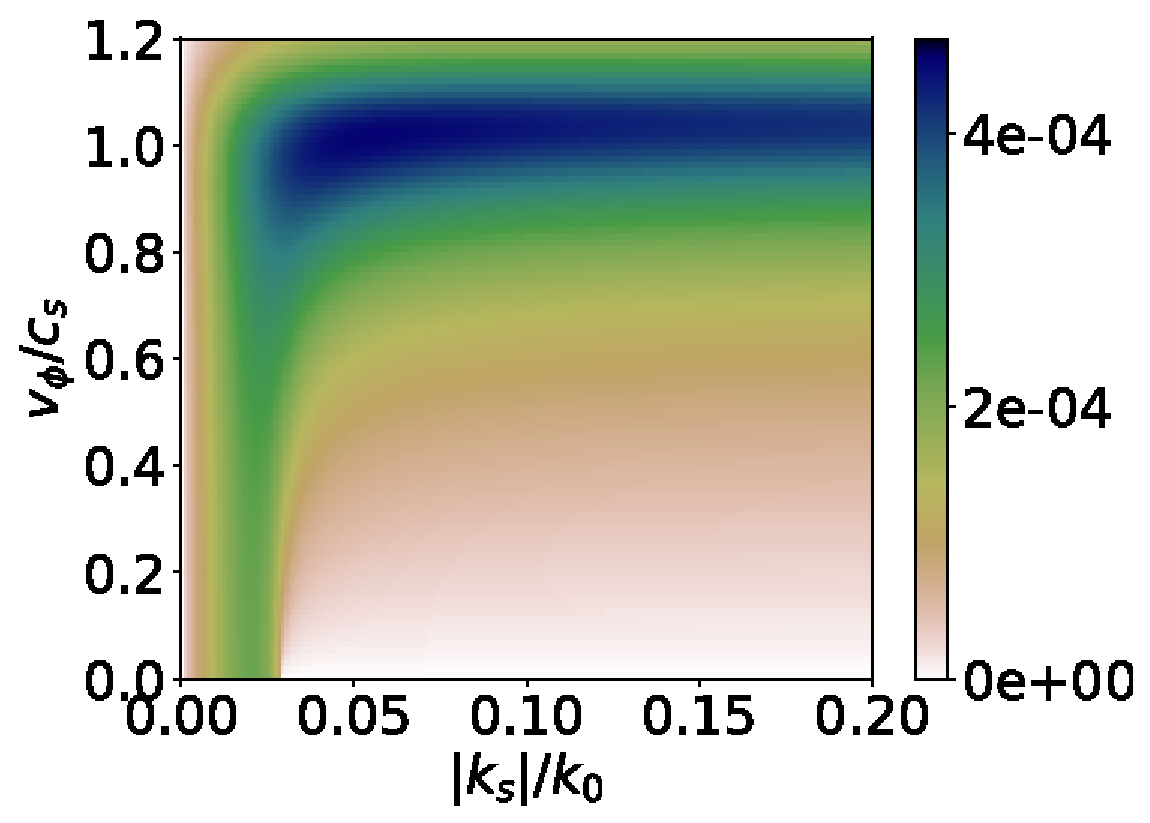
\includegraphics[width=0.24\textwidth]{Fig1a.eps}&
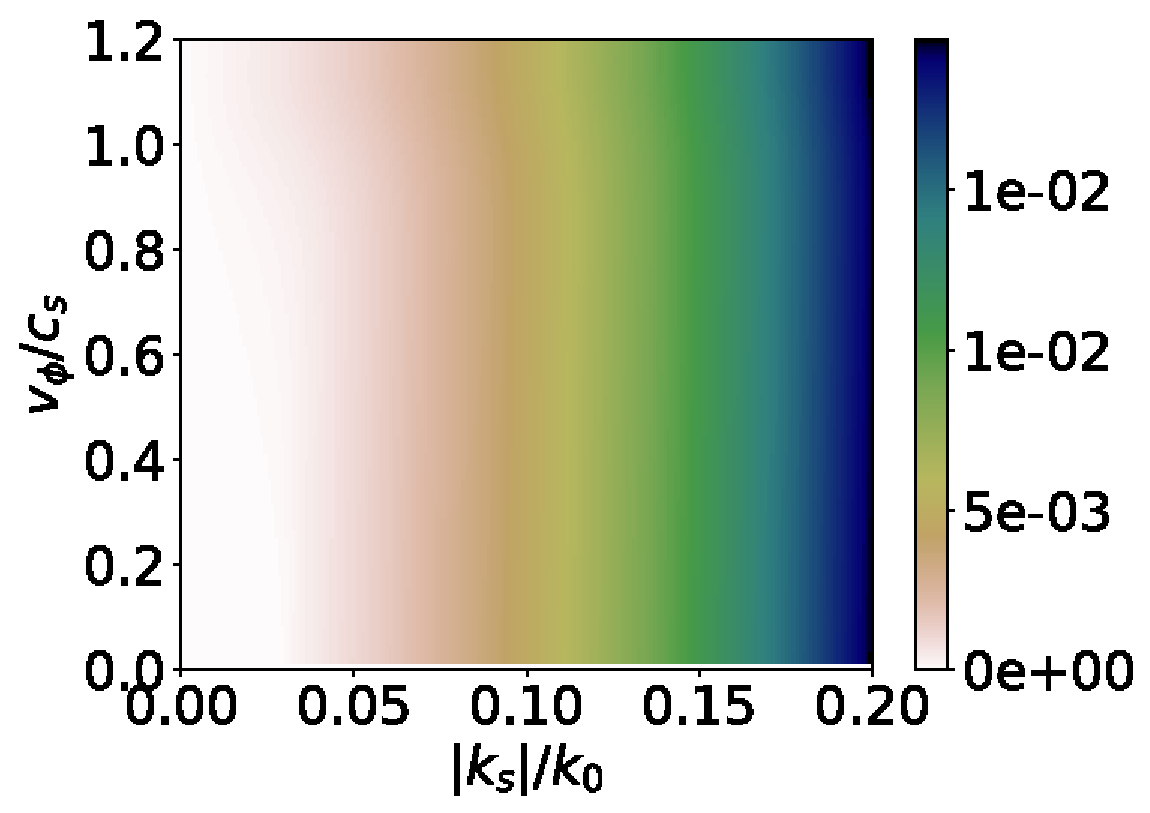
\includegraphics[width=0.24\textwidth]{Fig1b.eps}\\
(c) Fluid, $\Gamma/k_0$  &
(d) Fluid, $\Re(k_{sx}/k_0)$  \\
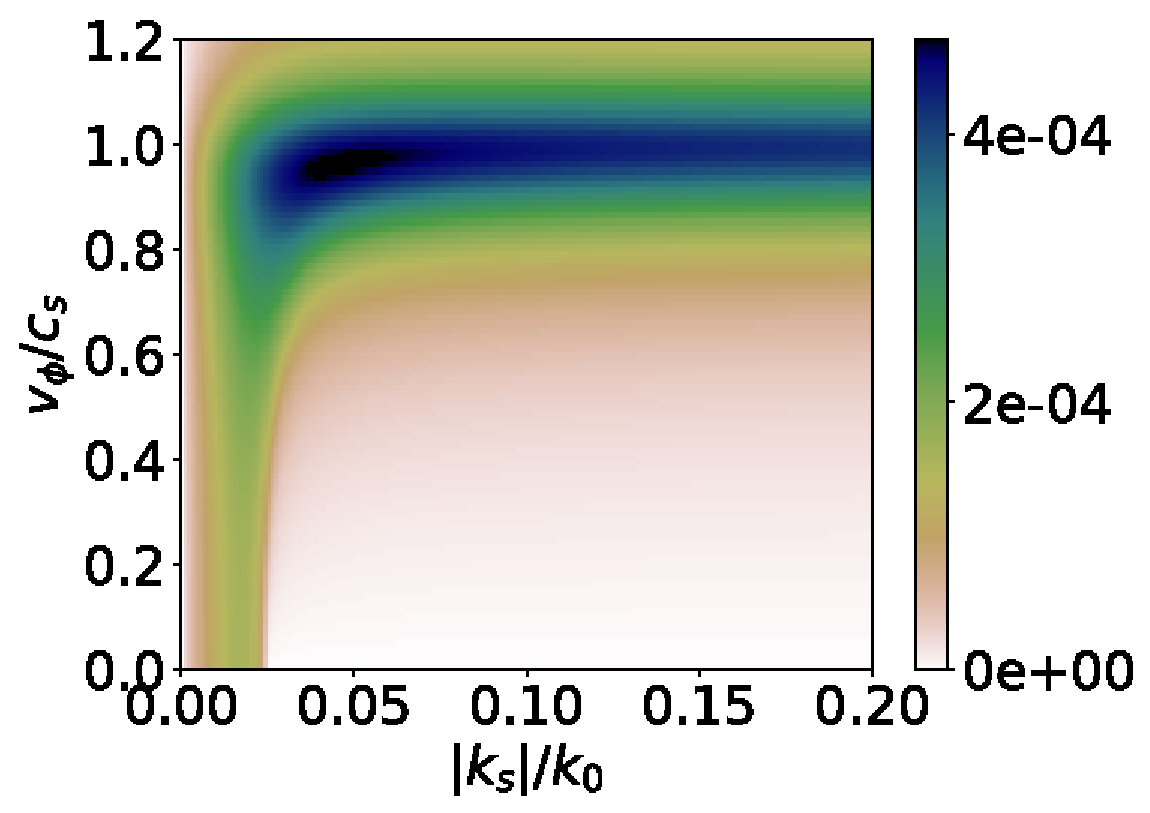
\includegraphics[width=0.24\textwidth]{Fig1c.eps}&
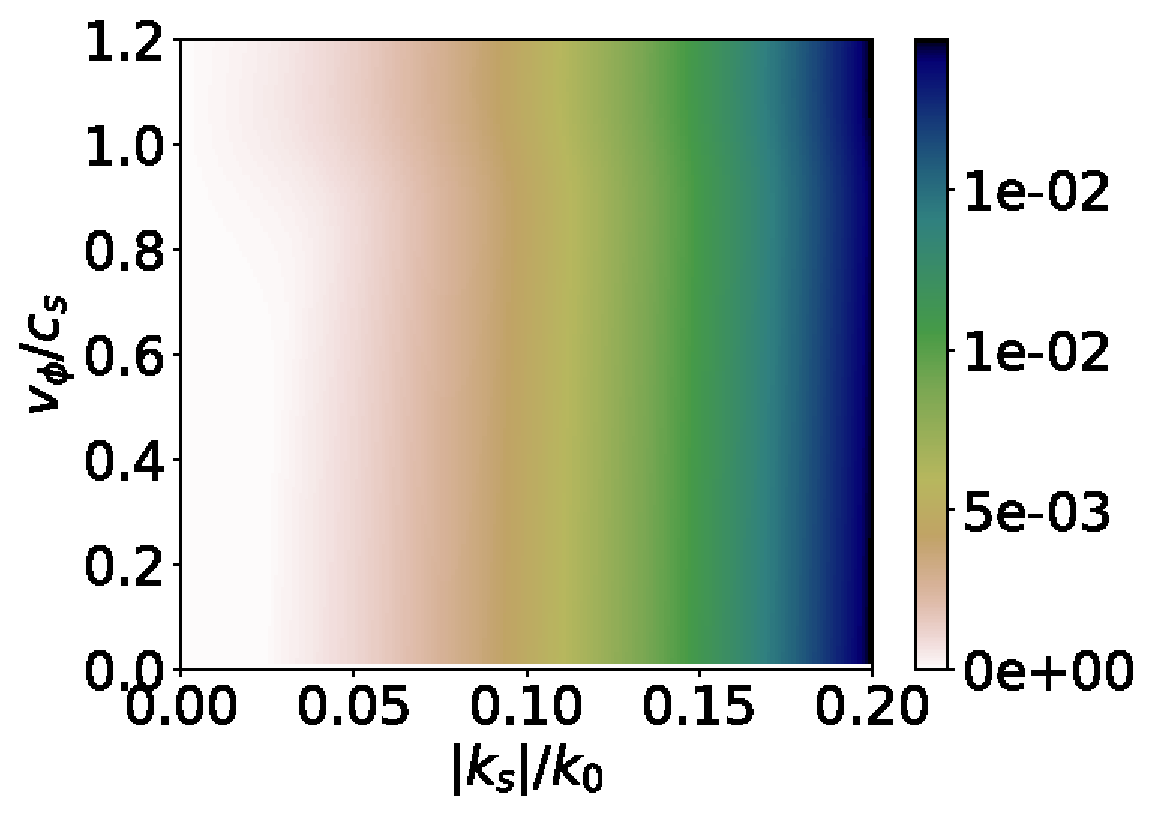
\includegraphics[width=0.24\textwidth]{Fig1d.eps}
\end{tabular}
\caption{ \label{fig:dispe}  
Kinetic (a,b) and fluid (c,d) resolution of Eq. \eqref{eq:dispe2poly} for  $I_0 = 6\cdot 10^{14}\, \rm W.cm^{-2}$, $2\pi/k_0=0.35 \,\rm\mu m$, $T_e =1\,\rm  keV$, $ T_i=300\,  \rm eV$ in a H$^+$ and $n_{e0}=0.1n_c$.
 }
\end{figure}
Hence,  making use of $\omega_0^2=\omega_{pe}^2 +k_0^2c^2$, we may simplify $D_\pm$ to leading order in $\omega_s\ll\omega_0$, as done in Ref. \cite[]{POP_Kaiser_1993}, giving  
\begin{equation}\label{eq:dpm}
D_\pm = -\mathbf{k}_s^2c^2\pm 2(\omega_s\omega_0 - \mathbf{k}_s\cdot\mathbf{k}_0 c^2) \, .
\end{equation} 
Equation \eqref{eq:dispe} thus becomes 
\begin{equation}\label{eq:dispe2} 
(\omega_s\omega_0 - \mathbf{k}_s\cdot\mathbf{k}_0 c^2)^2
=\frac{\mathbf{k}_s^2c^2}{4}\left( \mathbf{k}_s^2c^2 - 2\omega_{0}^2\alpha_{k/f}(v_\phi)A_k\frac{\delta n_0}{n_c} \right) 
\, .
\end{equation}

The spatial growth of the filamentation instability may be recovered when $\omega_s$=0 and assuming $\mathbf{k}_s = -i\Gamma_F\hat{\mathbf{x}} + k_s \hat{\mathbf{y}}$,
\begin{equation}\label{eq:gf} 
\Gamma_F^2
=\frac{\mathbf{k}_s^2}{4k_0^2c^2}\left( 2\omega_{0}^2\alpha_{k/f}(0)A_k\frac{\delta n_0}{n_c}- \mathbf{k}_s^2c^2 \right) 
\, .
\end{equation}
Note that for a single ion species,  $\alpha_f(0)=1$ and $\alpha_k(0)= Z_iT_e/T_i/(1+Z_iT_e/T_i)$ so that the kinetic and fluid frameworks coincide in the limit $Z_iT_e/T_i\gg 1$.

As for the \tc{backward} Brillouin scattering  corresponding to the limit $1/D_-\gg1/D_+$, non vanishing acoustic wave frequencies are obtained with  phase speeds of the order of the sound speed. We propose to address the spatial growth of both the filamentation and forward Brillouin instabilities  by solving Eq. \eqref{eq:dispe2} for  $\mathbf{k}_s = k_{sx} \hat{\mathbf{x}} +k_{sy} \hat{\mathbf{y}}$, and assuming 
$ k_{sy}$ and $k_{sx}$ purely real and complex  respectively. Equation \eqref{eq:dispe2} then becomes 
\begin{equation}\label{eq:dispe3} 
\left(\frac{v_\phi}{\eta c} - 
\frac{ k_{sx}}{\vert \mathbf{k}_s\vert }\right)^2
=\frac{1}{4} \left( \frac{\mathbf{k}_s^2}{k_0^2} - 2\alpha_{k/f}(v_\phi)A_k\frac{\delta n_0}{\eta^2n_c} \right) 
\, ,
\end{equation}
where $\eta=\sqrt{1-n_{e0}/n_c}$ is the refraction index.
Hence, $u =  k_{sx}/\vert \mathbf{k}_s\vert $ is solution of the following second order polynomial equation, 
\begin{equation}\label{eq:dispe2poly} 
u^2 -2\frac{v_\phi}{\eta c}u +\frac{v_\phi^2}{\eta^2 c^2}-\frac{1}{4}\left( \frac{\mathbf{k}_s^2}{k_0^2} - 2\alpha_{k/f}(v_\phi)A_k\frac{\delta n_0}{\eta^2n_c} \right) =0 
\, .
\end{equation}
%To leading order in  $\Im(k_{sx})/\vert \mathbf{k}_s\vert $ (where $\Im$ and $\Re$ are the imaginary and real part of a complex), $\vert \mathbf{k}_s\vert$ and $v_\phi$ may be considered to be purely real.

\begin{figure}
\begin{tabular}{cc}
(a) Kinetic, $\Gamma/k_0$ &
(b)  Kinetic, $\Re(k_{sx}/k_0)$ \\
%\includegraphics[width=0.24\textwidth]{2a.png}&
%\includegraphics[width=0.24\textwidth]{2b.png}\\
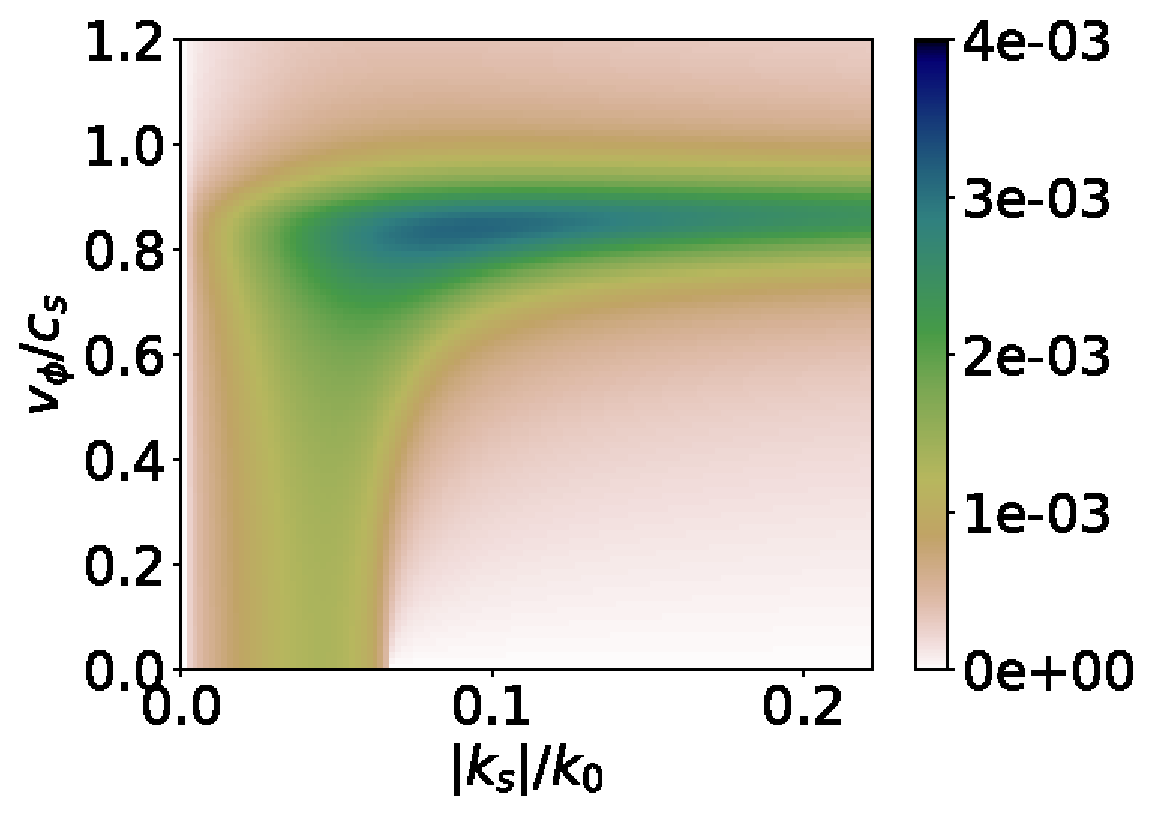
\includegraphics[width=0.24\textwidth]{Fig2a.eps}&
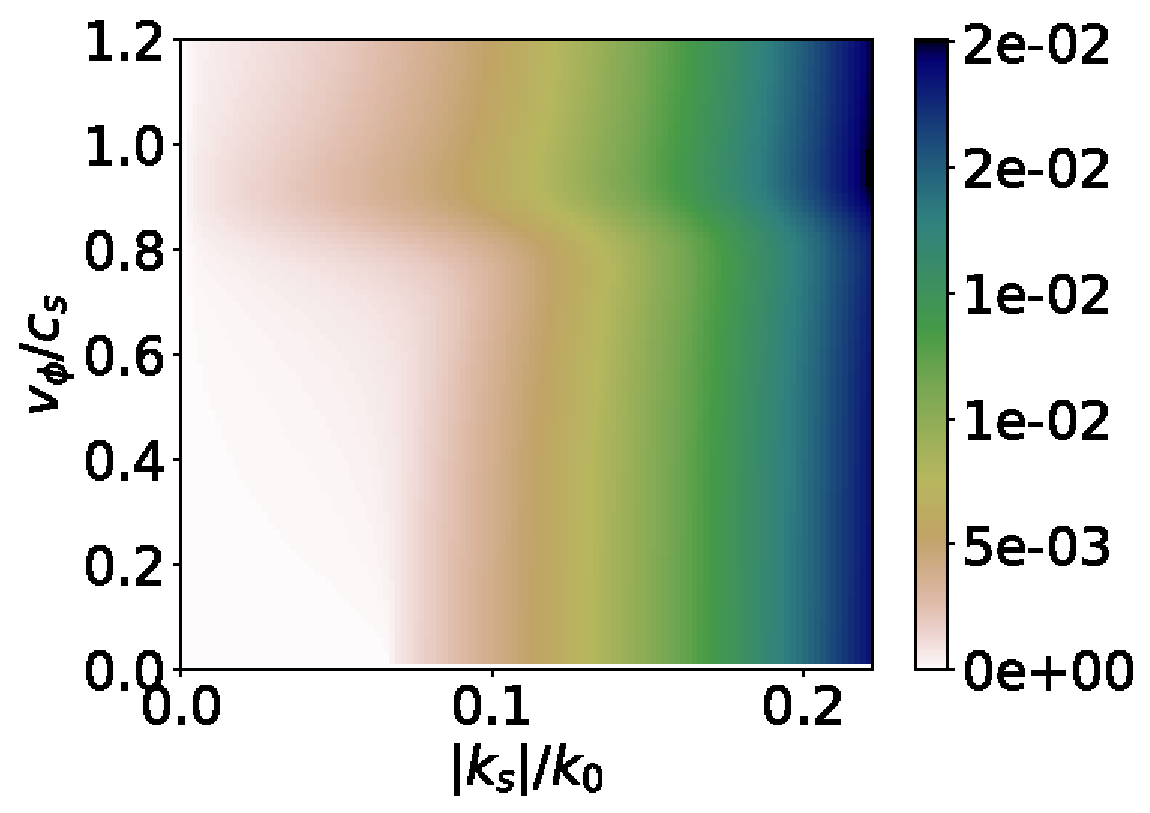
\includegraphics[width=0.24\textwidth]{Fig2b.eps}\\
(c) Fluid, $\Gamma/k_0$  &
(d) Fluid, $\Re(k_{sx}/k_0)$  \\
%\includegraphics[width=0.24\textwidth]{2c.png}&
%\includegraphics[width=0.24\textwidth]{2d.png}
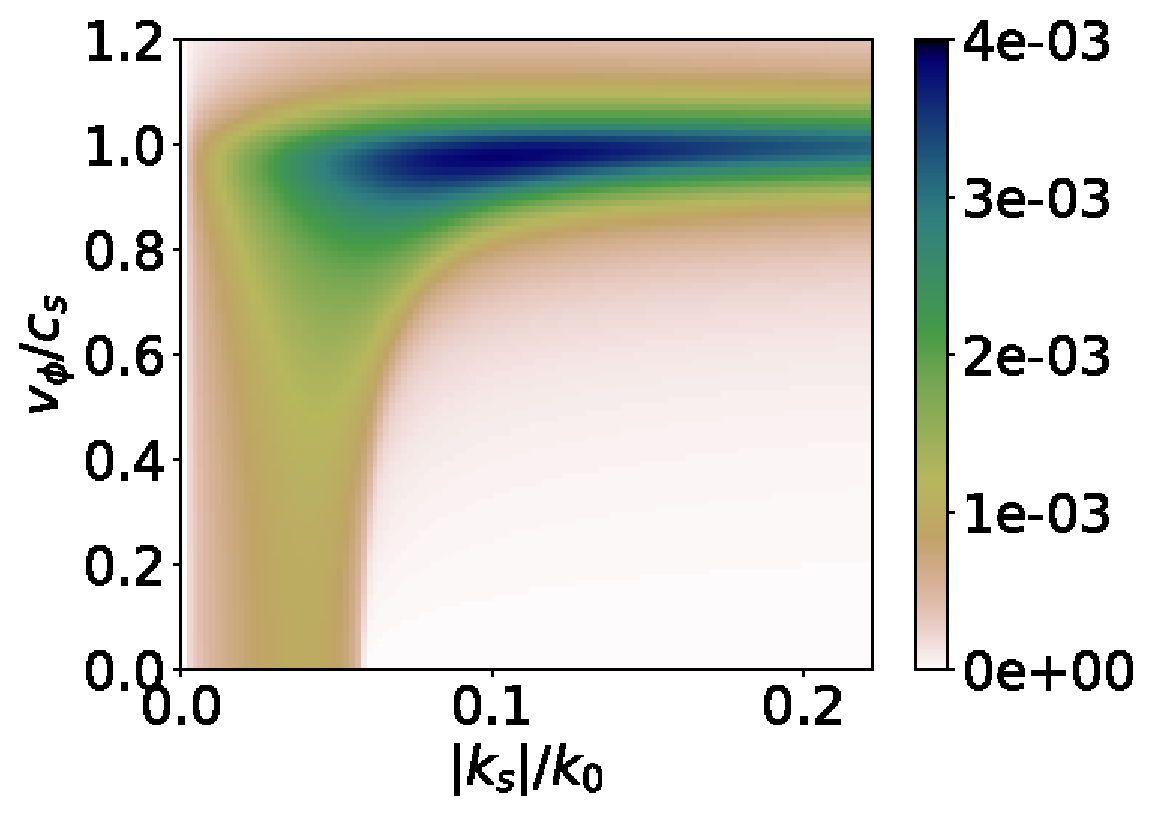
\includegraphics[width=0.24\textwidth]{Fig2c.eps}&
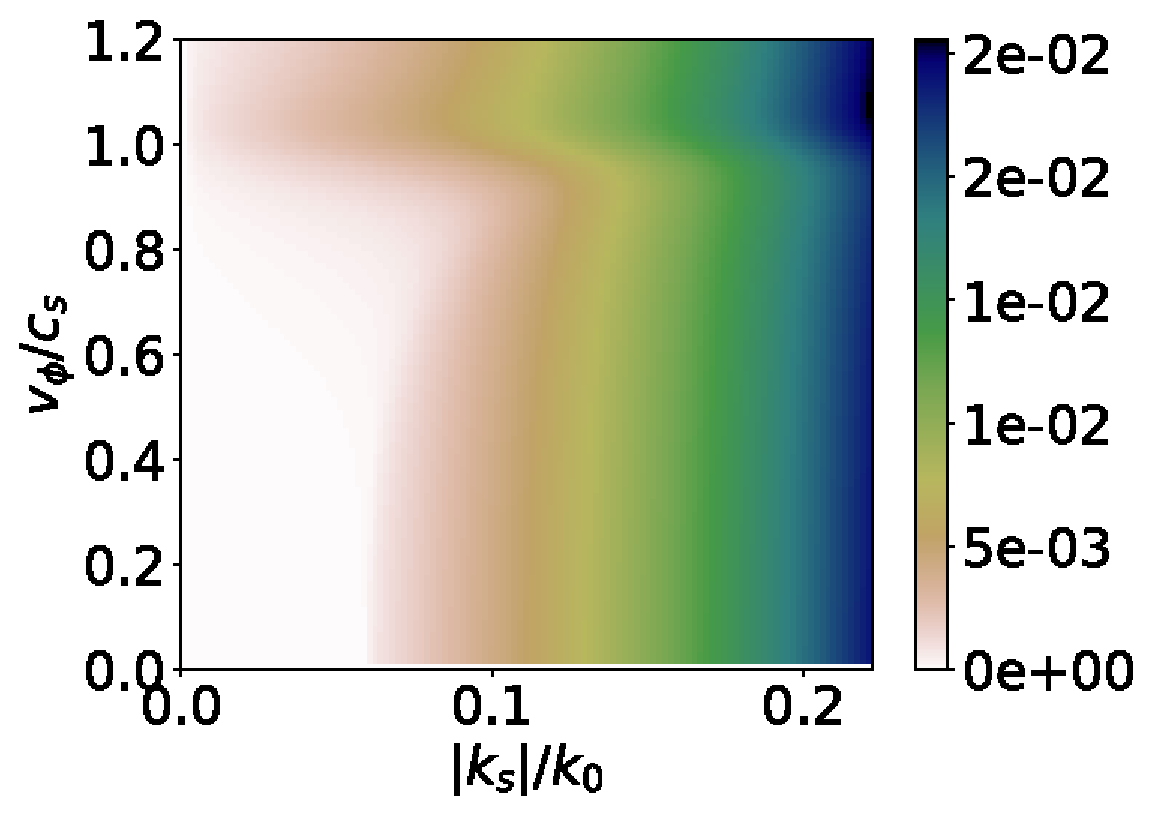
\includegraphics[width=0.24\textwidth]{Fig2d.eps}
\end{tabular}
\caption{ \label{fig:dispeCH}  
Kinetic (a,b) and fluid (c,d) resolution of Eq. \eqref{eq:dispe2poly} for  $I_0 = 6\cdot 10^{14}\, \rm W.cm^{-2}$, $2\pi/k_0=0.35 \,\rm\mu m$, for a CH plasma with $n_c=n_H$, $T_e =700\,\rm  eV$, $T_C=T_H =500\,  \rm eV$ and $n_{e0}=0.1n_c$. The value of the non-local correction [Eq. \eqref{eq:nl}], is obtained with the carbon parameters, corresponding to the smallest electron-ion mean-free-path. Use is made of the mean charge number, mean mass number   for calculating the sound speed and normalized Landau damping rate $c_s$ and $\gamma_0$.
 }
\end{figure}
Figures \ref{fig:dispe}(a-d) display  $\Re(k_{sx})$ and the spatial growth rate,  $\Gamma=-\Im(k_{sx})$, combining   the  unstable parts of the two  solutions of Eq. \eqref{eq:dispe2poly} as a function of the phase speed and of the wavevector amplitude, in both the kinetic (a,b) and fluid frameworks (c,d).
The filamentation limit is recovered at $v_\phi=0$ and care has been taken to verify that both frameworks co\"incide, when $T_i\ll Z_iT_e$. Moreover, in both calculations, $\Re[k_{sx}(v_\phi=0)]$ is vanishing as expected from the filamentation instability. As $v_\phi$ increases, the forward Brillouin instability prevails and reaches its maximum, for the kinetic  mono-ion species case of Fig. \ref{fig:dispe}(a), around $(\vert k_s\vert/k_0, v_\phi/c_s) \simeq(0.05,1)$. 
%Interestingly, only in the kinetic framework  the forward Brillouin spatial maximum  growth dominates the filamentation one, for the plasma parameters addressed here. 
\tc{
In the fluid framework, a similar behavior is obtained, although with a slightly larger forward Brillouin spatial  growth maximum. }

The kinetic calculations allow to consider multiple ion plasmas such as CH as illustrated in Fig. \ref{fig:dispeCH}. In the fluid framework, we are usually constrained to use the averaged-ion approximation, which gives qualitatively similar results than for Fig. \ref{fig:dispe}(c) as a broad spectrum is evidenced with  dominance of the Brillouin versus the filamentation growth. 
%This contrasts with the kinetic calculations of Fig. \ref{fig:dispeCH}(a) where the FSBS is more unstable than the filamentation instability. 
Moreover the growth is peaked around $0.8c_s$ (here $c_s$ is calculated on the averaged ion parameters) which is the phase speed of the least-damped acoustic eigenmode, solution of the free-field electrostatic Maxwellian dispersion relation \cite[]{POF_Fried_71,POP_Williams_95}.
Notably, the forward Brillouin growth rate is \tc{ $\sim 25\%$ smaller} in the kinetic formalism compared to the fluid description. This substantial difference, visible in both the hydrogen  and  CH plasma, vanishes in the case of the filamentation instability where both frameworks predict similar growth rates.
This driven ion acoustic wave ($\vert v_\phi\vert >0$) is able to  scatter the pump wave and modify its spatial spectrum. As evidenced in Figs. \ref{fig:dispe}(a,c) and \ref{fig:dispeCH}(a,c), we expect a broadening of the plane wave spatial spectrum  resulting in an effective  f-cone   angle  of $k_s/k_0\sim 0.03-0.05$, corresponding to $\sim 2-3^o$.  

Spatial smoothing techniques are commonly known to restrain the role of some deleterious instabilities, such as the laser filamentation, during the propagation of energetic laser pulses  \cite[]{Kato_1984,NatPhys_Glenzer,POP_Berger_98b}. Indeed, as shown in this section, the most unstable wavelength, regarding the filamentation or the forward Brillouin instabilities, is of the order of ten   microns (for $\sim$ keV and 10\% critical density plasmas), thus larger than the typical  speckle size   of a few microns   usually used in energetic laser facilities.  
Hence, the plane wave approximation used in obtaining Eq. \eqref{eq:max2} no longer holds and one might expect a more stable pump propagation.
Yet, although extensively studied in the fluid framework by mean of numerical or theoretical tools \cite[]{POP_Schmitt_Afeyan_98,POP_Hinkel_1998,PRL_Myatt_2001,POP_Maximov_2001,Lushnikov_2006,phd-Grech,POP_Grech_2006,PRL_Grech_2009}, to the best of our knowledge, no analytical attempts were done to estimate the spatial growth of the forward Brillouin scattering of a RPP pulse in the kinetic framework. 
We propose in next section to adapt the above analytical plane wave dispersion relations  to tackle this issue.

 \begin{widetext}
\section{Forward scattering of a spatially smoothed laser pulse}
\subsection{Kinetic and fluid dispersion relations}\label{sec:diperpp}
The RPP beam model adopted here has been introduced in  Refs. \cite[]{POF_Schmitt_88,POF_Rose_93} and presents an electric field, $E_{\rm RPP}$, of the form
 \begin{align}
E_{\rm RPP}(t,\mathbf{r})  = \frac{E_0}{N} \sum_{n,\vert k_{\perp}\vert<k_m }^N  \cos(k_0x - \omega_0t +\mathbf{k}_\perp(n) \cdot \mathbf{r}_\perp +\Phi_{\mathbf{k}_\perp})\, , \label{eq:erpp}
 \end{align}
 where  $N$ is the number of diffracting elements and the phases $\Phi_{\mathbf{k}_\perp}$ are  independent random variables taking the values $0$ or $\pi$ with equal probability.
 For simplicity, we will assume a square phase plate that verifies $k_{\perp}(n) = 2nk_m/N$ and  $n$ an integer with $n\in \llbracket - N/2 ,N/2 \rrbracket$ and $k_m = k_0/(2f_\sharp)$. 
 Under these conditions, and for $\langle w\rangle$ representing the statistical average of the random variable $w$,  we remind that,
 \begin{equation}\label{eq:d}
 \langle e^{i\Phi_{k_1}+i\Phi_{k_2}}\rangle=\delta(k_1-k_2) \, . 
 \end{equation}
 \tc{The resulting  fields at the focal plane  are modulated in amplitude transversely to the main laser axis  \cite[]{Kato_1984}, leading to a hot spot probability distribution that scales as $\sqrt{I_s/I_0}\exp(-Is/I_0) $ \cite[]{POF_Rose_93}, (where $I_s$ and $I_0$ are the speckle and averaged intensity, respectively) and as expected from a random phase plates \cite[]{Garnier_1999}}.

Following the procedure introduced in Sec. \ref{sec:plane}, the RPP electric field in Fourier space is
\begin{align}
\mathrm{FT}_{\omega,\mathbf{k} }[E_0(t,\mathbf{r}) ]= \frac{E_0}{2N} \sum_{\ k_{\perp} }[ e^{i\Phi_{k_\perp}}\delta(\omega-\omega_0, \mathbf{k}-\mathbf{k}_\perp)    + e^{-i\Phi_{k_\perp}}\delta(\omega+\omega_0, \mathbf{k}+\mathbf{k}_\perp) ]
\, , \label{eq:erppf}
\end{align}
 where $\mathbf{k}_\perp= k_0\hat{\mathbf{x}} +k_\perp \hat{\mathbf{y}}$ and the sum runs over $k_\perp$ for $\vert k_\perp\vert  <k_m$.
 Combined with the perturbed Maxwell equations [Eq. \eqref{eq:max1}], we obtain
 \begin{align}
    (\omega_d^2 - \omega_{pe}^2 -\mathbf{k}_d^2c^2)\delta E(\omega_d,\mathbf{k}_d) = \frac{\omega_0^2}{2N} E_0 \sum_{\ k_{\perp} }   \left[e^{i\Phi_{k_\perp}}\frac{\delta n_e }{n_c}(\omega_d-\omega_0, \mathbf{k}_d-\mathbf{k}_\perp) +e^{-i\Phi_{k_\perp}}\frac{\delta n_e }{n_c}(\omega_d+\omega_0, \mathbf{k}_d+\mathbf{k}_\perp) \right] \, .\label{eq:maxrpp}
\end{align}
Likewise, the plasma linear response, either kinetic or fluid, involves a convolution product between $E_0(\omega_0,\mathbf{k}_\perp)$ and $\delta E(\omega_d,\mathbf{k}_d)$ which yields,
\begin{align}
   \frac{\delta n_e }{n_{e0}}(\omega_s,\mathbf{k}_s) = -\alpha_{k/f}(v_\phi) \frac{A_k\epsilon_0E_0}{Nn_c T_e} \sum_{\ k_{\perp} }     \left[e^{i\Phi_{k_\perp}}\delta E(\omega_s-\omega_0, \mathbf{k}_s-\mathbf{k}_{\perp}) +e^{-i\Phi_{k_\perp}}\delta E(\omega_s+\omega_0, \mathbf{k}_s+\mathbf{k}_{\perp}) \right] \, .\label{eq:fdrpp} 
\end{align}
When plugging Eq. \eqref{eq:maxrpp} into \eqref{eq:fdrpp}, two sums appear, noted with two independent indices, $k_1$ and $k_2$. As for the calculation of Eq. \eqref{eq:dispe}, we neglect the terms in $\delta n_e(\omega_s\pm 2\omega_0)$ that are considered too far from resonance. Introducing $D_\pm(k_{1})= (\omega_s\pm\omega_0)^2 - \omega_{pe}^2 -( k_{sx}\pm k_0) ^2c^2 -( k_{sy}\pm k_{1}) ^2c^2$ and $\mathbf{k}_{1,2}= k_0\hat{\mathbf{x}} +k_{1,2} \hat{\mathbf{y}}$, we obtain
\begin{align}
   \frac{\delta n_e }{n_{e0}}(\omega_s,\mathbf{k}_s) = -\alpha_{k/f}(v_\phi)A_k \frac{\delta n_0}{n_c} \frac{\omega_0^2}{N^2}\sum_{ k_{1} } \sum_{ k_{2} }        \left[ \frac{e^{i\Phi_{k_1}-i\Phi_{k_2}} }{D_-(k_{1})}\frac{\delta n_e }{n_{e0}}(\omega_s,\mathbf{k}_s-\mathbf{k}_{1}+\mathbf{k}_{2}) +\frac{e^{-i\Phi_{k_1}+i\Phi_{k_2}}}{D_+(k_{1})} \frac{\delta n_e }{n_{e0}}(\omega_s,\mathbf{k}_s+\mathbf{k}_{1}-\mathbf{k}_{2}) \right] \, ,\label{eq:fddrpp} 
\end{align}
 \end{widetext}
 
 \begin{figure}
\begin{tabular}{cc}
(a) Kinetic, $\log_{10}(\Gamma/k_0)$ &
(b)  Kinetic, $\Re(k_{sx}/k_0)$ \\
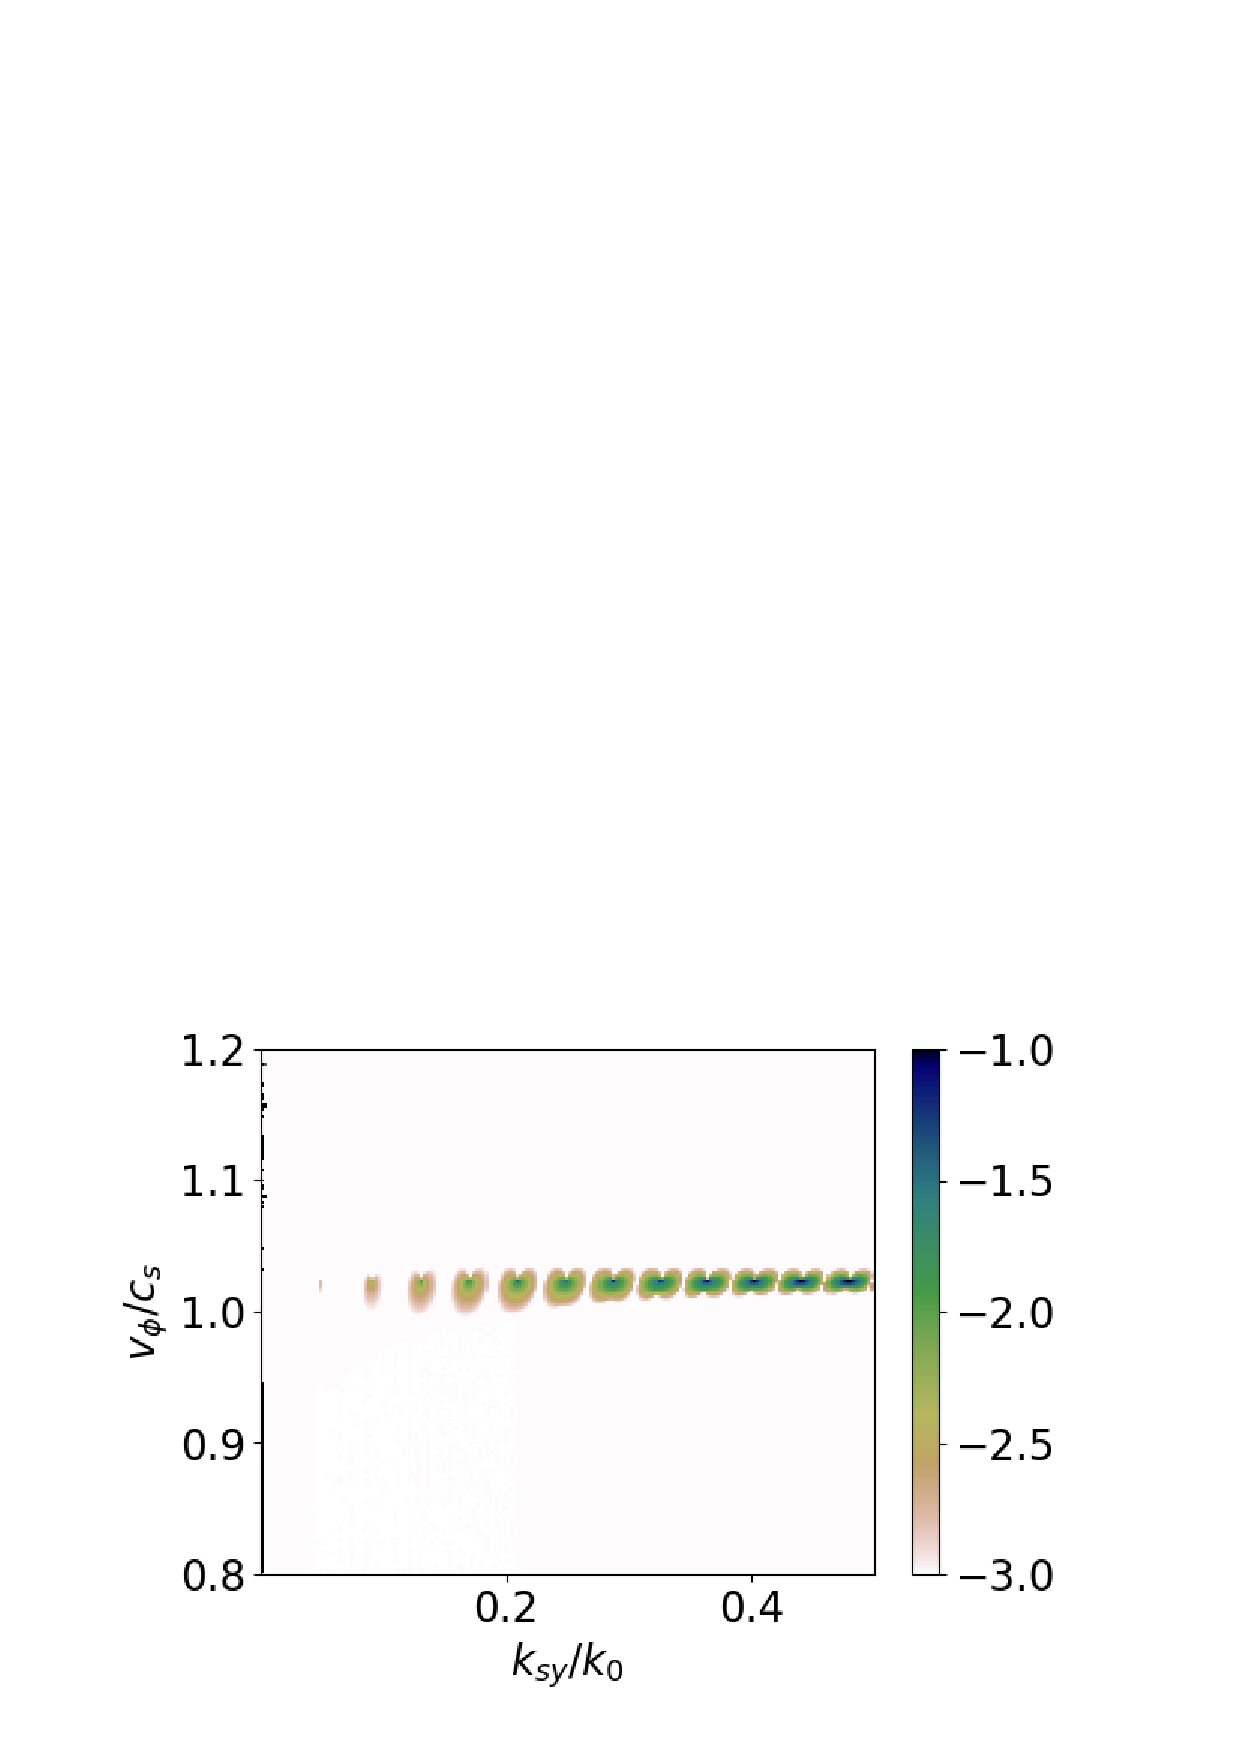
\includegraphics[width=0.24\textwidth]{gkH300.png}&
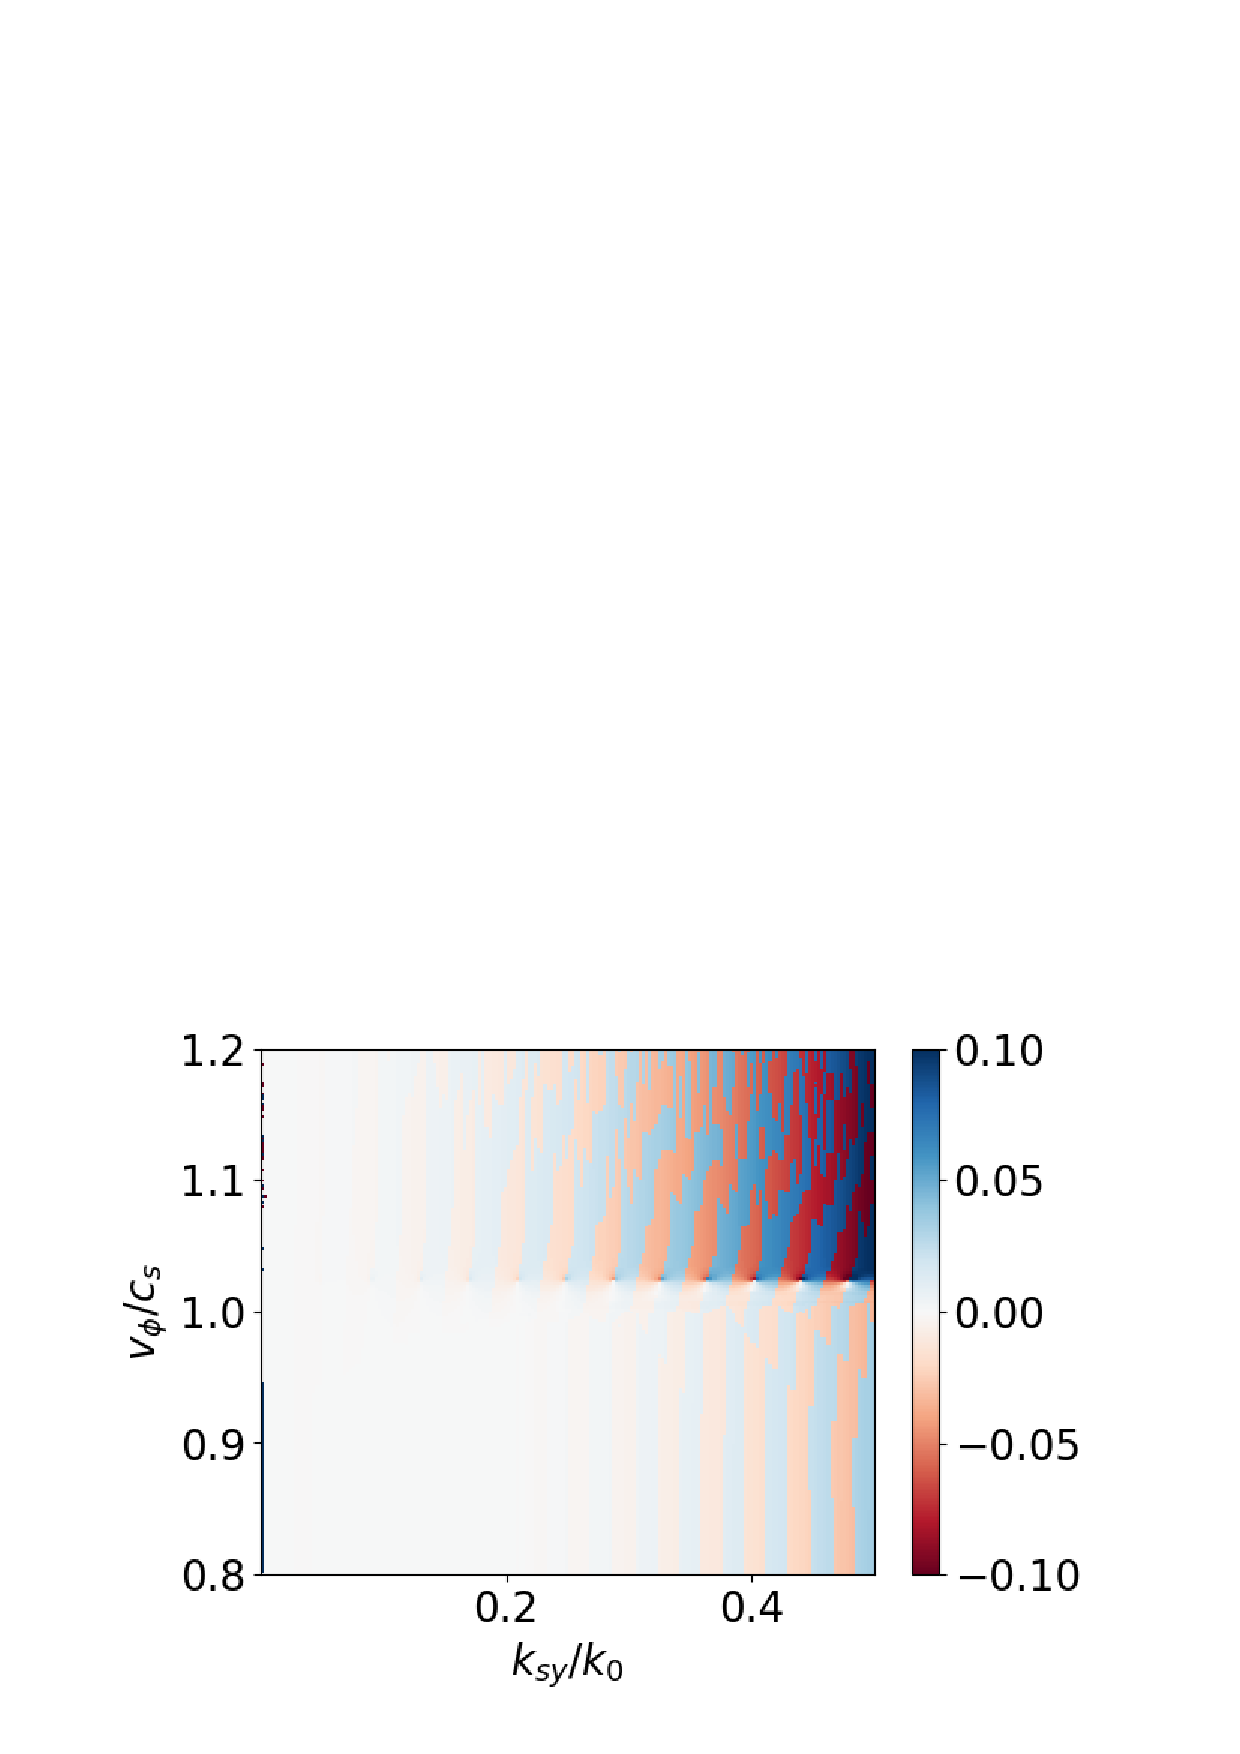
\includegraphics[width=0.24\textwidth]{kkH300.png}\\
(c) Fluid, $\log_{10}(\Gamma/k_0)$  &
(d) Fluid, $\Re(k_{sx}/k_0)$  \\
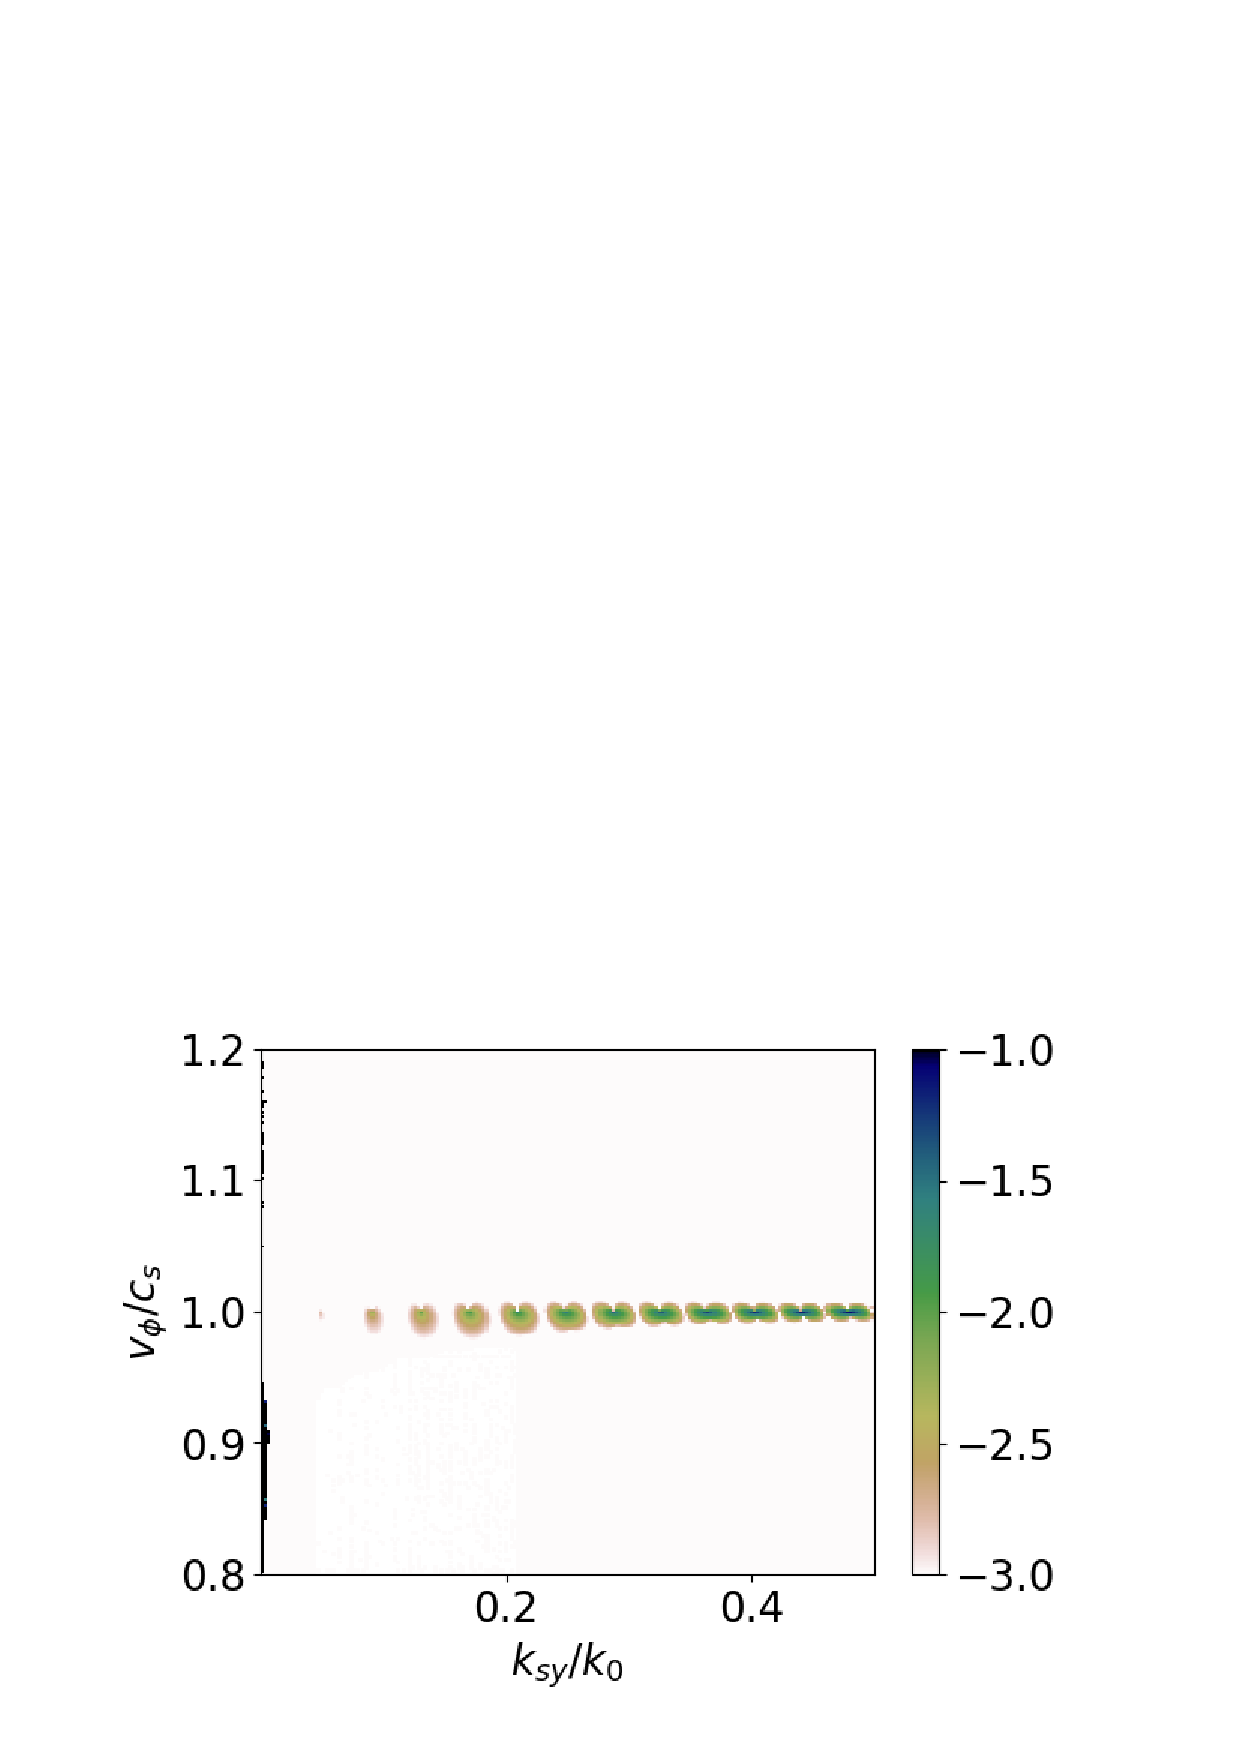
\includegraphics[width=0.24\textwidth]{gfH300.png}&
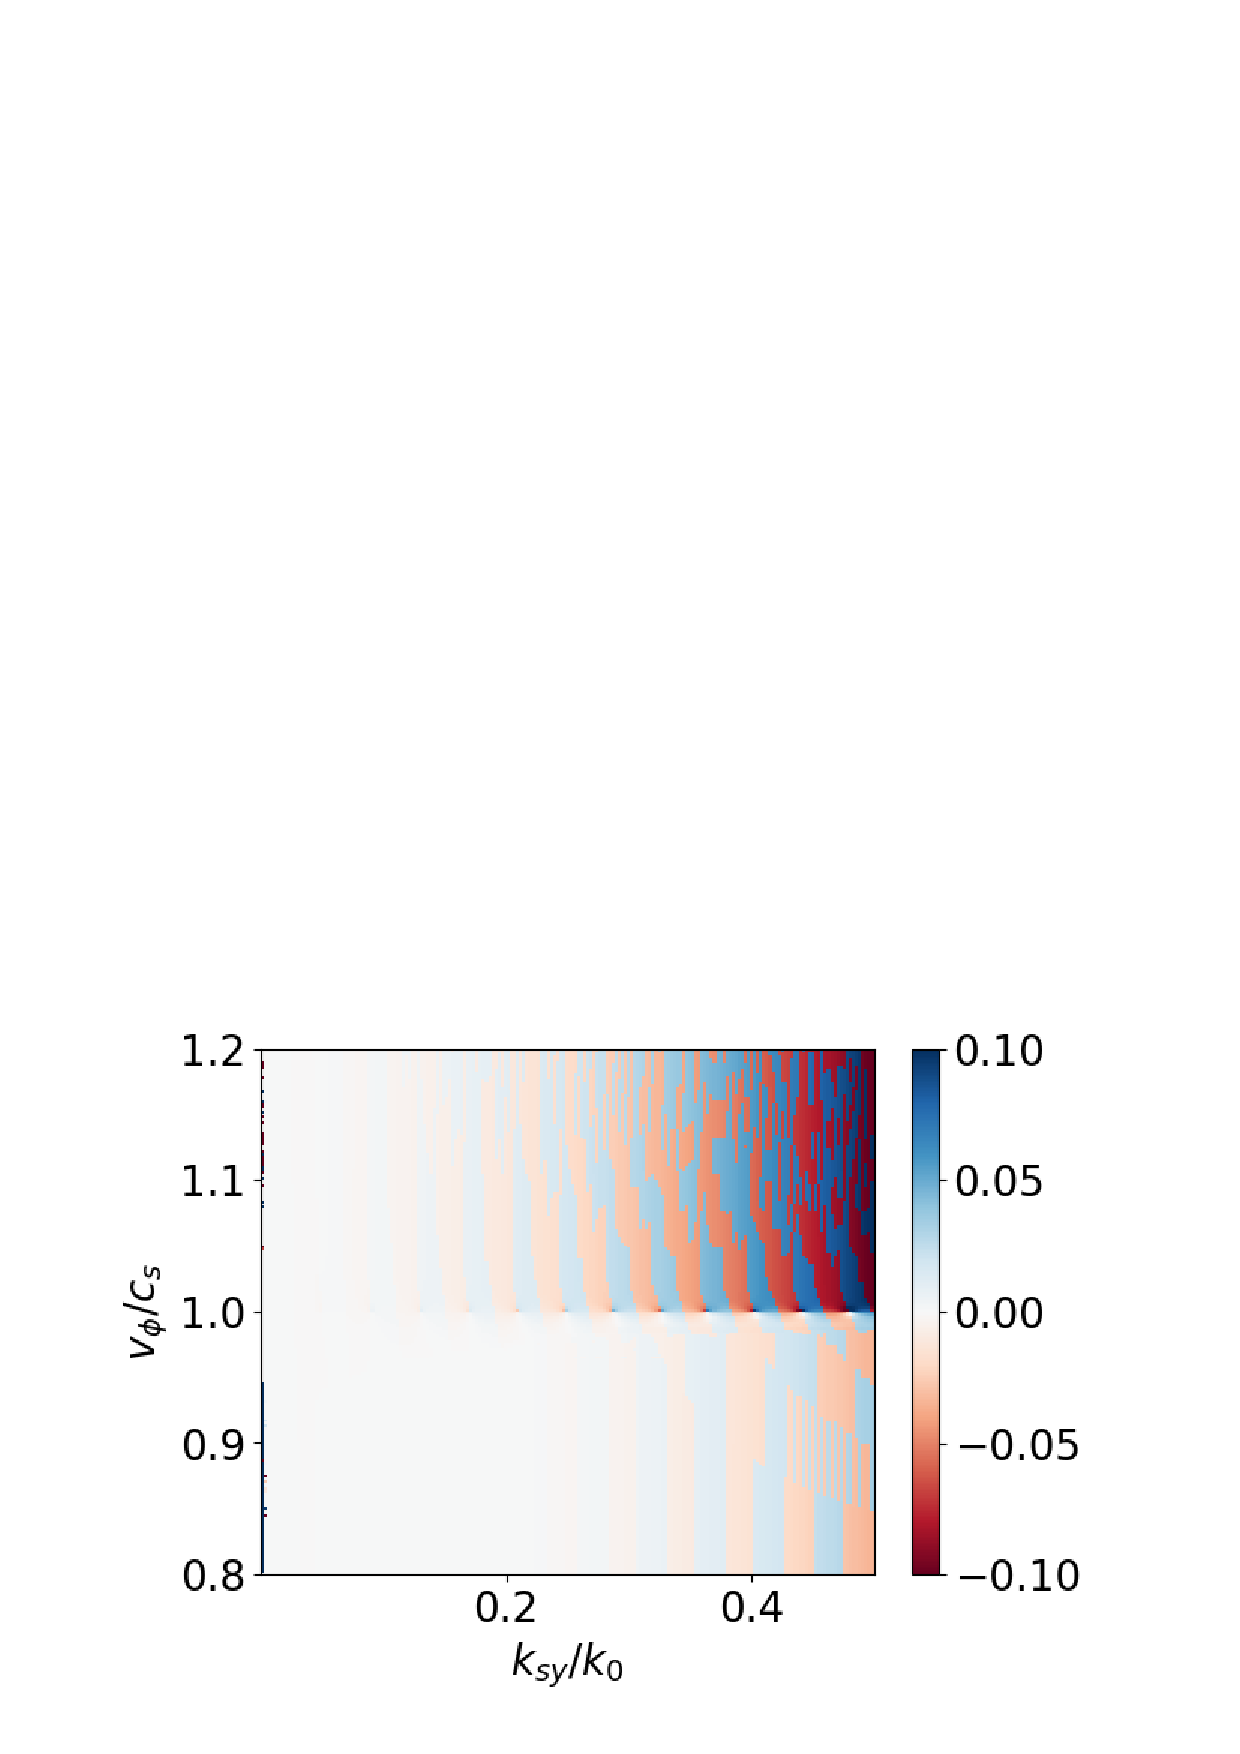
\includegraphics[width=0.24\textwidth]{kfH300.png}
\end{tabular}
\caption{ \label{fig:disperpp}  
Kinetic (a,b) and fluid (c,d) resolution of Eqs. \eqref{eq:dispe2polyrpp}-\eqref{eq:dispe2polyrpp2} for  the same parameters than in Fig. \ref{fig:dispe} assuming a RPP beam given by Eq. \eqref{eq:erpp} with $f_\sharp=8$. The thermal correction of Eq. \eqref{eq:nl} verifies $A_k\le 0.65$ for $k_{sy}\ge 0.1k_0$.
 }
\end{figure}
\begin{figure}
\begin{tabular}{cc}
(a) Kinetic, $\log_{10}(\Gamma/k_0)$ &
(b)  Kinetic, $\Re(k_{sx}/k_0)$ \\
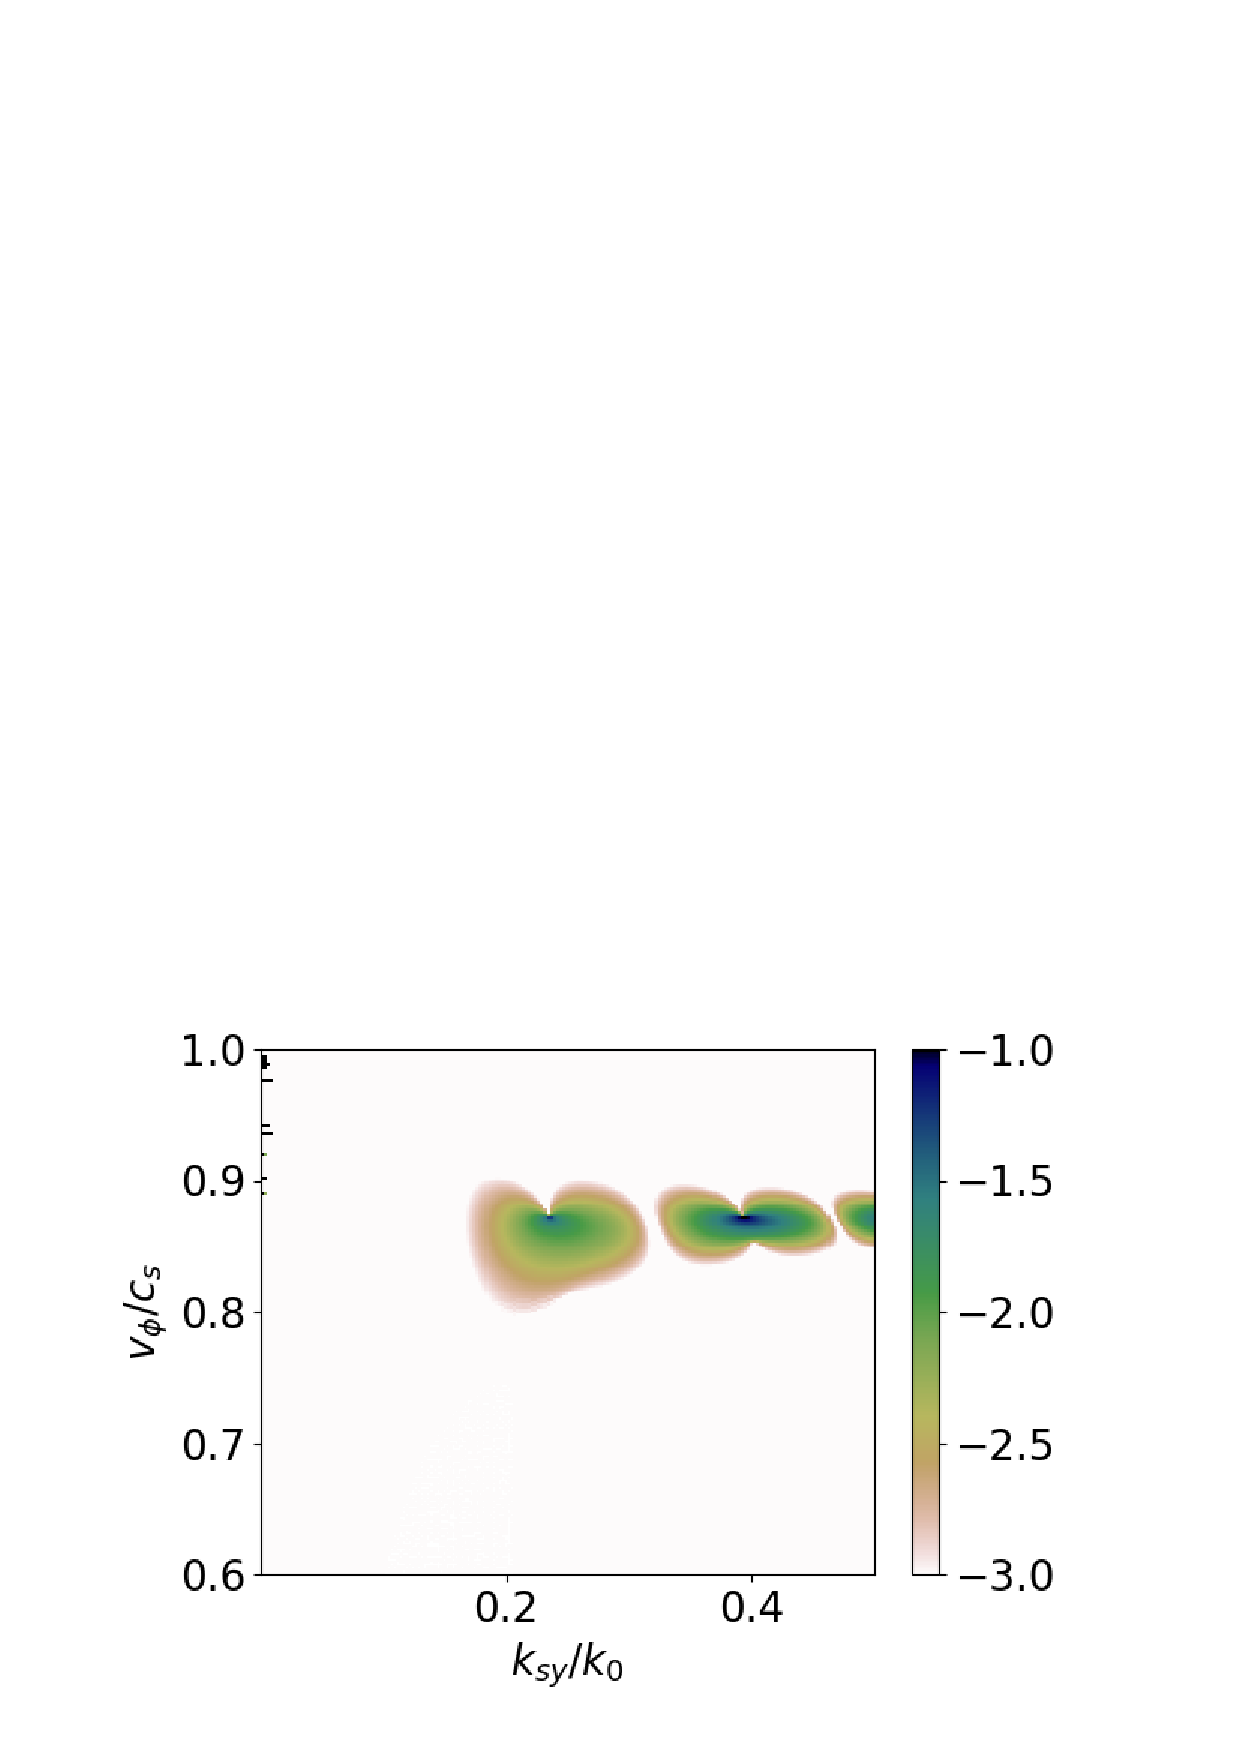
\includegraphics[width=0.24\textwidth]{gkCH.png}&
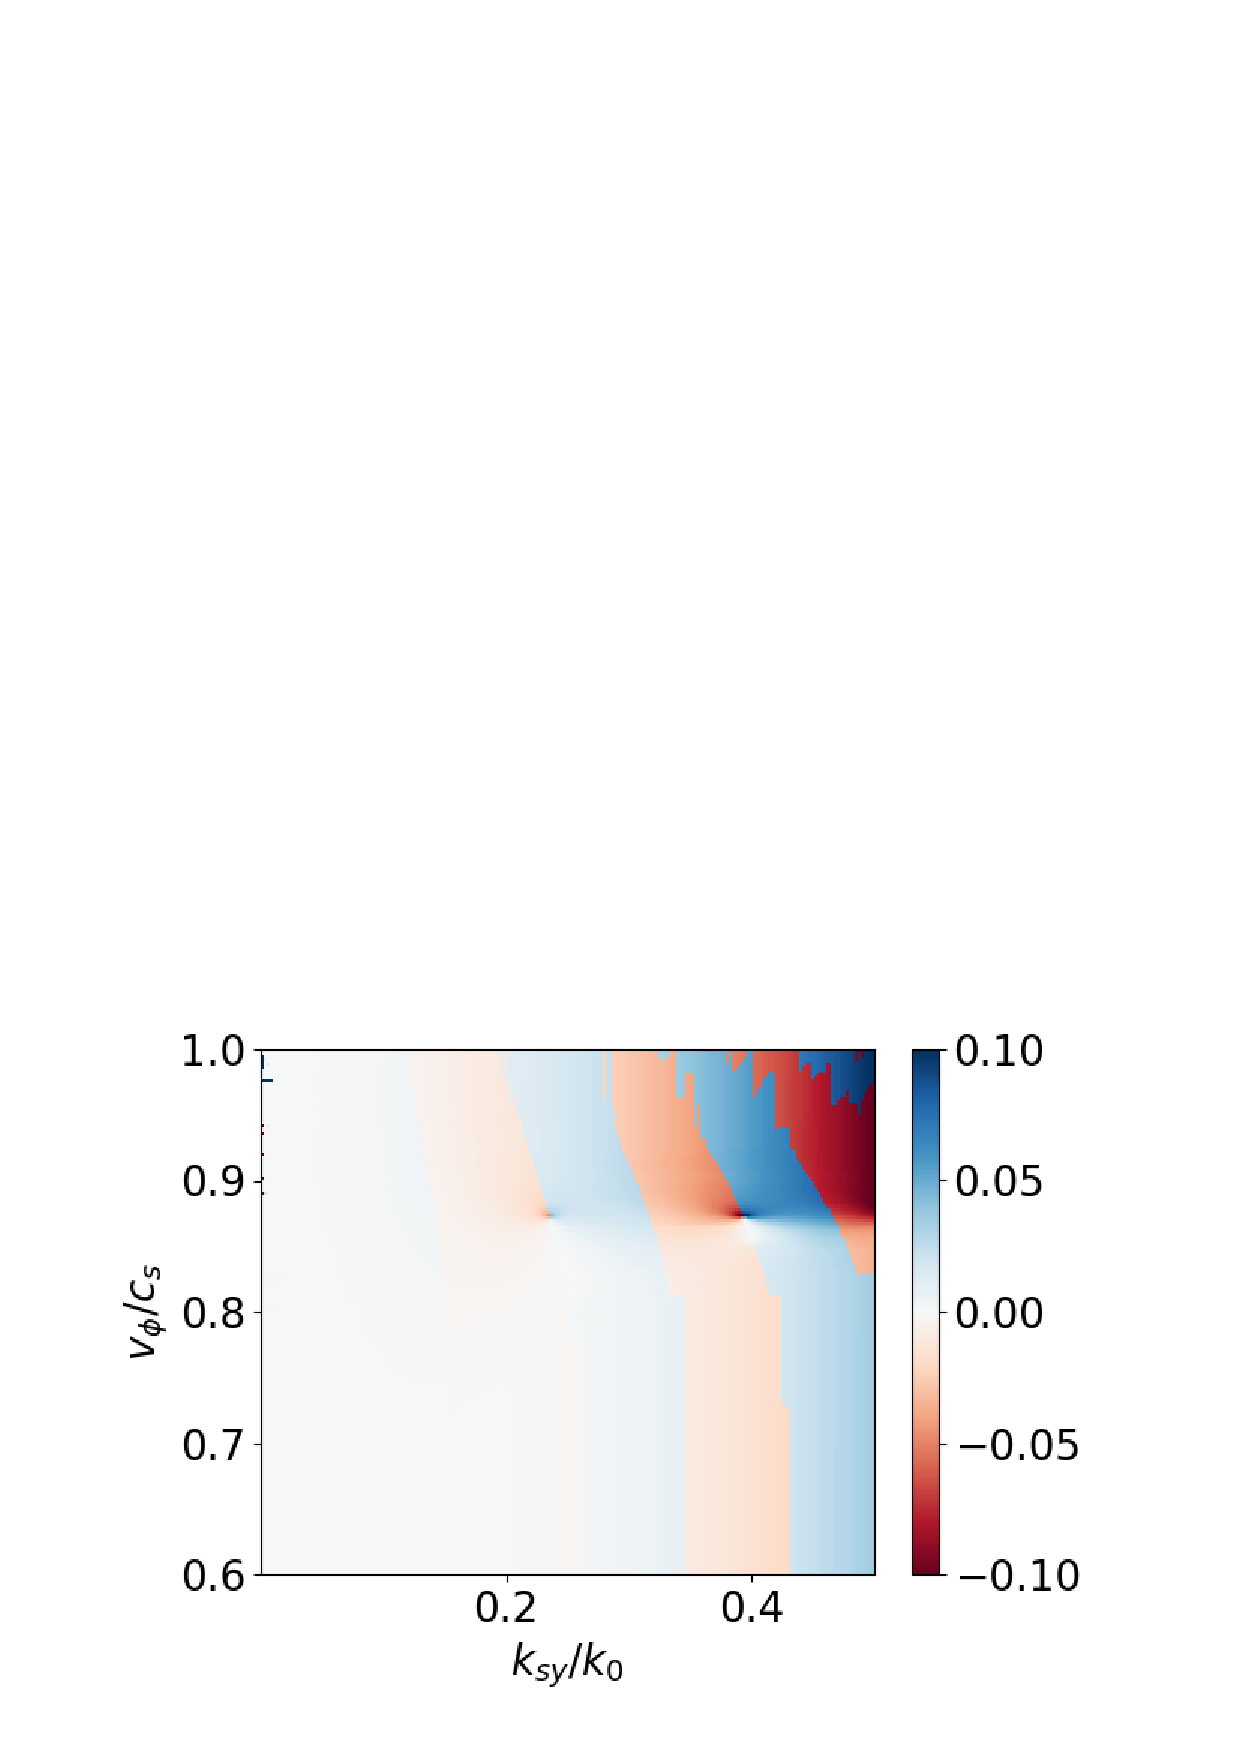
\includegraphics[width=0.24\textwidth]{kkCH.png}\\
(c) Fluid, $\log_{10}(\Gamma/k_0)$  &
(d) Fluid, $\Re(k_{sx}/k_0)$  \\
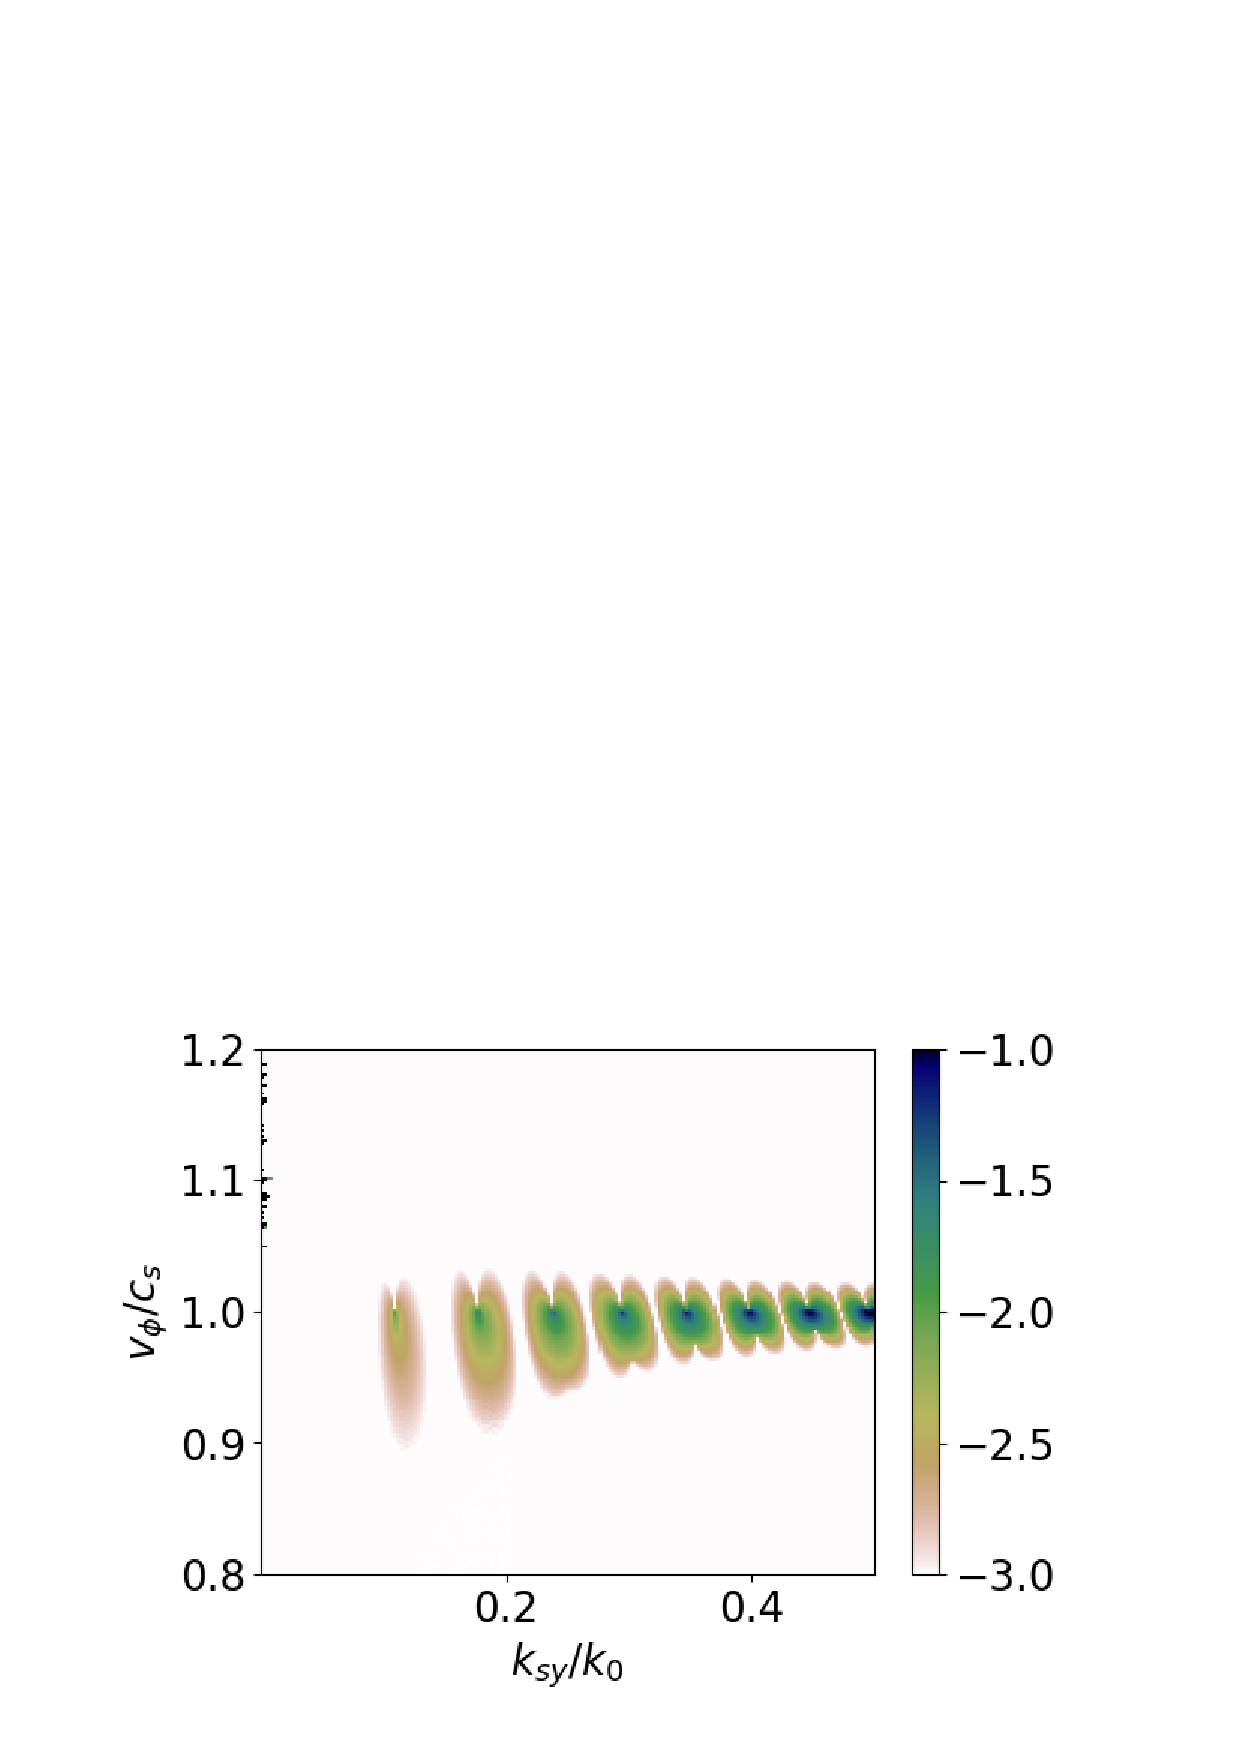
\includegraphics[width=0.24\textwidth]{gfCH.png}&
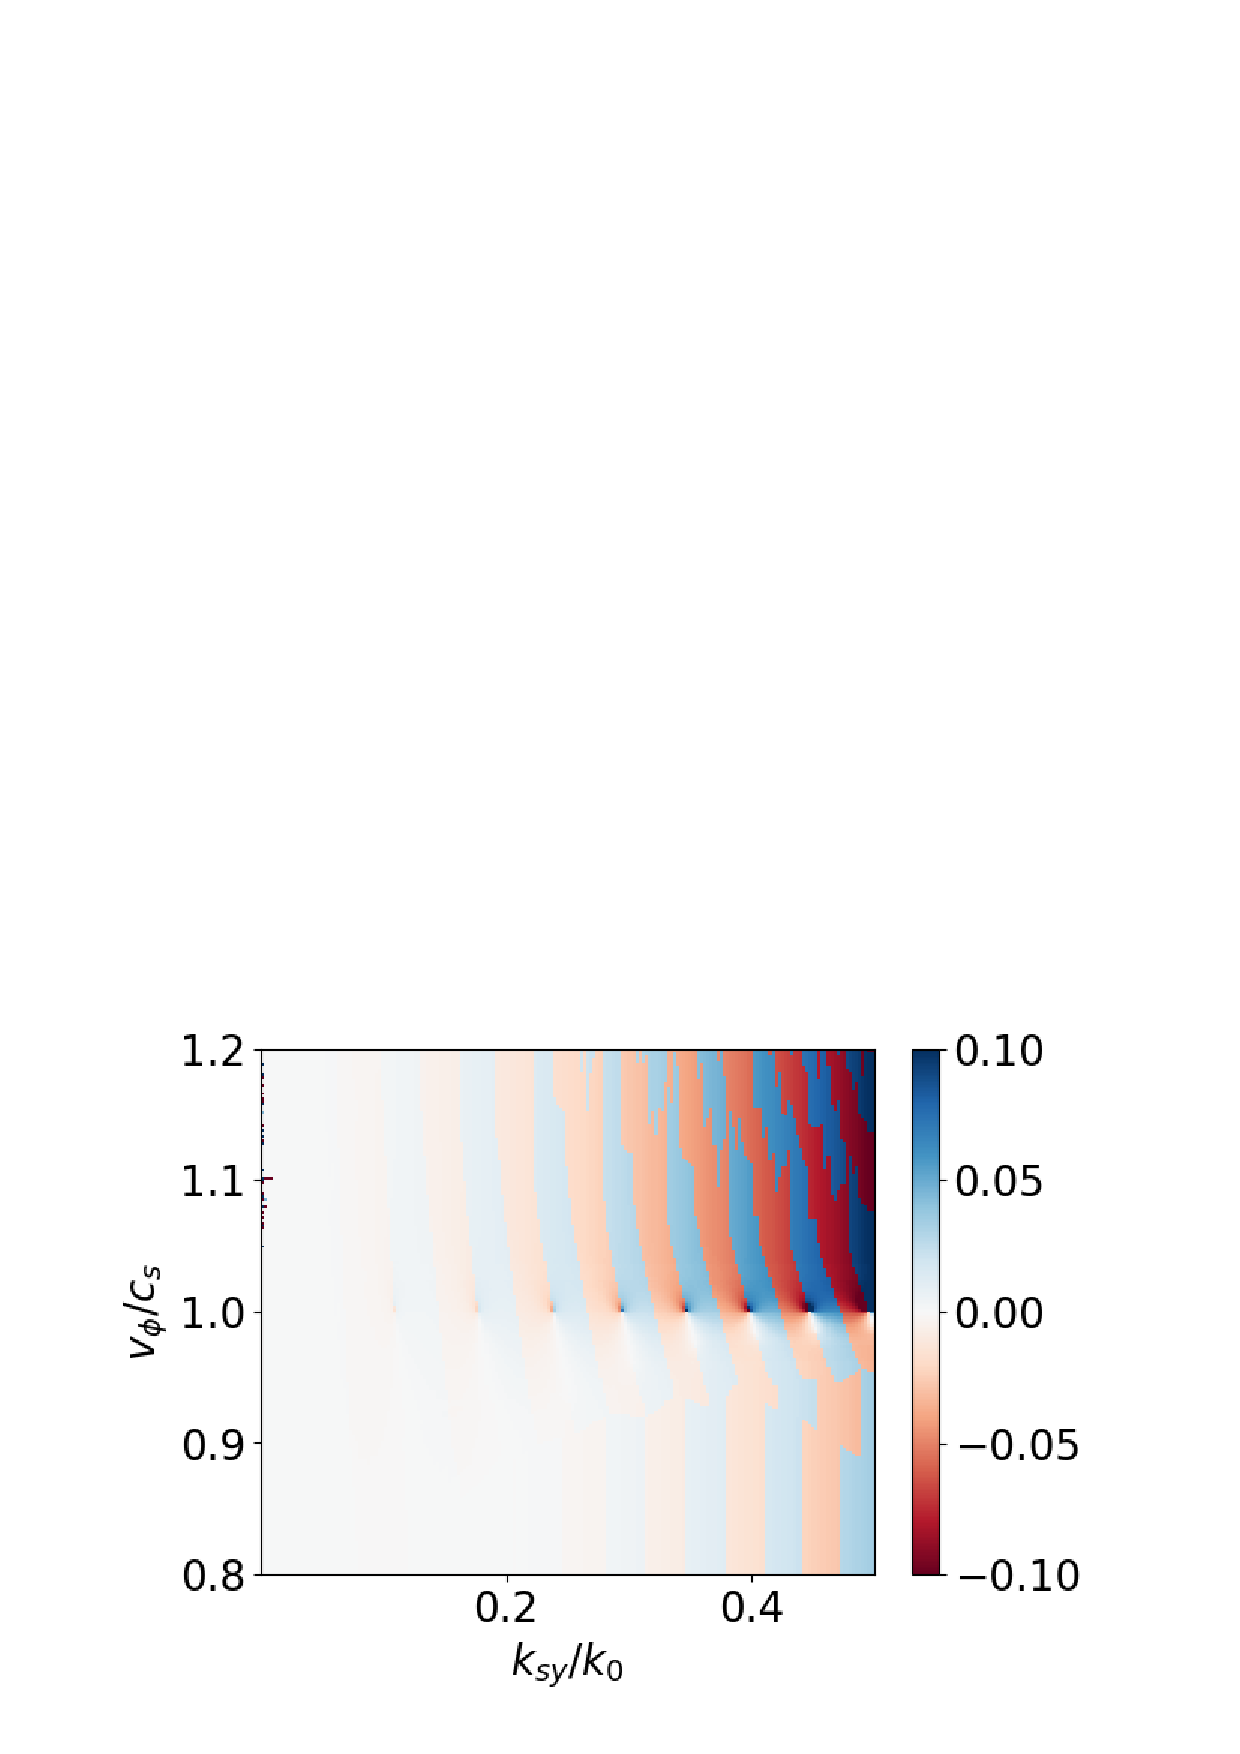
\includegraphics[width=0.24\textwidth]{kfCH.png}
\end{tabular}
\centering{(e) lineout at $v_\phi=0$}\\
\centering{
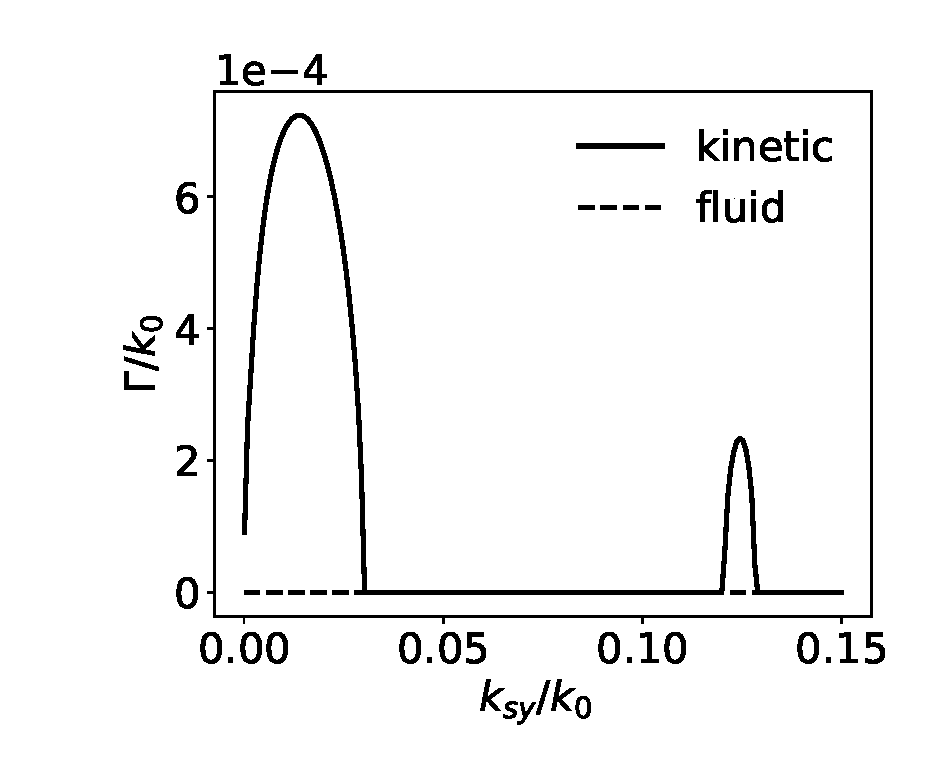
\includegraphics[width=0.24\textwidth]{Fig4e.eps}
}
\caption{ \label{fig:dispeCHrpp}  
Kinetic (a,b) and fluid (c,d) resolution of Eqs. \eqref{eq:dispe2polyrpp}-\eqref{eq:dispe2polyrpp2} for  the same parameters than in Fig. \ref{fig:dispeCH} assuming a RPP beam given by Eq. \eqref{eq:erpp} with $f_\sharp=8$.  The value of the non-local correction [Eq. \eqref{eq:nl}], is obtained with the carbon parameters, corresponding to the smallest electron-ion mean-free-path  and  verifies $A_k\le 1.4$ for $k_{sy}\ge 0.1k_0$. Use is made of the mean charge number and mean mass number for calculating the sound speed and the normalized Landau damping rate $c_s$ and $\gamma_0$.
Panel (e) corresponds to lineouts at $v_\phi=0$  of  (a) and (c). 
 }
\end{figure}
In order to finalize the RPP dispersion relation, we will proceed to a statistical averaged using Eq. \eqref{eq:d}. On the right-hand-side,  $\langle\exp(-i\Phi_{k_1}+i\Phi_{k_2})\delta n_e \rangle$ can be recast as
\begin{equation}
\langle\exp(-i\Phi_{k_1}+i\Phi_{k_2})\delta n_e \rangle= \langle\exp(-i\Phi_{k_1}+i\Phi_{k_2}) \rangle\langle\delta n_e \rangle + \mathcal{C}\, , \label{eq:mthcalc}
\end{equation}
where $\mathcal{C}$ is the correlations   between  \mbox{$\exp(-i\Phi_{k_1}+i\Phi_{k_2})$} and $\delta n_e$. The combination of Eq. \eqref{eq:fddrpp} with \eqref{eq:mthcalc} shows that $\mathcal{C}\propto \delta n_0/n_c$ and therefore, to leading order in $\delta n_0/n_c$, $\mathcal{C}$ may  be neglected when  averaging   Eq. \eqref{eq:fddrpp}, giving
\begin{align}
  1= -\alpha_{k/f}(v_\phi)A_k \frac{\delta n_0}{n_c} \frac{\omega_0^2}{N}\sum_{ k_{1} }        \left[ \frac{1 }{D_-(k_{1})} +\frac{1}{D_+(k_{1})} \right] \, .\label{eq:disperpp} 
\end{align}
Provided the phase plate has a sufficient number of elements (\emph{i.e.} $N$ is large enough), we shall replace the discrete sum by a continuous one. 
\tc{Although the neglect of  $1/D_+$ in the above equation is usual regarding the Brillouin parametric instabilities, both  $1/D_\pm$ are found here to be important for  quantitatively describing the forward Brillouin scatter. }
To leading order 
in  $\omega_s\ll\omega_0$, and making use of the pump wave dispersion relation, $\omega_0^2=\omega_{pe}^2+k_0^2c^2+k_1^2c^2$,
\begin{equation}\label{eq:dpmk1}
D_\pm(k_1) \simeq -\mathbf{k}_s^2c^2\pm 2(\omega_s\omega_0 - k_{sx}k_0 c^2-k_{sy} k_1 c^2) \, , 
\end{equation} 
so that,
\begin{align}
 \frac{1}{N} \sum_{ k_{1} }  \frac{1 }{D_\pm(k_{1})}  \simeq \frac{1}{2k_m} \mathrm{P.V.} \int_{ -k_m }^{ k_m }       \frac{dk_1 }{D_\pm(k_{1})}  \, , \nonumber\\
 \simeq \frac{\mp\,1}{4k_mk_{sy}c^2} \ln\left[
 \frac{ -\mathbf{k}_s^2c^2\pm 2(\omega_s\omega_0 - k_{sx}k_0 c^2-k_{sy} k_m c^2)}{ -\mathbf{k}_s^2c^2\pm 2(\omega_s\omega_0 - k_{sx}k_0 c^2+k_{sy} k_m c^2)} \right] \, .\label{eq:sumint} 
\end{align}
We introduced, $\mathrm{P.V.}\int f$, the principal value of $\int f$.
The combination with Eq. \eqref{eq:disperpp} yields
\begin{align}
 \frac{-4k_mk_{sy}c^2}{\alpha_{k/f}(v_\phi)A_k \omega_0^2\delta n_0/n_c  } \nonumber\\
 \simeq  \ln\left[
 \frac{ (\mathbf{k}_s^2c^2-2k_{sy} k_m c^2)^2 -4(\omega_s\omega_0 - k_{sx}k_0 c^2)^2}{ (\mathbf{k}_s^2c^2+2k_{sy} k_m c^2)^2 -4(\omega_s\omega_0 - k_{sx}k_0 c^2)^2} \right] \, .\label{eq:disperpp2} 
\end{align}
In order to avoid the branch cuts of the complex logarithm, it is convenient to recast the dispersion relation into 
\begin{align}
u^2 -2\frac{v_\phi}{\eta c}u +\frac{v_\phi^2}{\eta^2 c^2}-\frac{1}{4}A =0 
\, , \label{eq:dispe2polyrpp} \\
A= \frac{1}{1-B}\left[ \left(\frac{k_{s}^2}{\vert k_{s}\vert k_0}-\frac{k_{sy}}{\vert k_{s}\vert f_\sharp}\right)^2-\left(\frac{k_{s}^2}{\vert k_{s}\vert k_0}+\frac{k_{sy}}{\vert k_{s}\vert f_\sharp}\right)^2B  \right]\, , \label{eq:dispe2polyrpp1}  \\ 
B =\exp\left(\dfrac{-4k_m  k_{sy}c^2}{\alpha_{k/f}(v_\phi)A_k \omega_0^2\delta n_0/n_c  }\right)\, .
\label{eq:dispe2polyrpp2} 
\end{align}
Note that the dependence of $A$ on $k_{sx}$ may be neglected (provided  $\vert k_{sx}\vert \ll \vert \mathbf{k}_s\vert$)  so that  $u =  k_{sx}/\vert \mathbf{k}_s\vert$  may verify  a second order polynomial equation given by Eq. \eqref{eq:dispe2polyrpp} with
\begin{align}
A\simeq \frac{1}{1-B}\left[ \left(\frac{\vert k_{s}\vert}{k_0}-\frac{1}{f_\sharp}\right)^2-\left(\frac{\vert k_{s}\vert}{k_0}+\frac{1}{f_\sharp}\right)^2B  \right]\, , \label{eq:dispe2polyrpp1_lin}  \\ 
B \simeq \exp\left(\dfrac{-4k_m \vert k_{s}\vert c^2}{\alpha_{k/f}(v_\phi)A_k \omega_0^2\delta n_0/n_c  }\right)\, .
\label{eq:dispe2polyrpp2_lin} 
\end{align}
The only difference between the plane wave and the RPP dispersion relations holds in the last term of the l.h.s. of Eqs. \eqref{eq:dispe2poly} and \eqref{eq:dispe2polyrpp}. 
As expected,  the latter coincide when  a Taylor expansion of $A$ [Eq. \eqref{eq:dispe2polyrpp1_lin}] to first order  in $1/f_\sharp$ is done, \emph{i.e.} for a vanishing  RPP beam spectral width, $2k_m=k_0/f_\sharp$.
Care has been taken to verify that the RPP dispersion relations with  $f_\sharp \ge 50$ yield  very similar results than Eq. \eqref{eq:dispe2poly}. 
We also verified that extracting $k_{sx}$ from a numerical resolution of Eq. \eqref{eq:disperpp} also yields similar results for $100$ phase plate elements (\emph{i.e.} when the sum runs over $N=100$ regularly spaced elements of $[-k_m,k_m]$).


%They have been obtained by retaining the growing part of both solutions of Eq. \eqref{eq:dispe2polyrpp}.
%
The solutions of the RPP dispersion  equations \eqref{eq:dispe2polyrpp}-\eqref{eq:dispe2polyrpp2} stem from a non linear algebraic solver, or using a dichotomous algorithm applied at fixed  $v_\phi$ and starting from low values of $\vert \mathbf{k}_s\vert$. The initial guess is  seeded by the approximated solutions of Eqs. \eqref{eq:dispe2polyrpp}, \eqref{eq:dispe2polyrpp1_lin} and  \eqref{eq:dispe2polyrpp2_lin}, yielding convergence toward the exact solution. Moreover, if $k_x(\omega_s, k_y)$ is a solution of Eq.  \eqref{eq:disperpp2},  the symmetry properties of our free-drift velocity  dispersion relations imply that  
$-k_x(-\omega_s, k_y)$ and $k_x^\star(-\omega_s, k_y)$ are also solutions (where $z^\star$ is the complex conjugate of $z$), therefore  helping to constrain the numerical solver to converge toward a single eigenmode. The spatial growth rate and wavevector longitudinal component are illustrated in  
Figs. \ref{fig:disperpp} and \ref{fig:dispeCHrpp} with identical plasma and laser parameters than in Figs.  \ref{fig:dispe} and \ref{fig:dispeCH}, respectively and with $f_\sharp=8$. Finally, the assumption made in deriving Eqs. \eqref{eq:dispe2polyrpp1_lin}-\eqref{eq:dispe2polyrpp2_lin} ($\vert k_{sx}\vert \ll \vert \mathbf{k}_s\vert$) seems, for the parameters of interest here, scarcely verified (see Figs. \ref{fig:disperpp} and  \ref{fig:dispeCHrpp} where for  $k_{sy}/k_0=0.4 $, $\vert k_{sx}\vert/k_0$ reaches $\sim 0.1$).

Hence, regarding the FSBS, no simple stability criterion could be extracted from our dispersion relation such as the one proposed in Refs. \cite[]{Lushnikov_2006,phd-Grech,PRL_Grech_2009}.
Figures \ref{fig:disperpp}(b,d) and \ref{fig:dispeCHrpp}(b,d) also suggest that, in contrast with the plane wave case, the FSBS growing of a RPP beam induces acoustic fluctuations which propagating direction may  have a finite $x$ component.

\subsection{Filamentation of a spatially smoothed beam}\label{sec:filam}
Regarding the H$^+$-plasma case (Fig. \ref{fig:disperpp}), the propagation of the smoothed beam is, as expected  \cite[]{NatPhys_Glenzer,POP_Berger_98b,PRL_Sarri_2011}, stable regarding the filamentation instability, \emph{i.e.} no growth is obtained  at $v_\phi=0$. In that case, Eq. \eqref{eq:dispe2polyrpp} simplifies to $u^2=A/4$ which can be recast into a second order polynomial equation in $k_{sx}^2$,
\begin{align}
    k_{sx}^4 + z_2 k_{sx}^2 +z_0=0 \, ,\nonumber \\
    z_2 = 2k_0^2\left(  \frac{k_- -k_+ B}{k_0(1-B)} -2  \right)\, , \nonumber\\
    z_0 = k_0^2\frac{k_-^2 -k_+^2 B}{(1-B)}\, ,\nonumber \\
    k_\pm =\frac{k_{sy}^2}{k_0}\pm\frac{k_{sy}}{f_\sharp} .\label{eq:dispefilam}
\end{align}
The unstable solution of the above equation is purely imaginary and corresponds to the spatial growth rate of a spatially smoothed laser filamentation instability.
Physically, the speckle typical size, $f_\sharp\lambda_0$, remains smaller than the most unstable filamentation wavelength [$\sim 10 \,\rm\mu m$ in Fig. \ref{fig:dispe}(a)] thus preventing the transverse standing electrostatic wave to grow. The artificial increase of $f_\sharp$ in excess of $\sim 25$, \emph{i.e.} yields a finite value of the filamentation spatial growth rate as the speckle size starts to be comparable with the plane wave most unstable wavelength. 
For more moderate  $f_\sharp$-numbers, the propagation of a laser may  also remains filamentation-unstable, despite the use of random phase plates,  in  the case of a multi-ion species plasmas such as in Fig.   \ref{fig:dispeCHrpp}. 
Although less filamentation unstable than in the plane wave case [see Figs. \ref{fig:dispeCH}(a,c) and \ref{fig:dispeCHrpp}(e)], the RPP beam has a finite kinetic growth rate maximized at  $\Gamma\sim 7\times 10^{-4}k_0 $  and $\vert k_s\vert \sim  10^{-2}k_0$. 
Hence, the estimated  gain of $\sim 12$   for a millimeter of propagation (with a wavelength of $\sim 35 \,\rm \mu m$) indicates that keV-range plasmas may produce significant RPP-laser filamentation, at least in the multi-ion species case.
Unfortunately, the use of random phase plates seems to completely stabilize the filamentation in the fluid framework [see dashed line, Fig. \ref{fig:dispeCHrpp}(e)], demonstrating that  hydrodynamic codes fail to capture correctly the laser filamentation in a multi-ion species plasma. \tc{The only difference between the two frameworks comes from the plasma response factor [Eqs. \eqref{eq:alphak}-\eqref{eq:alphaf}] which reads $\alpha_{f}(v_\phi=0)=0.62$ and $\alpha_{k}(v_\phi=0)=0.88$, thus demonstrating that low $Z_iT_e/T_i$ multi-ion species plasmas are more prone to hole boring than their often used fluid averaged-ion  approximate. } 
Additionally, the kinetic instability characterized in Fig. \ref{fig:dispeCHrpp}(e)  is mainly thermal as \tc{ the growth rate vanishes} when   replacing  $A_k$ in Eq. \eqref{eq:dispefilam} by its collisionless value, $1/2$. 

Notably, another filamentation mode exists around  $\vert k_s\vert \simeq 2k_0/(2f_\sharp) = 0.125k_0$, albeit with a smaller growth rate $\Gamma\sim 2\times 10^{-4}k_0 $. \tc{This feature corresponds to the speckle-scale filamentation and, as it is sub-dominant, seems to cast doubts on the validity of hot-spot power thresholds \cite[]{POF_Max_1976,POP_Williams_2006} regarding the large-wavelength thermally driven  filamentation growth evidenced in Fig.   \ref{fig:dispeCHrpp}(e).}

\subsection{Comparison with proton radiographs of a RPP pulse propagating in a helium gaz jet}\label{sec:xp}
\begin{figure}
(a) Setup \\
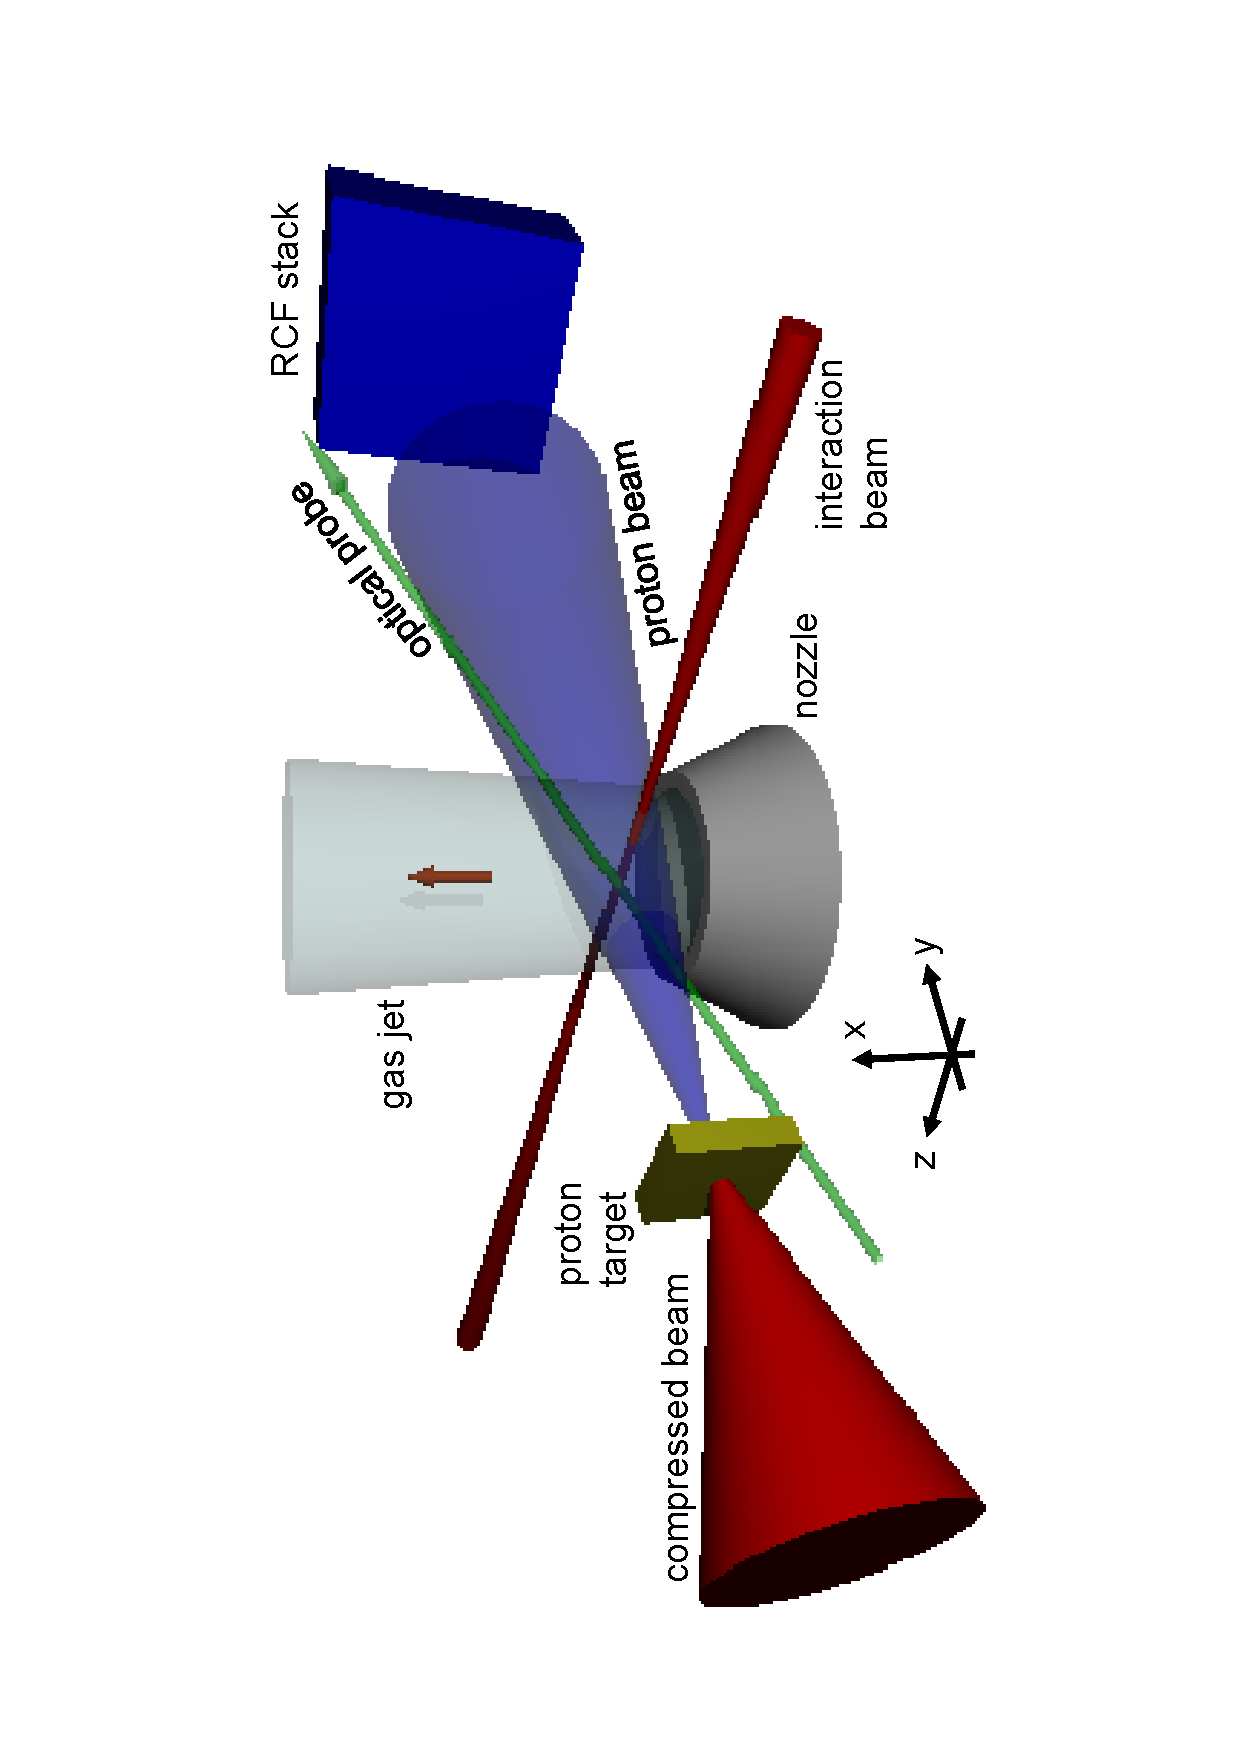
\includegraphics[width=0.4\textwidth,angle=-90]{set_up.pdf}\\
(b) Experimental RCF \\
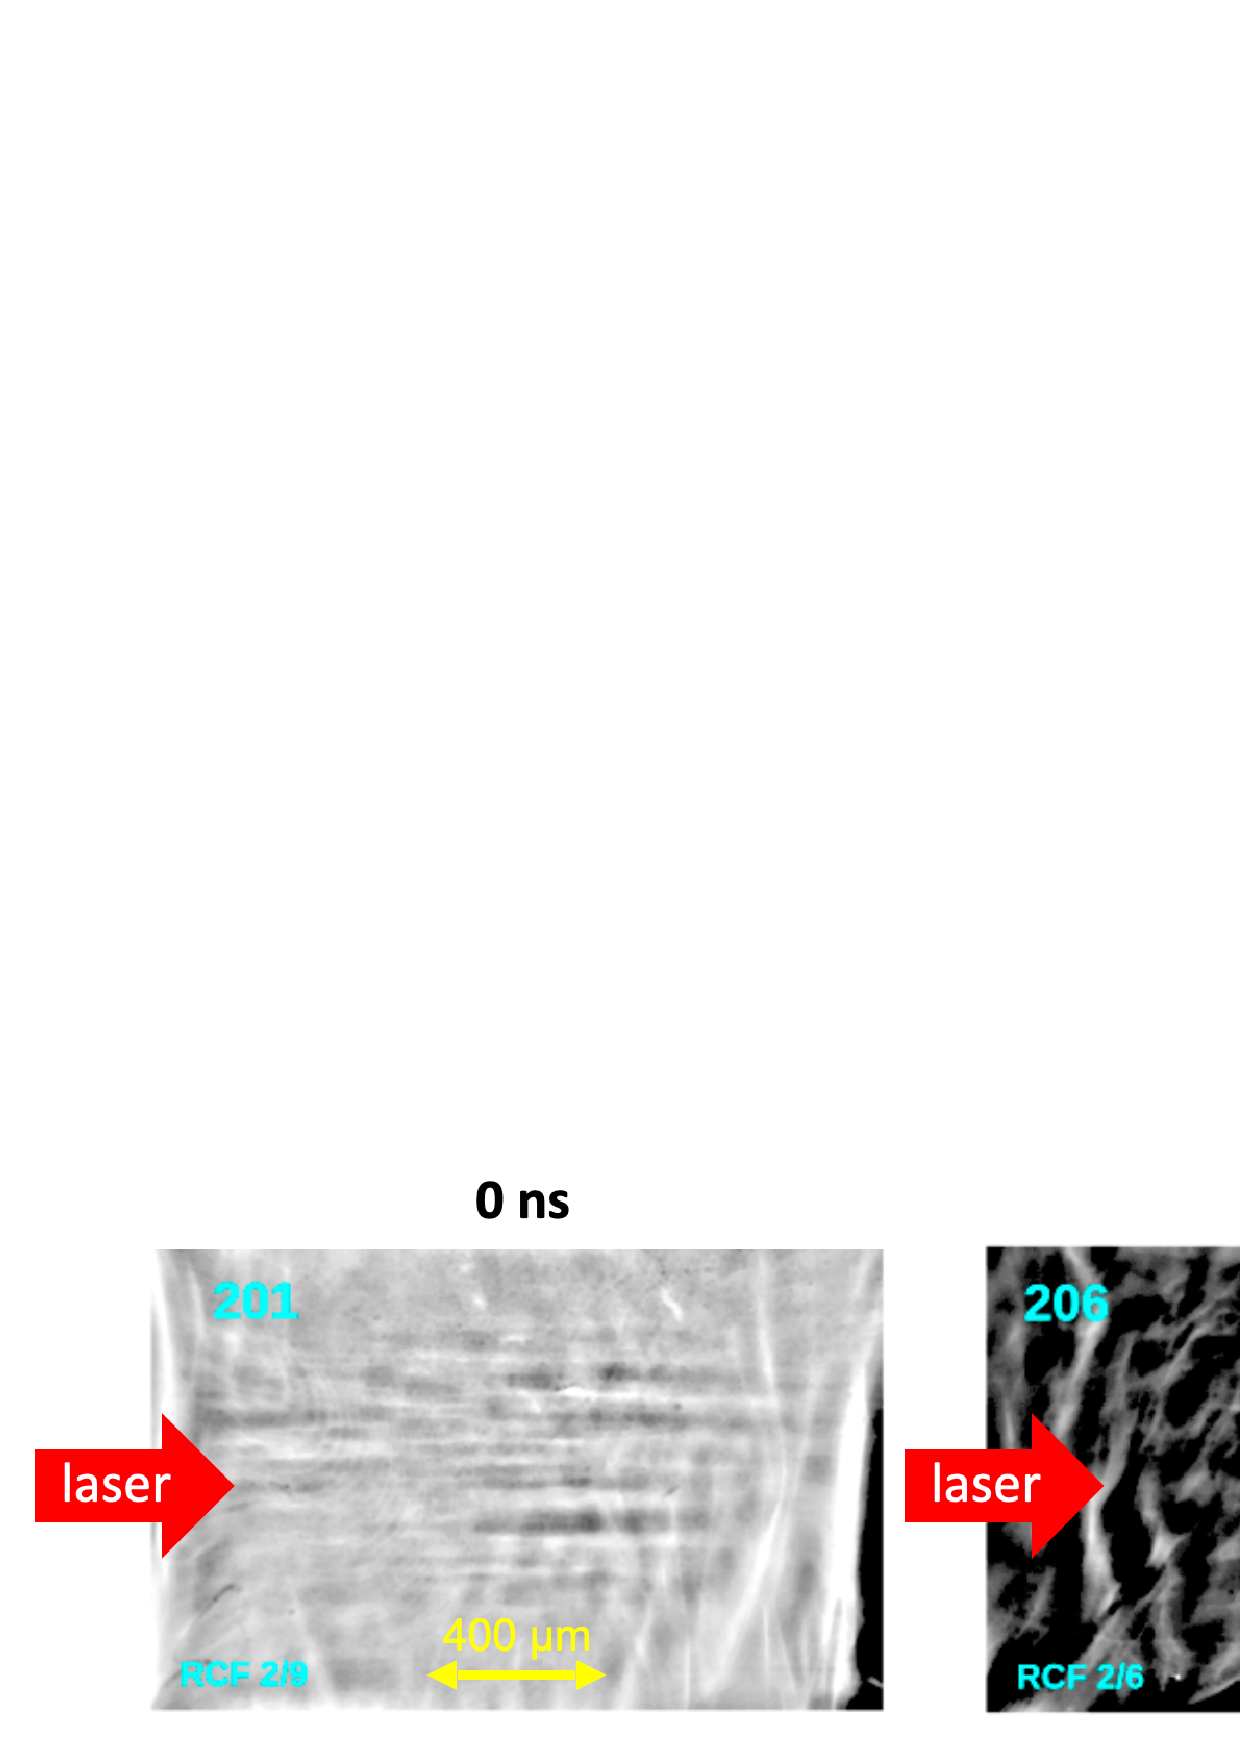
\includegraphics[width=0.45\textwidth]{rcf.png}
\caption{ \label{fig:xpfuchs_xp}  
(a) Sketch of the experimental setup.
(b) Experimental RCF (obtained using 3 MeV protons) from two shots of the LULI experiment, at $0$ and $0.75$ ns after the maximum intensity reaches the center of the plasma slab.  The scale indicated at the bottom of the left image applies to both and refers to the target plane. 
 }
\end{figure}
\begin{figure}
\begin{tabular}{cc}
(a) $T_e(t)$ and $I_0(t)$&
(b) $\Gamma \times L$  \\
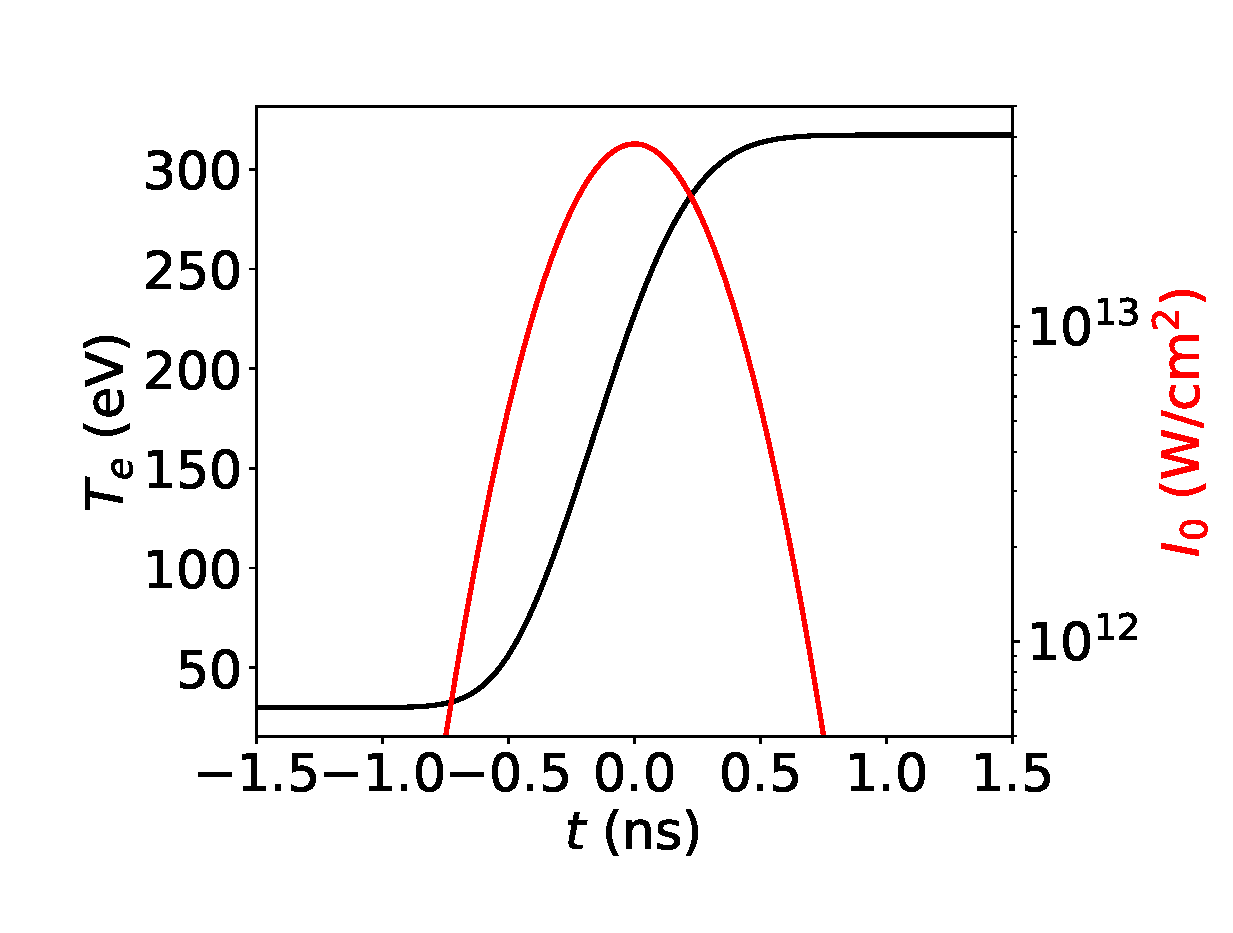
\includegraphics[width=0.245\textwidth]{xp_fuchs_te_new.eps}& 
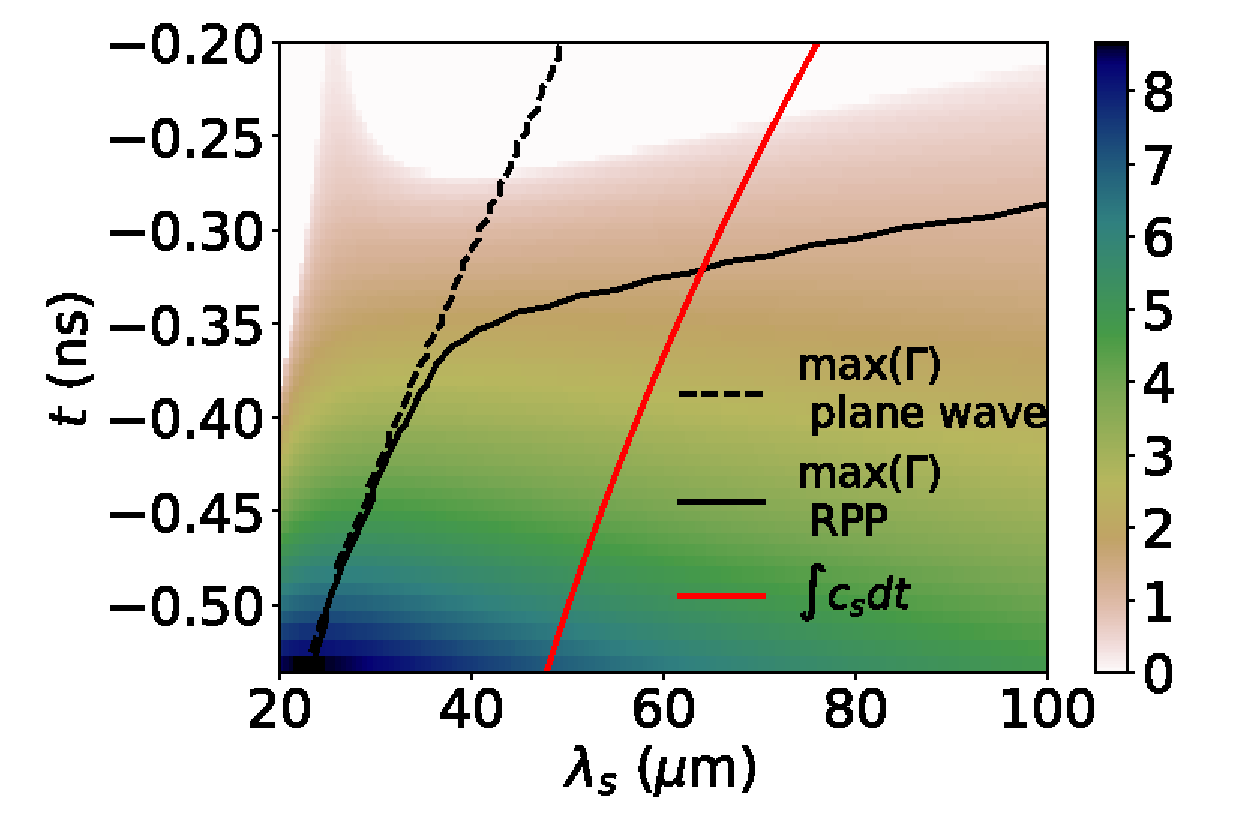
\includegraphics[width=0.24\textwidth]{xp_fuchs_new.eps}
\end{tabular}
\caption{ \label{fig:xpfuchs_th}  
(a) Temporal evolution of the electron temperature 
%from an Hydrodynamic simulation  \tc{with the code HERA} and 
from the resolution of $(3/2)n_e d_tT_e=\nu_BI_02^{-t^2/\tau^2}/c$ with $\tau = 300\,\rm ps$  and $T_e(-1.5 \, \rm{ns})=30\,\rm eV$ (left axis, black).
The intensity evolution is superimposed as a red line (right axis).
(b) Filamentation growth rate corresponding to the unstable solution  of Eq. \eqref{eq:dispefilam} normalized to the plasma length  $L$  for $v_\phi=0$ and in the fluid framework [Eq. \eqref{eq:alphaf}] with $I_0=3.8\times 10^{13}\, \rm W/cm^2$, $2\pi/k_0=1\,\rm\mu m$, $f_\sharp=24$, $Z_i=2$, $A=4$, $n_e=10^{19} \,\rm cm^{-3}$,  $L=1\,\rm mm$ and  $Z_iT_e/T_i=\tc{5}$. 
The growth rate maximum is superimposed as a  black line in the RPP case and as a dashed line in the plane wave case [Eq. \eqref{eq:dispe2poly}].
 }
\end{figure}

A low temperature plasma may also be filamentation-unstable to the  propagation of a RPP pulse.
For a single ion species plasma, and provided $Z_iT_e\gg T_i$,   we recall that $\alpha_f(0)=1\simeq \alpha_k(0)$, for this reason, the filamentation growth coincides in both  kinetic and hydrodynamic frameworks. 
Hence, restricting, in this section, the analysis to the fluid plasma response, we aim at comparing our predictions with the laser filamentation observed experimentally at relatively low temperature.

The experiment, detailed in Ref. \cite[]{PRL_Sarri_2011}, uses a tightly focused ($f_\sharp =3$) RPP pulse,  therefore probably out of reach of our dispersion relations where we neglected diffraction  on the pump wave envelope [in Eq. \eqref{eq:erpp}].
Hence the choice has thus been made to lean on 
a longer focus  experiment performed using the LULI 100TW laser facility at the fundamental wavelength of 1.053 micron. The beam after amplification is split in several beams: a vacuum compressed beam (compressed beam in Fig. \ref{fig:xpfuchs_xp}(a), with a duration of 350 fs) used for the production of protons as a diagnostic \cite{RSI_Mackinnon_2004}, and an interaction beam (interaction beam in Fig. \ref{fig:xpfuchs_xp}(a),  uncompressed, $\tau=300$ ps HWHM). The interaction beam is linearly polarized in the plane (y,z). As shown in 
Fig. \ref{fig:xpfuchs_xp}(a), both beams are focused at $90^o$. An optical time slide on one beam allowed to set a variable delay between the compressed  and the interaction beam with sub-ps precision. The compressed beam was focused, using an $f/24$ ($f=2.1$ m, $f_\sharp=24$)  lens coupled to a RPP, producing an intensity at focus of $I_0=3.8\times 10^{13}\, \rm W/cm^2$, onto a $L=1\,\rm mm$ diameter supersonic Helium gas jet corresponding to  $n_e/n_c\simeq 10^{-2}$ for a fully ionized plasma. 
Proton radiography of the interaction was performed using a laminar beam of protons generated by the compressed beam.
To this end, the latter was focused (with a FWHM of $\sim 6$ microns) to a peak intensity of $4\times 10^{19}\, \rm W/cm^2$ on 10 microns thick Au foils positioned at $d=3.5$ mm away from the center of the gas jet. This produced  \cite{PRL_Snavely_2000} a beam of laminar protons having a broad energy spectrum extending here from 0 to 15 MeV. The protons originate from hydrogenated contaminants on the target surface. They were detected downstream, at $D=43.5$ mm from the gas jet, by a stack of radiochromic films (RCFs) \cite{Bolton_2014}  protected by a $14\, \rm \mu m$-thick Al range filter. The resulting magnification of the proton projection onto the RCFs was $M=(d+D)/d =13.1$. RCFs are preferentially sensitive to penetrating protons, which have a large specific energy-loss and produce a high contrast image. Since we used a stack of films, and since protons have a well-defined range in matter, that stack arrangement therefore allowed a coarse resolution in proton energy, each film corresponding to a range, and thus a particular proton energy (determined using the code SRIM \cite{Ziegler_2010}). 
The spatial resolution of the proton radiography is given by the virtual source size which is $\sim 5$ microns \cite{PRL_Cowan_2004} and the temporal resolution is given by the time required by the protons to cross the interaction zone, i.e. $\sim 4$ ps for $3$ MeV protons. The different times shown in Fig. \ref{fig:xpfuchs_xp}(b) correspond to different shots. 

An estimate of the plasma temperature evolution may be obtained easily in this low temperature and low density experiment ($T_e\lesssim 250 \,\rm eV$, $n_e/n_c=10^{-2}$) by neglecting the electron thermal diffusion and accounting only for the inverse Bremsstrahlung laser absorption calculated on the transversely averaged intensity (neglecting the speckle-scale intensity fluctuations). The resulting electron temperature evolution, \mbox{$(3/2)n_e d_tT_e=\nu_BI_02^{-t^2/\tau^2}/c$} (where $\nu_B\propto T_e^{-3/2}$ is  the bremsstrahlung laser absorption coefficient) has been resolved and is illustrated in Fig. \ref{fig:xpfuchs_th}(a), showing that  $T_e\lesssim 150\, \rm eV $ is obtained  before the pulse maximum intensity, \emph{i.e.} for $I\lesssim 3\times 10^{13}\, \rm W/cm^2$.
\tc{
At $30\,\rm eV$, the helium plasma stands in the moderately  coupled plasma regime, hence, the Coulomb logarithm, $\Theta$, used to compute $\nu_B$ include the correction introduced in Ref. \cite[]{PRL_Baalrud_2013},
\begin{align}
\Theta &= \ln (1+0.7 \Lambda) \, , \nonumber\\
\Lambda& = \frac{b_\mathrm{max}}{b_\mathrm{min}} \,, \nonumber\\
b_\mathrm{max} &=\mathrm{min}\left[\mathrm{max}(\lambda_D,R_i),\sqrt{\frac{T_e}{m_e\omega_0^2}}\right]
\, ,\nonumber\\
b_\mathrm{min} &= \mathrm{min}\left[\mathrm{max}\left(\frac{Z_i q_e^2}{3T_e\epsilon_0},\frac{\hbar}{2\sqrt{3m_eT_e}}\right),R_i\right]
\, , \label{eq:logcoul}
\end{align}
where $R_i$, $q_e$ and $\hbar$ are the averaged inter ion distance, the unsigned electron charge and reduced Planck constant, respectively. }
The colormap of Fig. \ref{fig:xpfuchs_th}(b) illustrates the RPP filamentation spatial  growth normalized to the plasma length  as a function of   wavelength and  time, for the experimental parameters, intensity and electron temperature evolution discussed above [see Fig. \ref{fig:xpfuchs_th}(a)].
Moreover, the RCF signal late-time evolution suggests a ratio  \tc{$Z_iT_e/T_i\simeq 5$} as discussed in appendix. Hence, the RPP growth rate maximum (black plain line) demonstrates that a reasonable gain is obtained,  $\Gamma L\gtrsim 3$, when $t\gtrsim 0.4\,\rm ns$, $I\sim  10^{13}\,\rm W/cm^2$ and  $T_e\lesssim 150\, \rm eV$.
As soon as $t>-0.2\, \rm ns$, the density fluctuations should cease growing as the gain drops below unity  and subsequently be damped by the Landau process over a few ($\gamma_0c_s2\pi/\lambda_s)^{-1} \sim 1\, \rm ns$.
This suggests that the filamentation grows and saturates rapidly before the most energetic part of the beam reaches the center of the gaz jet, leading to  density fluctuations of wavelength   $\lambda_F \sim 60 \,\rm\mu m$ and measurable for $t>0\,\rm ns$.
\tc{ 
Note that the distance travelled by a sound wave,  $\int_0^t c_s(\tau)d\tau$, 
 [where the sound speed depends on time though $T_e(t)$, see Fig. \ref{fig:xpfuchs_th}(a)] is illustrated as a red plain line in Fig. \ref{fig:xpfuchs_th}(b) and demonstrates that the filamentation asymptotic regime with  $\lambda_F \sim 60 \,\rm\mu m$ is reachable for $t>-0.4 \,\rm ns$. 
 }
The resulting electrostatic field is able to deflect the probing protons   causing the proton dose modulation illustrated in Fig. \ref{fig:xpfuchs_xp}(b). 
The estimated experimental wavelength of $\simeq 77 \,\rm\mu m$, obtained by maximizing the Fourier transformed experimental signal over a central lineout, fairly agrees with our RPP dispersion relations (see Fig. \ref{fig:xpfuchs_ap}(a)  in appendix). 
Note that the textbook plane wave filamentation dispersion relations [Eq. \eqref{eq:dispe2poly} for $v_\phi=0$] predict a  smaller dominant wavelength of $ \lambda_F\lesssim  35\, \rm\mu m$ (when $T_e\lesssim80\, \rm eV$), illustrated as a dashed black line in Fig. \ref{fig:xpfuchs_th}(b). A large disagreement of the  RPP and plane wave most unstable wavelengths is obtained when  $\lambda_s> f_\sharp\lambda_0=24\,\rm\mu m$ [in Fig. \ref{fig:xpfuchs_th}(b), as discussed in Sec. \ref{sec:filam}], demonstrating the significance of the random phase plate dispersion relations regarding realistic conditions \cite[]{Berger_98}.

\subsection{Forward Brillouin scattering of a  spatially smoothed beam}
Figures \ref{fig:disperpp} and \ref{fig:dispeCHrpp} show also significant differences compared to the propagation of a plane wave  regarding the forward Brillouin scattering.  
Either fluid or kinetic, for single or multiple ion species, 
the spatial growth rate appears much more peaked around $v_\phi\simeq c_s$ [or $v_\phi\simeq 0.8c_s$ for  the kinetic CH case, Fig. \ref{fig:dispeCHrpp}(a)] and the propagation of the RPP pulse more unstable  [$\Gamma/k_0\sim 0.1$, Fig.  \ref{fig:disperpp}(a) and Fig.  \ref{fig:dispeCHrpp}(a)]  than for a plane wave case  [$\Gamma/k_0\simeq 2 \times 10^{-4}$, Fig.  \ref{fig:dispe}(a)].
\tc{Note that setting the thermal correction $A_k$ to its collisionless value $1/2$  slightly deceases the FSBS growth rate maximum in both plane and RPP wave case without modifying their ordering.  }
Therefore degrading the pump spatial coherence decreases or potentially suppresses the filamentation instability, however, at the expense of favoring the  spatial growth of the forward Brillouin instability.
The forward scattering of a RPP beam ensues from the superposition of all the pulse spectral contributions, the final superposition of acoustic waves may be constructive or destructive depending on the wavevector direction and amplitude relative to the plasma resonance [characterized by $\alpha_{k/f}$, Eqs. \eqref{eq:alphak}-\eqref{eq:alphaf}]. 
As a consequence, the spatial growth consists in a succession of peaks aligned around $v_\phi\simeq c_s$ and spread from $\vert k_s\vert=0$ to a fraction of $k_0$. The separation of these peaks [a few $ 10^{-2}k_0$ for Fig. \ref{fig:disperpp}(a) and $\sim 10^{-1}k_0$ for \ref{fig:dispeCHrpp}(a)], depends on the propagation properties of the driven acoustic waves and the plasma response such as the width of the resonance. 
%The factor $\alpha_{k/f}$ that  holds the acoustic waves propagation characteristics, contrasts  in the fluid and in the kinetic framework for $\vert v_\phi\vert>0$ and $Z_iT_e/T_i\lesssim 10$ thus explaining the disparities between Figs. \ref{fig:disperpp}(a) and (c) [as well as  \ref{fig:dispeCHrpp}(a) and (c)], such as the spectral distribution of the unstable clusters and the growth maximum. 
Figures \ref{fig:disperpp}(a,c) and  \ref{fig:disperpp}(b,d) are very similar demonstrating that, even for moderate values of $Z_iT_e/T_i\ge3$, the fluid framework satisfactorily captures the spatial growth of the FSBS in the single ion species case and that using the non-local correction of Eq. \eqref{eq:nl} is justified regarding the kinetic results provided we may neglect the Coulomb collisions contribution to the acoustic wave damping.
In the multi-ion species case however [see Figs. \ref{fig:dispeCHrpp}(a,c)],
twice more unstable peaks are evidenced in the fluid  (c) than in the kinetic (a) framework, whereas both approaches exhibit  similar growth rate maximums. 

The quality of the RPP beam propagation can be estimated by comparing the spectral width of the growth rate  with the  beam aperture in vacuum $k_m/k_0=1/(2f_\sharp) \simeq 0.062$.
For the H$^+$-plasma, 
the range  $0.05 \lesssim k/k_0\lesssim 0.4$ 
is unstable thus  
leading to the increase of the $f_\sharp$-cone 
angle from $1/(2f_\sharp)=3.6^o$ to $\sim 21^o$.
Hence, a substantial modification of the beam 
properties  could appear during its propagation thus affecting the energy deposition.
Regarding the CH-plasma, one may notice that unlike for the single ion case, the peaks are located around $v_\phi=0.8c_s$ \tc{(which corresponds to the least damp acoustic eigenmode, \cite[]{POF_Fried_71,POP_Williams_95}, see Fig. \ref{fig:dispeCH} and the corresponding discussion)}, implying a lower acoustic frequency (than for the single ion species case or than the fluid calculations) and therefore less red-shifting of the scattered wave.

The two and six unstable peaks shown  in  Figs. \ref{fig:dispeCHrpp}(a) and (c) demonstrate that the density fluctuation should present discrete  growing modes corresponding to $\sim (16^o,21^o)$ and $ \sim (8^o,11^o,14^o,17^o,19^o,21^o)$ light scattering angles, respectively.
Although a similar maximum growth rate is predicted by the kinetic and fluid calculations, different scattering directions are obtained. The fluid framework  suffers, in some cases, from an ill-forecast of the scatter spectral properties. 

\section{Comparison with hydrodynamic simulation}
In this section we aim at validating the derived fluid spatial growth rate through a  comparison with hydrodynamic simulations. Regarding the kinetic counterpart, the corresponding full "particle-in-cell" simulations remain out of reach of present super-computers and are therefore out of the scope of the present manuscript. 

We thus performed two \textsc{hera} hydrodynamic simulations with a paraxial resolution of the RPP beam propagation \cite[]{Loiseau_2006}. 
A 2D domain of size $L_x \times L_y = 2000 \times 512\, \rm \mu$m$^2$ is used. 
A RPP beam  propagating in the $x$-direction is injected at the left boundary, $x_\mathrm{BC}=0$, with a  $\lambda_0=0.35\, \rm\mu m$-wavelength and an averaged intensity of $I_0=6\times 10^{14}\, \rm W/cm^2$.
The focal spot is located at the center of the simulation domain, $x_\mathrm{foc}=1000\, \rm \mu m$ with a focal number of $f_\sharp = 8$, and
a spatial and temporal envelope following
\begin{align}
    \hat{g}(y) &= \exp(-\vert y\vert ^o/2\sigma_g^o)  \, ,  \label{eq:g}\\
    h(t) &= \mathrm{min}(t/\tau_h,1) \, ,\label{eq:h}
\end{align}
respectively with $\tau_h=1\, \rm ps$,  $o=5$ and $\sigma_g = 200\,\rm \mu m$. 
For sake of simplicity and comparison purposes, the bremsstrahlung energy deposition is neglected and the non-local thermal correction of Eq. \eqref{eq:nl} is accounted for.  
Moreover a barotropic gas is assumed  with an electron density of $n_e =0.1n_c $ and outflow boundary for the fluid.
The mesh size is $dx =0.325\,\rm \mu m$, $dy = 0.0625\, \rm \mu m$
%and a timestep of $dt=10^{-13}$ s 
with a Landau acoustic damping rate calculated on  Eq. \eqref{eq:g0} with the initial plasma parameters. 
The acoustic Landau damping operator is computed transversely to the laser direction in the Fourier space, as introduced in Ref. \cite[]{POP_Rose_96}, described in \cite[]{Berger_98} and used in   \cite{phd-PEML,Masson_2006,Huller_2008}.
In order to focus on the FSBS, we do not account for any back-scattering in our simulations. 

\begin{figure*}
\begin{tabular}{ccc}
(a) $\log_{10}(I \,[\mathrm{W.cm^{-2}}] )$&
(b) $\log_{10}(\vert\delta n_e(\omega,k_y,x_2)/n_c\vert^2)$ &
(c) $\Gamma/k_0$\\ 
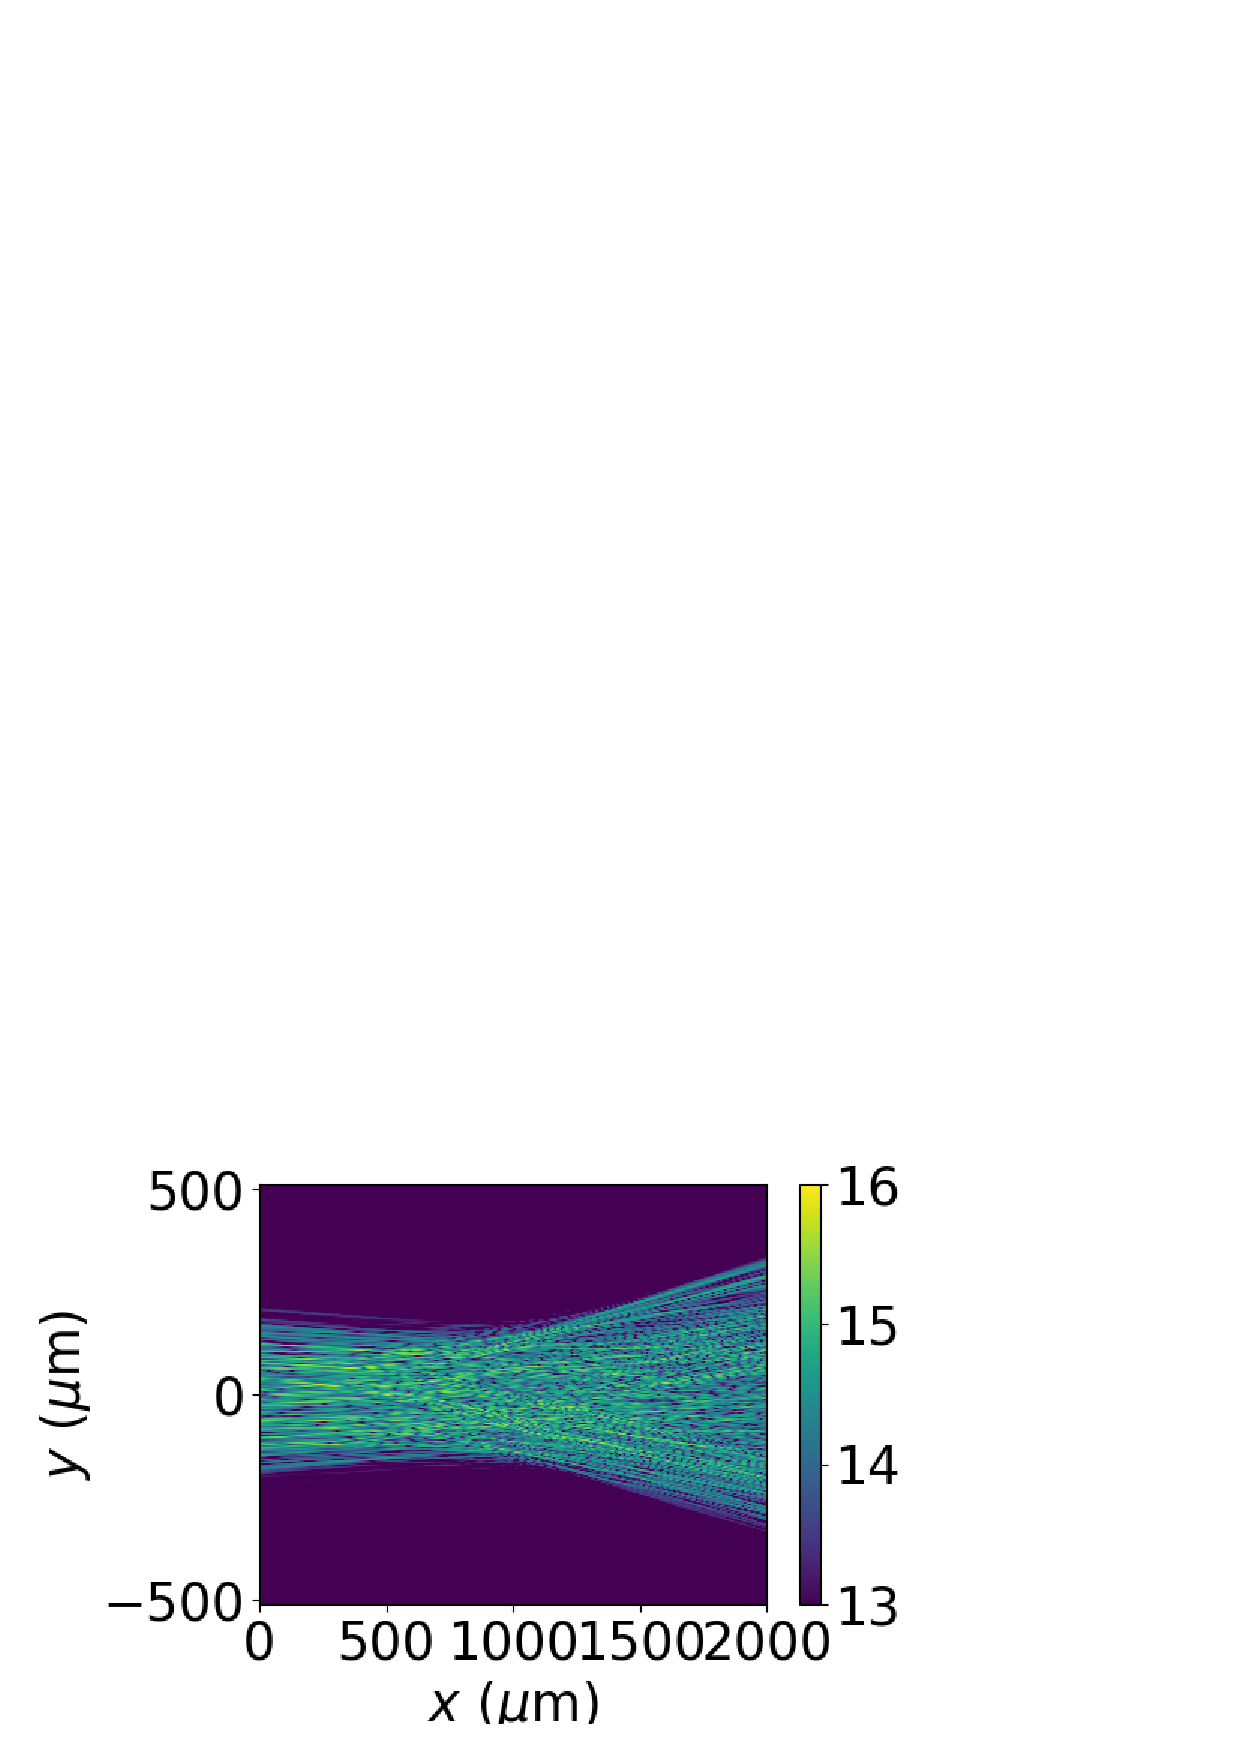
\includegraphics[width=0.3\textwidth]{Fig7a.png}
&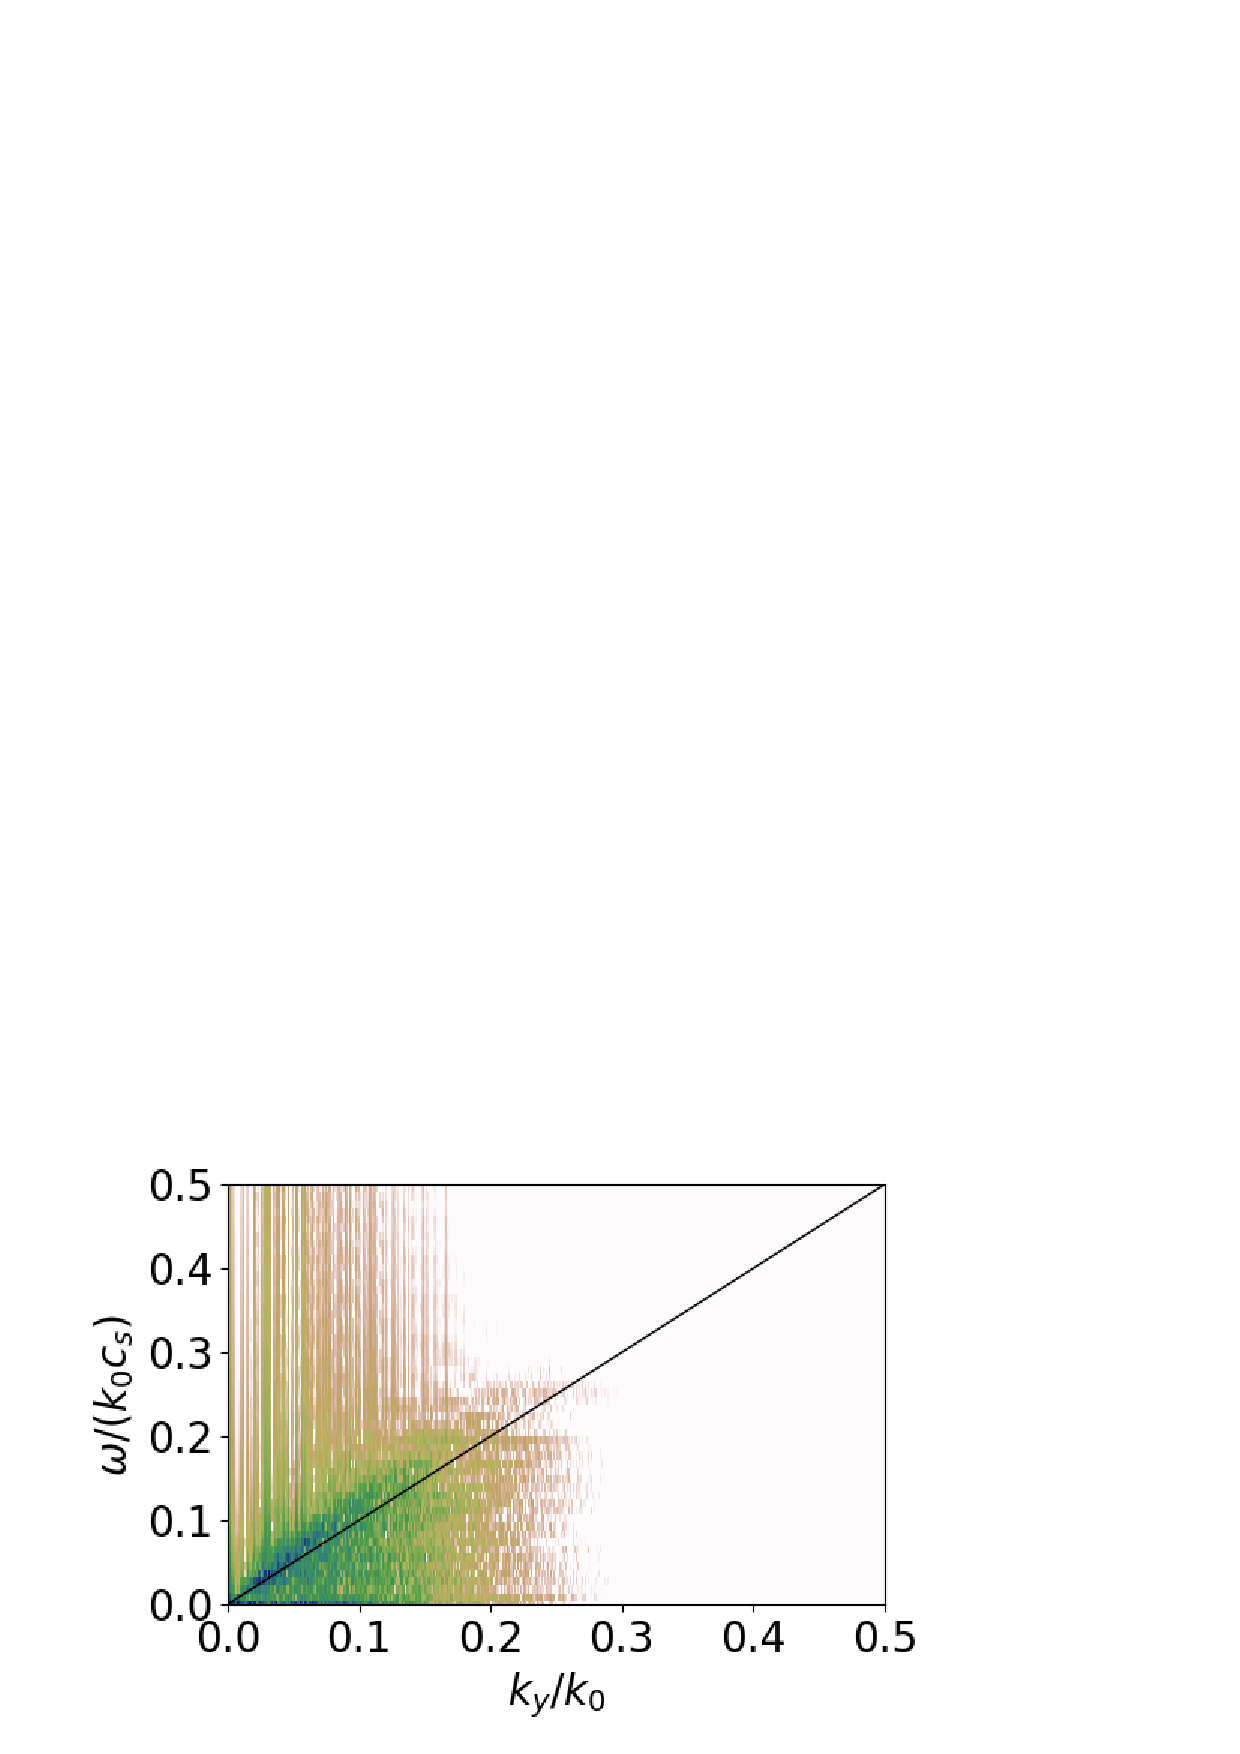
\includegraphics[width=0.3\textwidth]{Fig7b.png}
&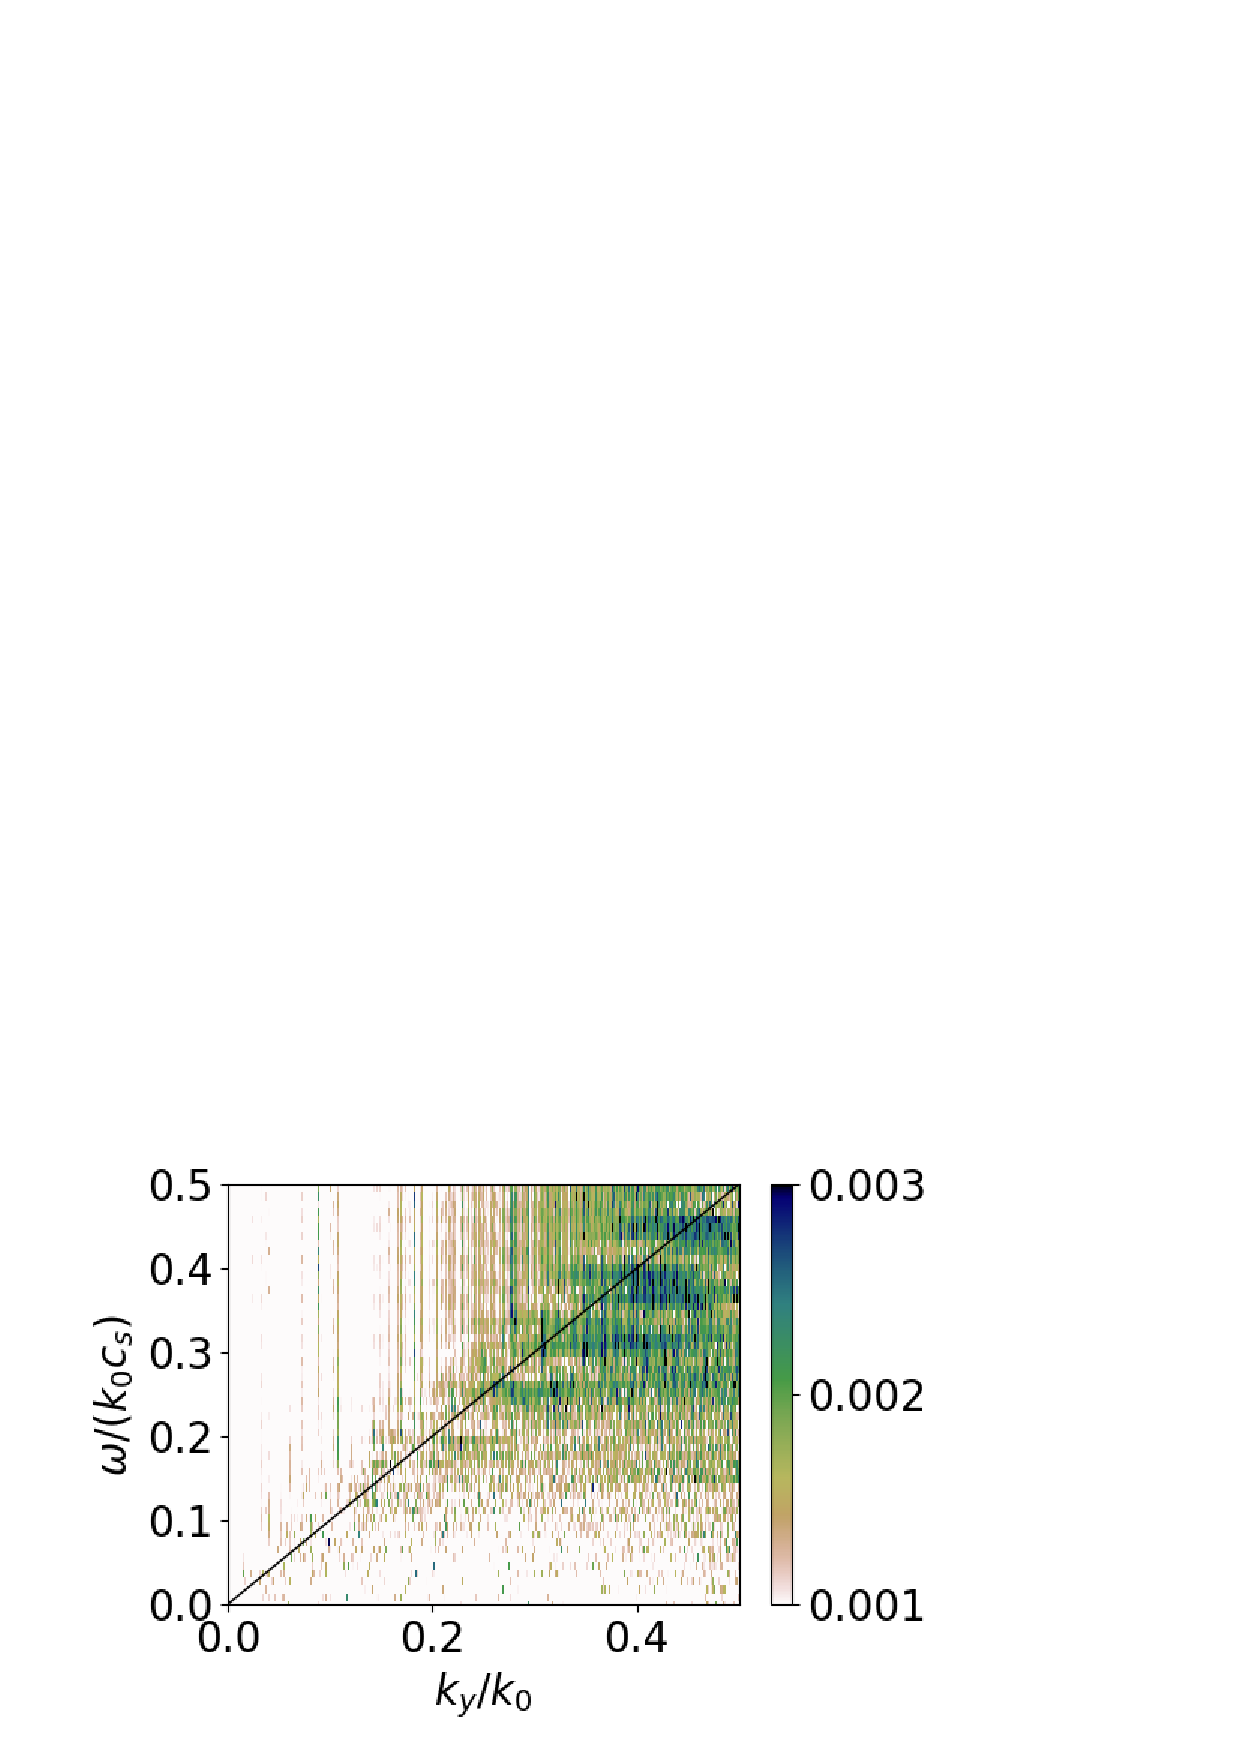
\includegraphics[width=0.3\textwidth]{Fig7c.png}
\end{tabular}
\begin{tabular}{ccc}
(d) $\log_{10}(I \,[\mathrm{W.cm^{-2}}] )$&
(e) Theory, $\log_{10}(\Gamma/k_0)$ &
(f) $\Gamma/k_0$\\ 
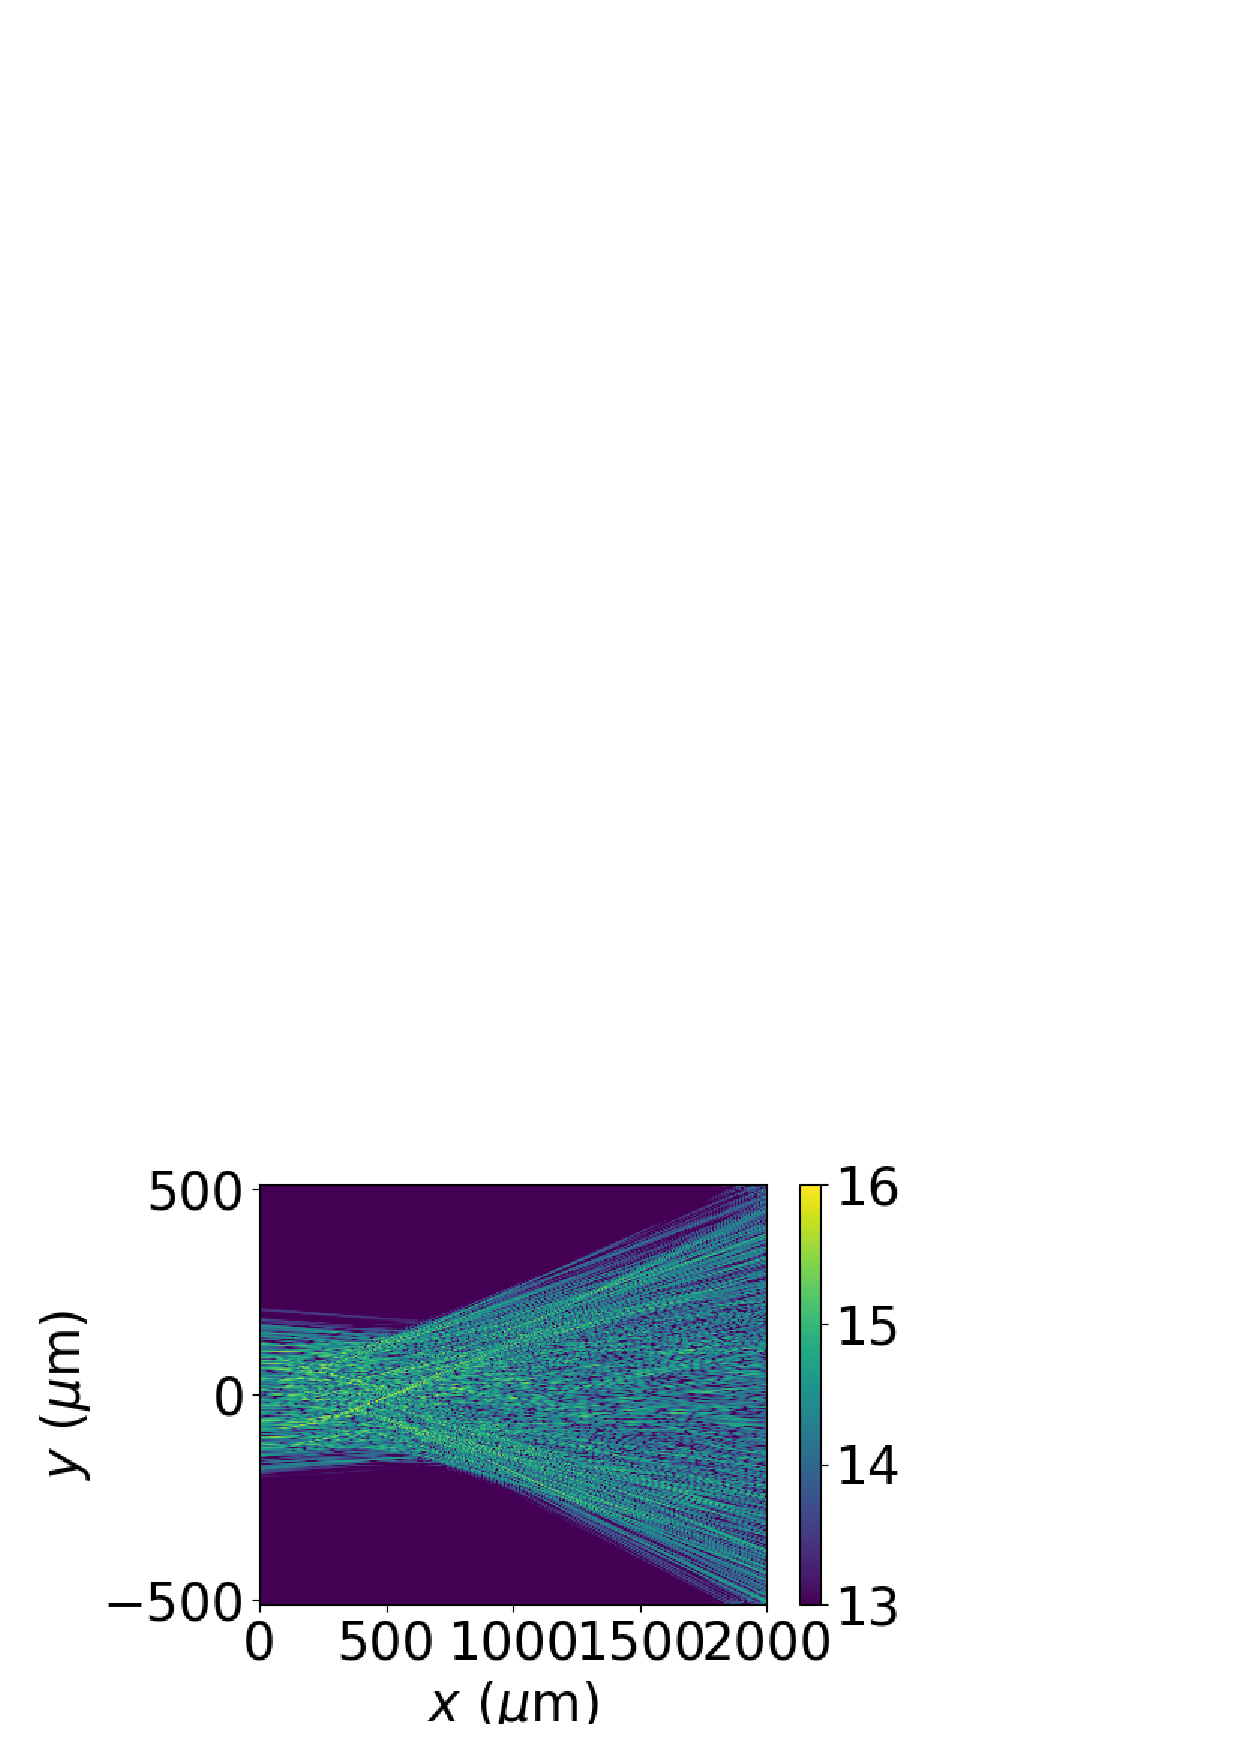
\includegraphics[width=0.3\textwidth]{Fig7d.png}
&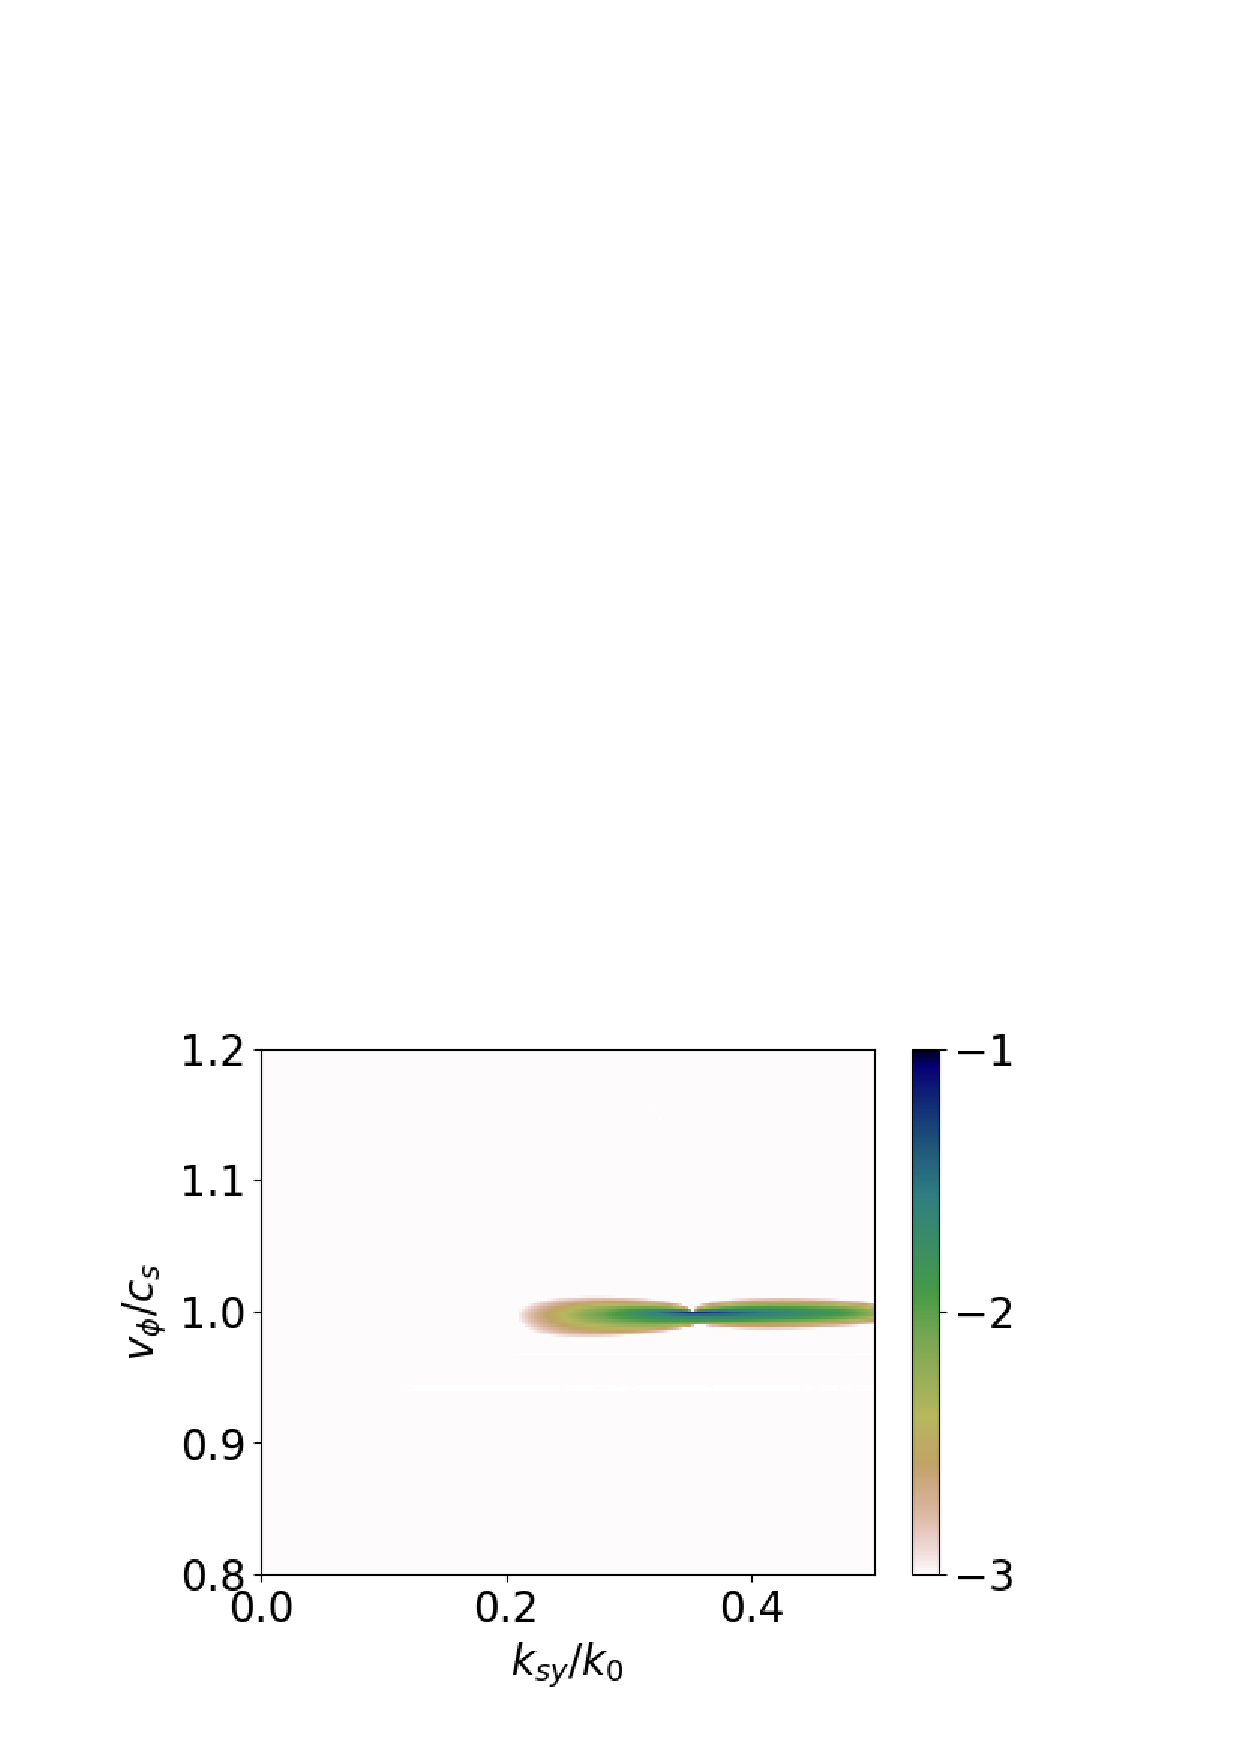
\includegraphics[width=0.3\textwidth]{Fig7e.png}
&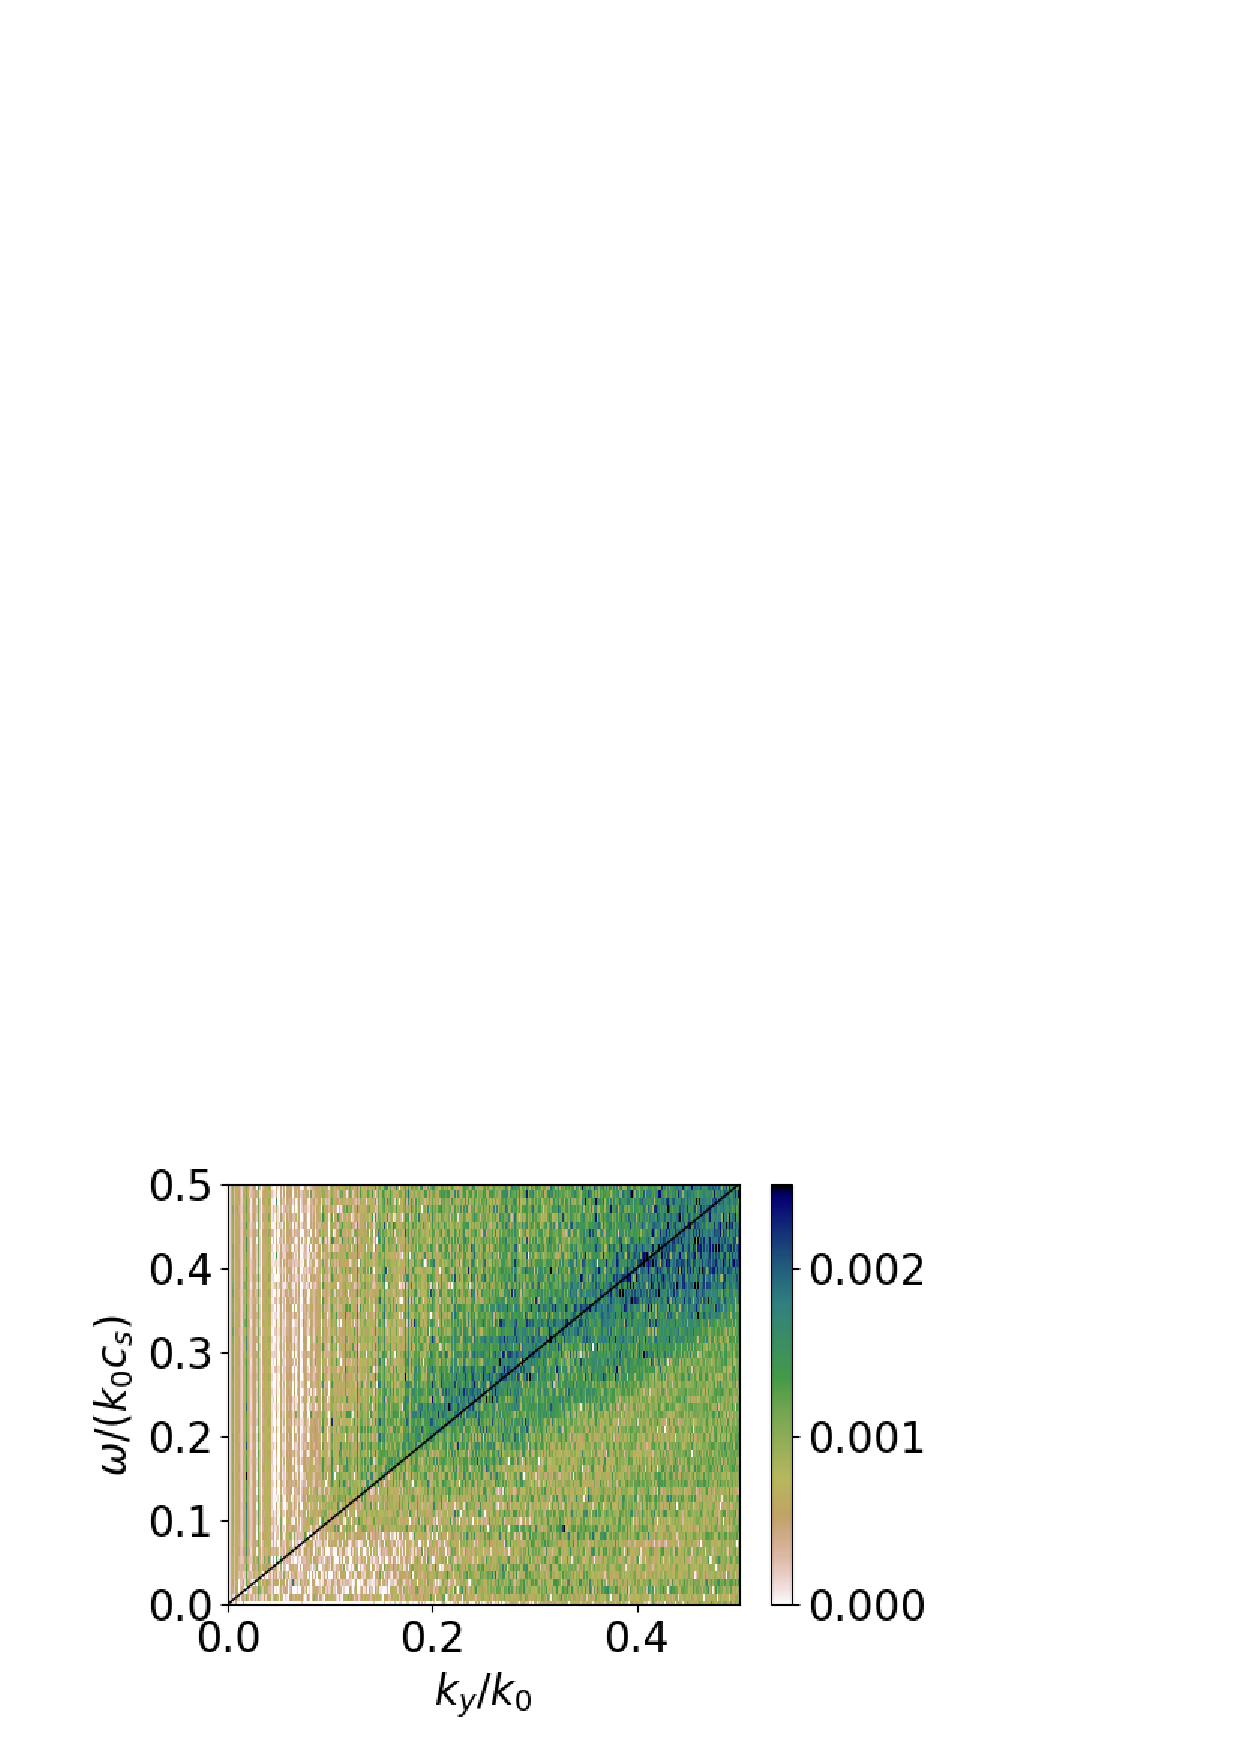
\includegraphics[width=0.3\textwidth]{Fig7f.png}
\end{tabular}
%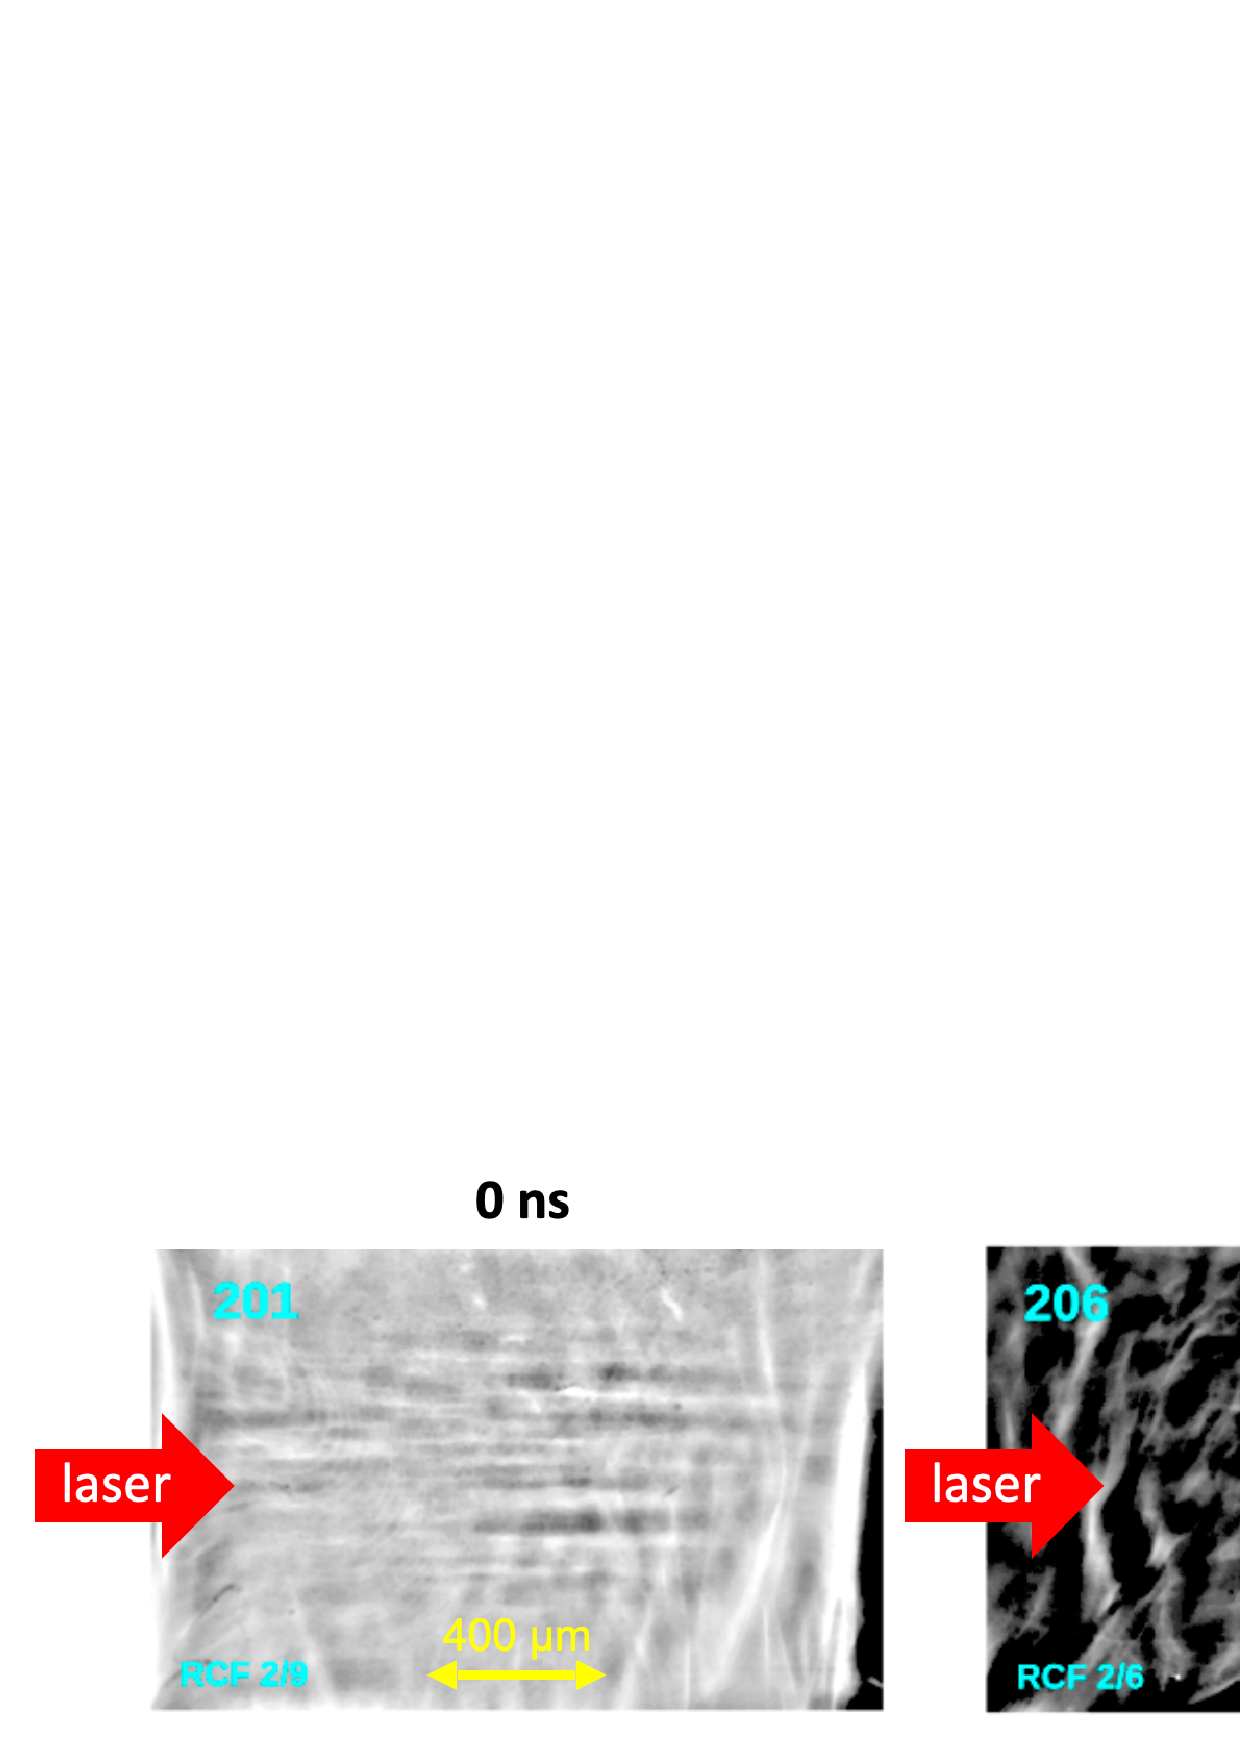
\includegraphics[width=0.5\textwidth]{rcf.png}
\caption{ \label{fig:comphydro}  Simulation results for the H$^+$ plasma with $n_e=0.1n_c$, $T_e=1\,\rm keV$ and $T_i=300\,\rm eV$ (a,b,c) and $T_i=100\,\rm eV$ (d,e,f).
(a,d) Intensity profile at $t=100\,\rm ps$ and (b) spatio-temporal spectrum at $x_2=250\,\rm\mu m$ of $\delta n_e(\omega,k_y,x_2)$. 
(c,f) Effective spatial growth rate extracted from the numerical results between $25$ and $135\,\rm ps$ (c) and between  $40$ and $135\,\rm ps$ (f) following Eq. \eqref{eq:gammah} with $(x_1,x_2)=(200,300)\, \rm \mu m$ (c) and $(x_1,x_2)=(50,150)\, \rm \mu m$ (f).
The corresponding theoretical  growth rates as discussed in Sec. \ref{sec:diperpp} are illustrated in Fig. \ref{fig:disperpp}(c) and panel (e) for $Ti=300$ and  $100\, \rm eV$, respectively.
The acoustic eigenmode $\omega=k_yc_s$ is superimposed on (b,c,f) as black plain lines.
%\textcolor{red}{Pb fig. (d-e).}
}
\end{figure*}
As illustrated in Figs. \ref{fig:comphydro}(a,d),  the RPP beam presents a cone angle increase as soon as $x\gtrsim 500\,\rm\mu m$ at $t=100\,\rm ps$ (and later on). Attributed to the FSBS, its growth may be characterized and compared to our predictions. 

The   density fluctuation spectrum [Fig.  \ref{fig:comphydro}(b) for the case $T_i=300\,\rm eV$] is peaked along the acoustic mode ($\omega=k_yc_s$ as a black solid line) as expected. We may extract an effective spatial growth rate from our numerical results by proceeding to the spatial (in the $y$ direction) and temporal Fourier transform of two lineouts of the density fluctuations, at $x=x_1$ and $x_2$ and following,
\begin{equation}
    \Gamma = \frac{1}{2(x_2-x_1)} \ln \left[\frac{\vert \delta n_e(x_2,k_y,\omega)\vert^2}{\vert \delta n_e(x_1,k_y,\omega)\vert^2}\right] \, , \label{eq:gammah}
\end{equation}
over a time range during which the system does not evolve much. 
For the parameters addressed here, the laser propagation seems to  reach a steady state in a few $10\,\rm ps$, hence the temporal Fourier transform has been performed for $t\in [25,135]\,\rm ps$ and  $[40,150]\,\rm ps$ for  $T_i=300$ and $100\, \rm eV$, respectively. 
Hence, Figs.  \ref{fig:comphydro}(c,f) illustrate for both cases  the effective spatial growth rate  in the plane $(\omega,k_y)$ indicating stability around $\omega=0$, \emph{i.e.} no filamentation instability, consistently with the theoretical predictions and with Figs. \ref{fig:comphydro}(a,d). 
Interestingly, the growth rate along the acoustic mode, marked by the black plain line $\omega=k_yc_s$ in Fig. \ref{fig:comphydro}(c), exhibits a succession of peaks for $k_y>0.2k_0$ consistently with our theory [Fig. \ref{fig:disperpp}(c)]. Their separation of $\sim 0.05 k_0$ correctly agrees with Fig. \ref{fig:disperpp}(c). Moreover, they extend from $k_y \sim  0.2k_0$  to $0.5k_0$, therefore exceeding the initial transverse spectral width of $k_0/2f_\sharp  \simeq 0.062k_0$ and  explaining the large cone angle   observed for $x>500\,\rm\mu m$ in Fig. \ref{fig:comphydro}(a) of $\sim 0.2k_0$ (\emph{i.e.} $11^o$).
When $T_i=100\, \rm eV$, the theoretical predictions [Fig. \ref{fig:comphydro}(e)] yields only one unstable peak located between $\sim 0.2k_0$ and $\sim 0.5k_0$ \tc{with $v_\phi=c_s$}. Likewise, a single large cluster (between  $k_y/k_0\sim 0.2$ and $0.5$) may be recognized  in Fig. \ref{fig:comphydro}(f) \tc{lying on the acoustic trace, $\omega = k_yc_s$ (as black line)} with a dominant feature around $k_y\sim 0.4k_0$, as predicted by our dispersion relations.

%\begin{figure}
%\begin{tabular}{cc}
%(a)     & (b)   \\
%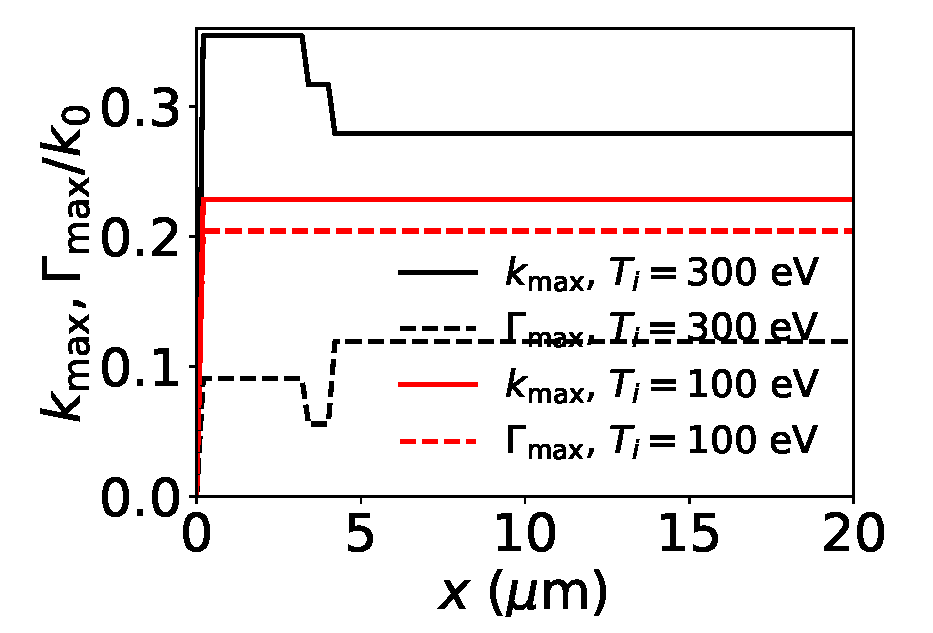
\includegraphics[width=0.245\textwidth]{comp_kmax_gmax.eps}
%&
%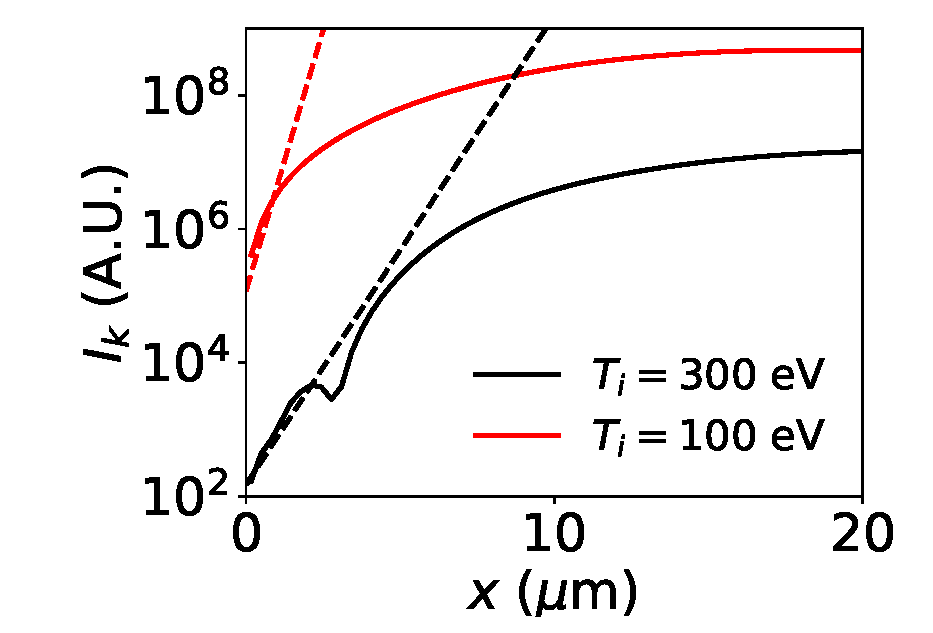
\includegraphics[width=0.245\textwidth]{gmax_eff.eps}
%\end{tabular}
%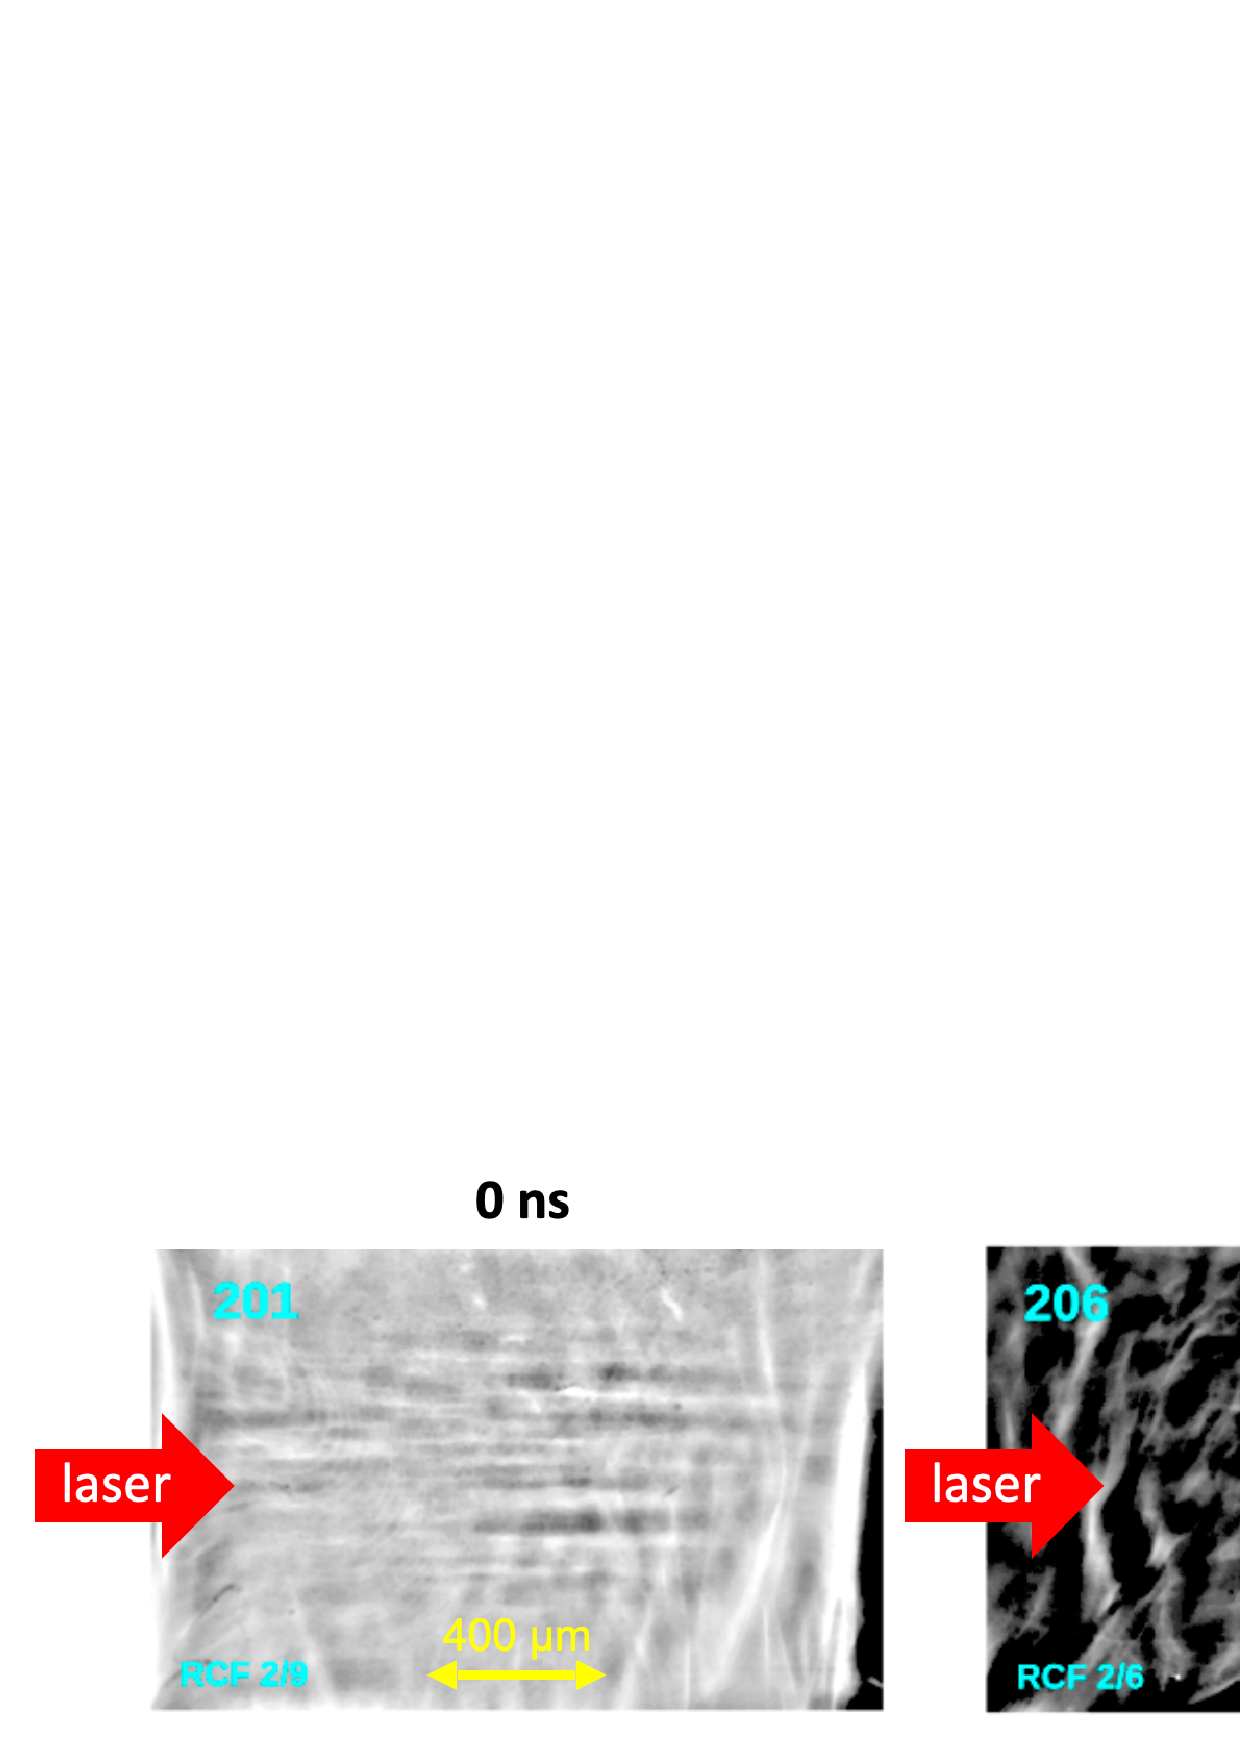
\includegraphics[width=0.5\textwidth]{rcf.png}
%\caption{ \label{fig:geff} 
%(a) Effective growth rate (dashed lines) and wavevector (plaine %lines) which maximises Eq.  \eqref{eq:dI}, %$(\Gamma_\mathrm{max},\mathbf{k}_\mathrm{max})$,  normalized to %$k_0$ for both hydrogen simulations of Fig. \ref{fig:comphydro}.
%(b) Lineout of the intensity transverse Fourier transform at $k_y = 0.26k_0$ ($T_i=300\, \rm eV$, black plain line)  and $k_y = 0.22k_0$ ($T_i=100\, \rm eV$, red plain line). The theoretical exponential growth with $\Gamma_c=0.09k_0$ ($T_i=300\, \rm eV$, black dashed line) and $\Gamma_c=0.2k_0$ ($T_i=100\, \rm eV$, red dashed line) are superimposed. 
%}
%\end{figure}

\begin{figure}

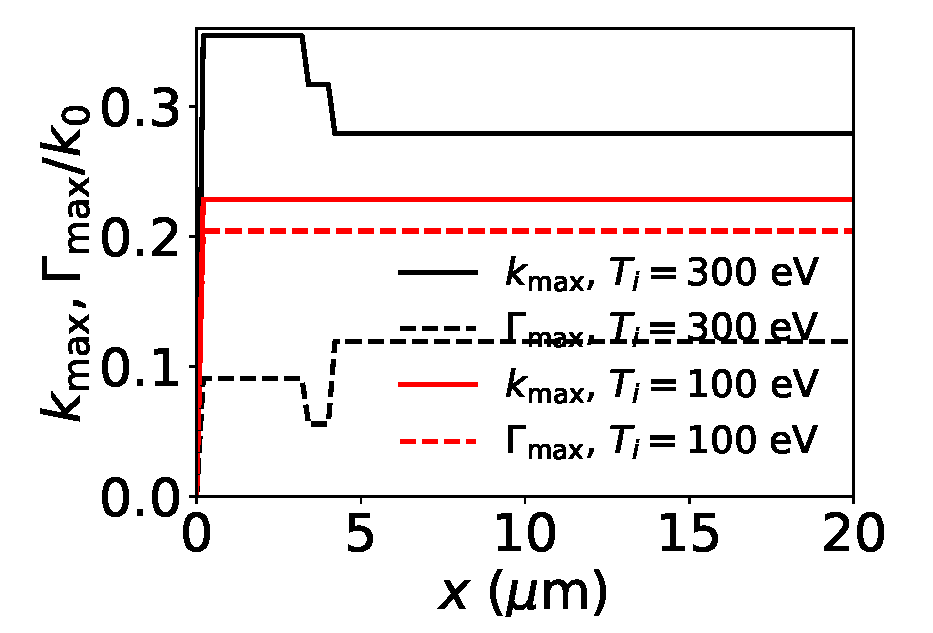
\includegraphics[width=0.99\columnwidth]{comp_kmax_gmax.eps}

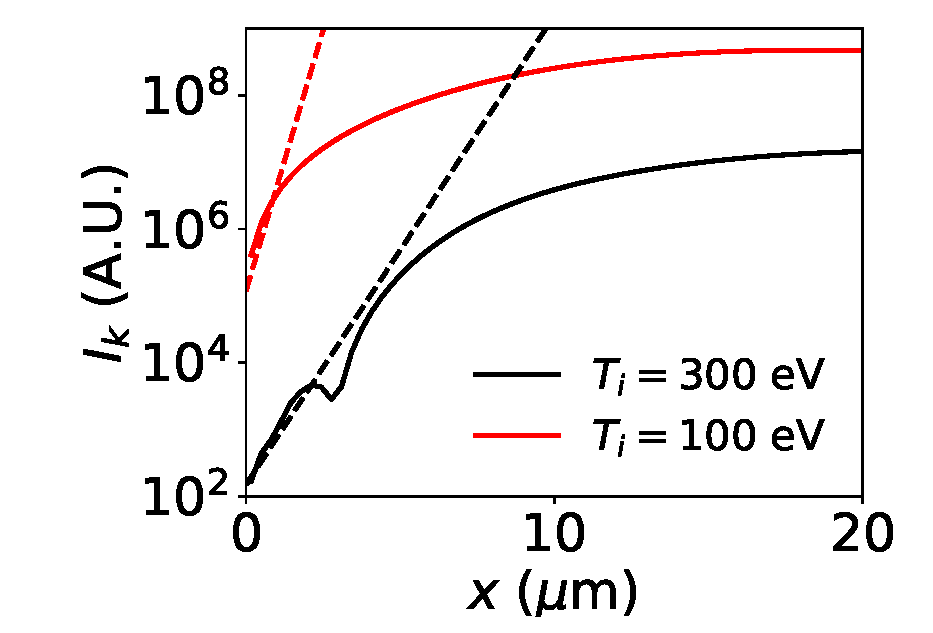
\includegraphics[width=0.99\columnwidth]{gmax_eff.eps}

\caption{ \label{fig:geff} 
(top) Effective growth rate (dashed lines) and wavevector (plain lines) that maximise Eq.  \eqref{eq:dI}, $(\Gamma_\mathrm{max},\mathbf{k}_\mathrm{max})$,  normalized to $k_0$ for both hydrogen simulations of Fig. \ref{fig:comphydro}.
(bottom) Lineout of the intensity transverse Fourier transform at $k_y = 0.26k_0$ ($T_i=300\, \rm eV$, black plain line)  and $k_y = 0.22k_0$ ($T_i=100\, \rm eV$, red plain line). The theoretical exponential growth with $\Gamma_c=0.09k_0$ ($T_i=300\, \rm eV$, black dashed line) and $\Gamma_c=0.2k_0$ ($T_i=100\, \rm eV$, red dashed line) are superimposed. 
}
\end{figure}

Regarding the density fluctuations  growth level, 
%the convective nature of the instability  addressed here complicates the isolation of the spatially growing and propagating  acoustic fluctuations and therefore, the accurate measurement of the exponential slope.
%However, 
the $100-150\,\rm\mu m$-long  and $105-110\,\rm ps$-long window over which the Fourier transform has been performed for resolution purposes, does not allow a quantitative comparison with the theoretical predictions.
%Hence, the validation of the  FSBS spatial growth  of the density perturbation has to settle for a good accordance of the space and time spectrum shape and the assessment of the  multi-unstable acoustic peaks  characterizing the FSBS of a RPP beam.
By contrast, the scattered field  growth is more suitable to quantitative comparisons. Indeed, the linearized paraxial propagation of the perturbed fields $\delta E$, when accounting for diffraction, verifies 
\begin{equation}
    \partial_x \delta E(\mathbf{k}_d,t) + \frac{i\mathbf{k}_d^2}{2k_0}\delta E(\mathbf{k}_d,t) = -\frac{i}{2\pi}\frac{k_0n_0}{2n_c}E_0\otimes \frac{\delta n_e}{n_e} \, . \label{eq:parax}
\end{equation}
For illustration purposes, we will model the spatial growth rate spectrum by a succession of Dirac functions, so that 
\begin{equation}
     \frac{\delta n_e}{n_e}(\mathbf{k}_s) \simeq  \frac{\delta n_0}{n_0} \sum_{\mathbf{k}_c} e^{i\Gamma_{c} x} \delta(\mathbf{k}_s-\mathbf{k}_c)\, , \label{eq:dnparax}
\end{equation}
where $(\mathbf{k}_c,\Gamma_{c})$ are the location and amplitude of the peaks. 
Hence,
the solution of Eq. \eqref{eq:parax}, using the pump fields of Eq. \eqref{eq:erppf},  allows to compute the perturbed fields, $\delta E$, as a function of the phase plate random variables $\Phi_k$. 
\tc{
Using, $\delta E(x=0)=0$, Eqs. \eqref{eq:erppf}, \eqref{eq:parax} and \eqref{eq:dnparax} lead to
\begin{align}
 \delta E(\mathbf{k}_d)=-\frac{i}{2\pi}\frac{k_0n_0}{2n_c} \frac{\delta n_0}{n_0}\frac{E_0}{2N} e^{-\frac{i\mathbf{k}_d^2 x}{2k_0}}   \sum_{\mathbf{k}_c,\mathbf{k}_\perp}\nonumber \\ 
 \left( 
 e^{i\Phi_{\mathbf{k}_\perp}}\delta( \mathbf{k}_d -\mathbf{k}_c-\mathbf{k}_\perp)
 +e^{-i\Phi_{\mathbf{k}_\perp}}\delta( \mathbf{k}_d -\mathbf{k}_c+\mathbf{k}_\perp)
 \right)\nonumber \\ 
 \times \frac{e^{\Gamma_cx+\frac{i\mathbf{k}_d^2 x}{2k_0} }-1}{\Gamma_c+\frac{i\mathbf{k}_d^2 }{2k_0}}  \, .
\end{align}
Finally, the corresponding averaged perturbed intensity [using Eq. \eqref{eq:d}] defined as 
$ \delta I \propto\langle  E_0 \otimes \delta E\rangle $ has  a   piecewise contribution} which  reads
\begin{equation}
\delta I (\mathbf{k}_d)\propto \sum_{\mathbf{k}_c} \frac{e^{\Gamma_c x} -e^{-i( \mathbf{k}_d +\mathbf{k}_c)^2x/8k_0} }{ ( \mathbf{k}_d +\mathbf{k}_c)^2 - 8ik_0\Gamma_c  } \mathrm{H}(2k_m - \vert  \mathbf{k}_d-\mathbf{k}_c \vert) \, , \label{eq:dI}
\end{equation}
where $\mathrm{H}$ is the Heaviside step function.
This demonstrates that although high frequency density fluctuations may grow significantly, the $\sim \mathbf{k}_d^{-2}$ factor in front of the exponential due to diffraction tends to favor FSBS growth for small wavevectors. 
For highly unstable systems such as the one addressed here, saturation occurs rapidly.
Hence, when the pump depletion is reached, the wavevector that saturates first is the one that maximises $\delta I$ and does not necessarily coincide with the fluctuation density growth rate maximum. 
In these conditions, the field effective growth rate and wavevector, (\emph{i.e.}
the effective scattered field f-cone angle), may be related to the wavevector that maximises Eq. \eqref{eq:dI} and the corresponding growth rate peak amplitude and location, $(\Gamma_\mathrm{max},\mathbf{k}_\mathrm{max})$.

Figure \ref{fig:geff}(a) illustrates the spatial evolution of  $(\Gamma_\mathrm{max},\mathbf{k}_\mathrm{max})$ for the two simulations of Fig. \ref{fig:comphydro} and demonstrates that,   the wavevector and peak growth rate that maximize
$\delta I$ remain essentially unchanged over the first 20 microns of the laser propagation (and corresponding to a  $>10^{10}$-factor  increase of  $\delta I$). The exponential growths of $\delta I(k_y=k_\mathrm{max})$ extracted from the hydrodynamic simulations and illustrated in Fig. \ref{fig:geff}(b) as plain lines, correctly agree with our theoretical predictions (as dashed lines) and show that   saturation is reached after $\sim 10\,\rm\mu m$.
Moreover, $k_\mathrm{max}/k_0\simeq 0.28$ and $0.35$ [the location of the growing peaks in Fig. \ref{fig:disperpp}(c) and \ref{fig:comphydro}(e)], corresponding to a beam deflection  of $560$ and $700\,\rm\mu m$ after $2\,\rm mm$ of propagation, compare satisfactorily with Figs. \ref{fig:comphydro}(a) and \ref{fig:comphydro}(d) for $T_i=300$ and $100\, \rm eV$, respectively.
Hence, our dispersion relations are validated quantitatively in the fluid formalism. The kinetic counterpart will be confronted to numerical studies in a future work.

\section{Conclusion}
The spatial growths of the filamentation and of the forward Brillouin instabilities of a RPP beam have been compared in the fluid and kinetic frameworks. Although the latter confirm the importance  of spatial smoothing techniques on the control of the laser filamentation, this instability persists in the case of multi-ion  or cold-enough plasmas.
Albeit hydrodynamic codes predictions are correct regarding the description of the laser filamentation in a single-ion species plasma,
they fail to capture the correct behavior in the multi-ion species case. 
%Provided one accounts for multi-ion species effects and non-local thermal corrections, working in the fluid framework seems to be reasonable regarding the laser filamentation instability.
Moreover, we also conclude that the use of Random phase plates does not guaranty stability of the laser propagation regarding FSBS. RPP beams can suffer large angle scatterings.
Except for a single ion species plasma for moderate to large  $Z_iT_e/T_i$-ratios, the FSBS growth can be imperfectly described in hydrodynamic codes leading to an ill prediction of the beam cone-angle increase and of the plasma smoothing. 
This brings to light the significance of the kinetic damping of driven acoustic waves able to  affect the scattered spectrum.

During the calculation of the spatial growth of the forward instabilities, we neglected the transverse spatial laser envelope and its variations due to diffraction. Hence, our results should remain valid in realistic conditions for large-enough and flat-enough focal spots and for long enough focus. Moreover,  our analytical results are averaged over the random phase plate elements thus failing to capture the corresponding statistical fluctuations. 
\tc{
We also neglected most Coulomb collisions effects on the propagation of acoustic waves, which, in the kinetic multi ion species case might be of importance  \cite[]{POP_Berger_2005b}. 
}

The use of SSD, which  causes the so-called speckles to vanish and change position during the interaction, is known  experimentally to significantly stabilize the pump propagation \cite[]{Berger_1995}. The framework developed in this publication allows to include the spectral dispersion in the dispersion relations of importance for LMJ or NIF like facilities  and is left for future work. Moreover, 
combining our spatial growth rates with our recent Monte-Carlo algorithm~\cite[]{POP_Debayle_2019}  opens the way to the description of the RPP forward Brillouin scattering   in the vastly used ray tracing schemes, possibly greatly improving their predictions regarding high-energy laser experiments. For this end, the impact of a flow on the growth of the FSBS or the filamentation instability must be examined. 
Furthermore, a better  understanding of the competition between the convective or absolute modes in the kinetic framework is required,   as studied  in Refs. \cite[]{phd-Grech,PRL_Grech_2009} for the fluid case  (see Ref. \cite[]{POP_Grismayer_2004}  regarding the stimulated Raman scattering) or  following   Ref. \cite[]{PR_Hall_68}.
Finally, the comparison of our model with NIF or LMJ-relevant experiments is currently underway. 

\section*{Acknowledgements}
We acknowledge important discussions with M. Grech and L. Gremillet. We acknowledge the expert support of the LULI technical teams. We also admit the role of the lockdown following the COVID19 plague for forcing us to take the time to finalize this theoretical work. This work has been done under the auspices of CEA-DAM  and the simulations were performed using HPC resources at TGCC/CCRT and CEA-DAM/TERA.

\section*{Data availability}
The data that support the findings of this study are available from the corresponding authors upon reasonable request.

\appendix
\section*{Appendix: constraining $Z_iT_e/T_i$ in the experiment of Sec. \ref{sec:xp}}
\label{sec:ztesti}
%\setcounter{equation}{0} 
%\renewcommand{\theequation}{A\arabic{equation}}
%\setcounter{figure}{0} 
%\renewcommand{\thefigure}{A\arabic{figure}}
\begin{figure}
\begin{tabular}{cc}
(a) FFT of transverse lineout&
(b) Peak evolution\\
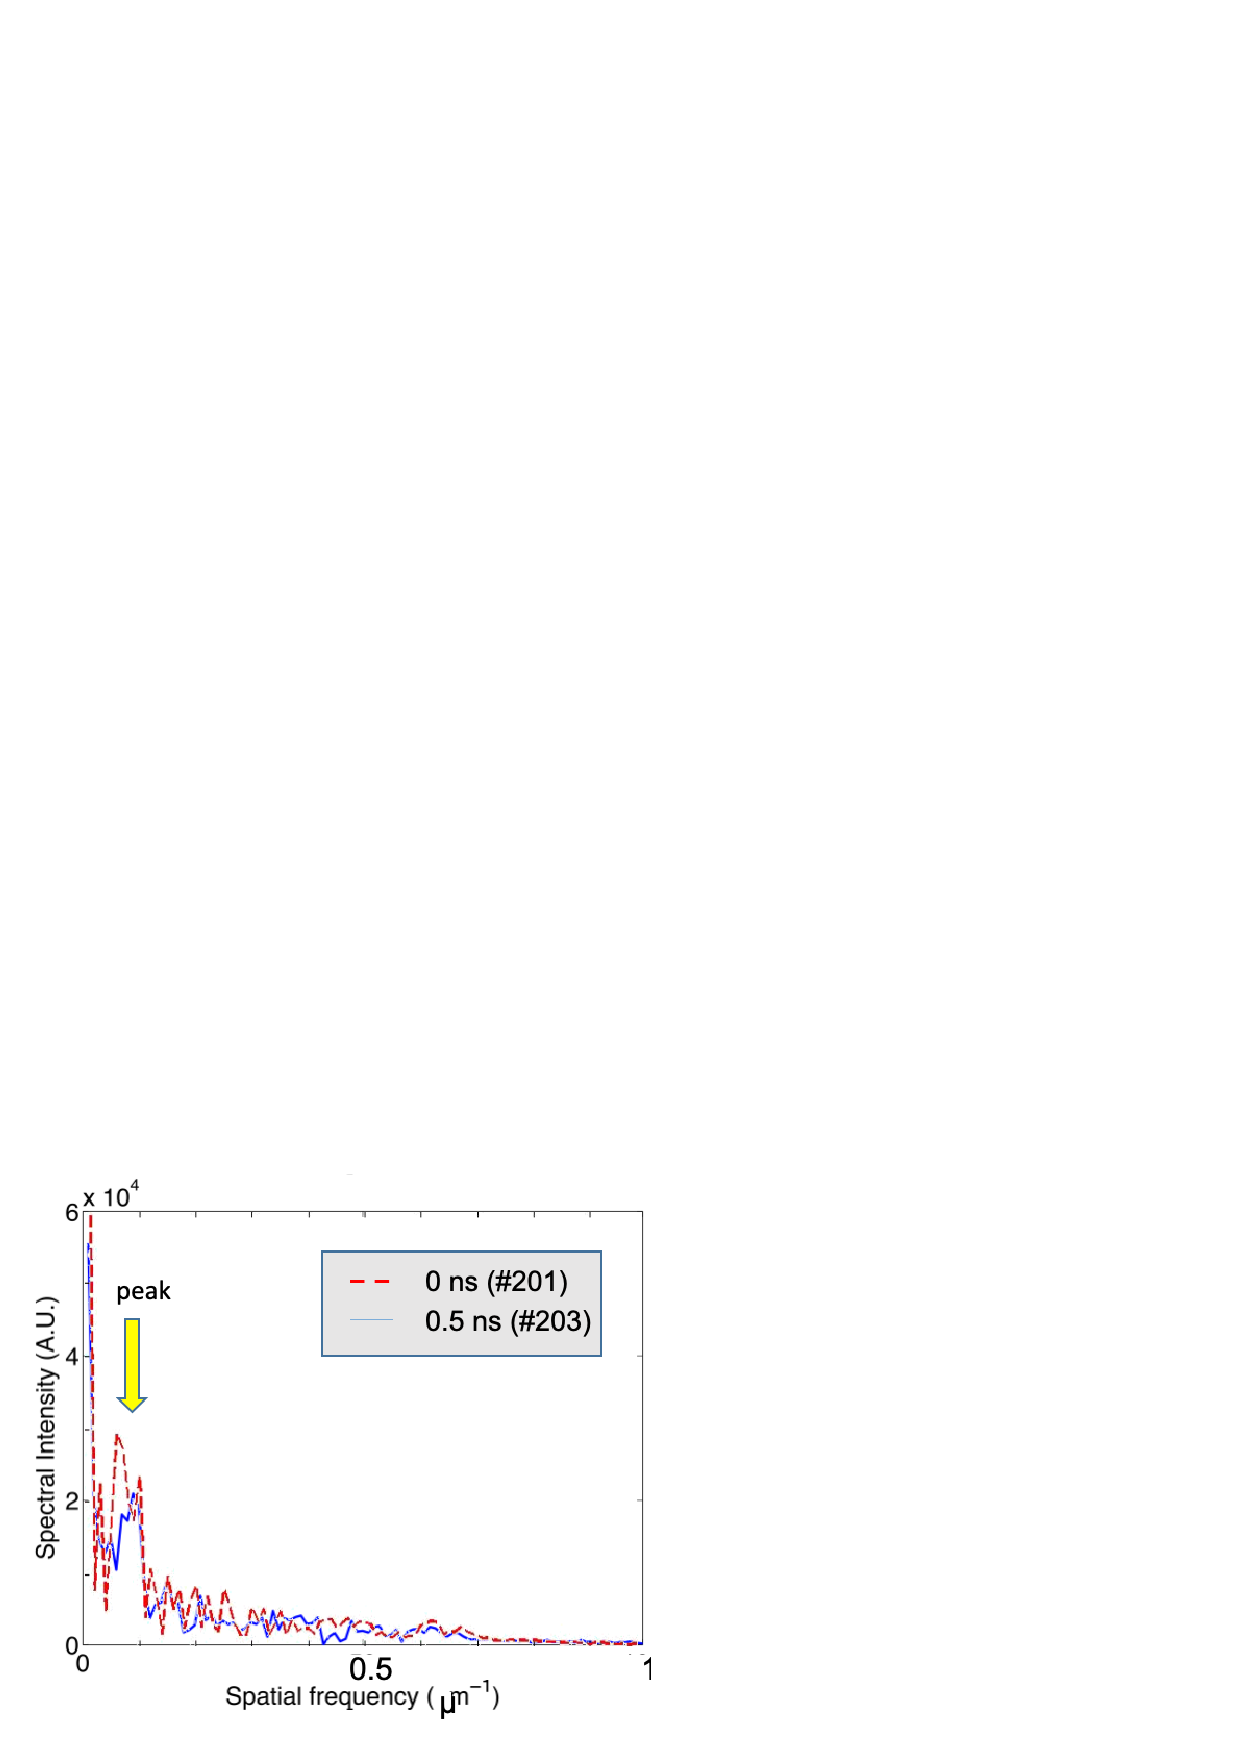
\includegraphics[width=0.24\textwidth]{fucshsfft.png}& 
\includegraphics[width=0.22\textwidth]{fuchsztesti_new.eps}
\end{tabular}
\caption{ \label{fig:xpfuchs_ap}  
(a) Fourier transform of a central lineout across RCF similar as those shown in Fig. \ref{fig:xpfuchs_xp}(b), unravelling a peak at the dominant wavelength. The two curves correspond to two different shots, taken at different times, as indicated in inset.
(b) Temporal evolution of the peak amplitude (blue circles) observed in the Fourier transform identified by the yellow arrow in panel (a). Each point correspond to a different shot, where the time of the proton probing was changed with respect to the interaction laser propagating in the plasma [see examples of probing at two different times in  Fig. \ref{fig:xpfuchs_xp}(b)]. A decreasing exponential slope,  $\exp(-\nu t)$, is plotted for a Landau damping frequency given by $\nu=\gamma_0c_s2\pi/[77\,\rm\mu m]$ with the use of  Eq. \eqref{eq:g0} for a He$^{2+}$ plasma with \tc{$T_e=310\,\rm eV$} [see Fig. \ref{fig:xpfuchs_th}(a)] and various $Z_iT_e/T_i$.
}
\end{figure}
Figure \ref{fig:xpfuchs_ap}(a) shows the Fourier transform of a RCF transverse lineout pointing out to a peak around a spatial frequency of  $2\pi/\lambda_s\sim 0.08\, \rm \mu m^{-1}$, \emph{i.e.} a wavelength of $\lambda_s \simeq 77\, \rm \mu m$.
Moreover, the comparison of the peak position at different times (blue plain line at $t=0\,\rm ns$ and red dashed line $t=0.5\,\rm ns$) demonstrates that the dominant wavelength remains mostly unchanged.  In that condition, and noting that the probing proton deflection results from an electric field, the RCF dose modulation level depends mainly on the electron pressure fluctuations amplitude \cite[]{RSI_protograhyb}.
Hence, the peak temporal evolution of the experimental signal [blue circles in Fig. \ref{fig:xpfuchs_ap}(b)] correlates with the damping of the lingering acoustic waves, previously triggered by the filamentation instability over the first nanosecond of  the interaction beam.
In this low density configuration ($n_e/n_c\simeq10^{-2}$), 
we may therefore directly compare this decrease with an exponential slope, $\delta n_e \propto \exp(-\nu t)$ where $\nu = \gamma_0 c_s 2\pi/\lambda_s$ is the Landau damping acoustic rate. The calculations for a He$^{2+}$ plasma with \tc{$T_e=310\, \rm eV$} [as suggested by  Fig. \ref{fig:xpfuchs_th}(a)] and  for three different values of $Z_iT_e/T_i$ illustrated in  Fig. \ref{fig:xpfuchs_ap}(b) demonstrate that $Z_iT_e/T_i=5$ reproduces correctly the experimental data. The experimental point at $t=0.5\,\rm ns$ is more consitent with the red curve which may suggest a value of  $Z_iT_e/T_i $ larger than $5$ earlier. Because of the available experimental data and the weak dependence of the filamentation growth rate on $Z_iT_e/T_i$, choice has been made to set the ratio to  $5$ for the analysis of Sec. \ref{sec:xp}.

\bibliography{biblio}
\end{document}
